\documentclass[a4j,a4paper,11pt,oneside,openany,uplatex]{jsbook}
\usepackage{dcolumn,multirow,ccaption}

%図表の個数などの設定。
\setcounter{topnumber}{4}
\setcounter{bottomnumber}{4}
\setcounter{totalnumber}{4}
\setcounter{dbltopnumber}{3}

\renewcommand{\topfraction}{.95}
\renewcommand{\bottomfraction}{.90}
\renewcommand{\textfraction}{.05}
\renewcommand{\floatpagefraction}{.95}

%使用するパッケージを記述。
\usepackage{amsmath, amssymb} %複雑な数式などを打つときに使用。
\usepackage{bm} %数式環境内で太字を使うときに便利。
\usepackage{graphicx} %画像を挿入したり、テキストや図の拡大縮小・回転を行う。
\usepackage{subfigure} %図を並べる(今はsubfigとかsubcaptionとかが推奨らしい。よく知らない)
\usepackage{verbatim} %入力どおりの出力を行う。
\usepackage{ascmac} %テキストを枠で囲んだりできるが、微小なズレがでたりする。
\usepackage{makeidx} %索引を作成できる。
\usepackage{dcolumn} %表の数値を小数点で桁を揃える。
\usepackage{lscape} %図表を90度横に倒して配置する。
\usepackage{setspace} %行間調整。
\usepackage{multirow}
\usepackage{float} %図を入れるときに何々する
\usepackage{grffile} %デフォルトでmultidotがtrue
\usepackage{siunitx} %SI単位(国際単位系)を出力する


%余白の設定。
%\usepackage[top=30truemm,bottom=30truemm,left=25truemm,right=25truemm]{geometry}

% 高さの設定
% \setlength{\textheight}{\paperheight}   % ひとまず紙面を本文領域に
% \setlength{\topmargin}{3.6truemm}      % 上の余白を29mm(=1inch-5.4mm)に
% \addtolength{\topmargin}{-\headheight}  % 
% \addtolength{\topmargin}{-\headsep}     % ヘッダの分だけ本文領域を移動させる
% \addtolength{\textheight}{-50truemm}    % 下の余白も25mmに
% %% 幅の設定
% \setlength{\textwidth}{\paperwidth}     % ひとまず紙面を本文領域に
% \setlength{\oddsidemargin}{-5.4truemm}  % 左の余白を20mm(=1inch-5.4mm)に
% \setlength{\evensidemargin}{-5.4truemm} % 
% \addtolength{\textwidth}{-40truemm}     % 右の余白も20mmに

\usepackage{tablefootnote} % use footnote in table

%ハイパーリンクの設定
\usepackage[dvipdfmx]{hyperref}
\usepackage{pxjahyper}
\hypersetup{% hyperrefオプションリスト
 colorlinks=true,
 }
%参考文献の設定 
\usepackage{natbib, aas_macros}
\citestyle{aa}

\renewcommand{\labelenumi}{(\arabic{enumi}) } %enumerate環境を1. 2.の形式から(1) (2)の形式へ変更(文書全体)。
\renewcommand{\appendixname}{付録 }

\usepackage{mathrsfs}

%listing ソースコードを綺麗に表示させるためのパッケージ
\usepackage{listings}
\usepackage{color,colortbl}
 
\definecolor{codegreen}{rgb}{0,0.6,0}
\definecolor{codegray}{rgb}{0.5,0.5,0.5}
\definecolor{codepurple}{rgb}{0.58,0,0.82}
\definecolor{backcolour}{rgb}{0.95,0.95,0.92}
 
\lstdefinestyle{mystyle}{
    backgroundcolor=\color{backcolour},   
    commentstyle=\color{codegreen},
    keywordstyle=\color{magenta},
    numberstyle=\tiny\color{codegray},
    stringstyle=\color{codepurple},
    basicstyle=\footnotesize,
    breakatwhitespace=false,         
    breaklines=true,                 
    captionpos=b,                    
    keepspaces=true,                 
    numbers=left,                    
    numbersep=5pt,
    showspaces=false,                
    showstringspaces=false,
    showtabs=false,                  
    tabsize=2
}

% 余白の調整
\usepackage{geometry}
\geometry{left=25truemm,right=25truemm,top=30truemm,bottom=25truemm}
 
\lstset{style=mystyle}

%\setcounter{tocdepth}{2} %項レベルまで目次に反映させるコマンド。

\begin{document}
%%
%% ccaption.sty用
%%
 \setlength{\abovecaptionskip}{0pt}
 \setlength{\belowcaptionskip}{0pt}
 \captiondelim{: }

%%
%% dcolumn.sty
%%
\newcolumntype{.}{D{.}{.}{-1}}

\renewcommand\arraystretch{1.1}

\begin{titlepage}
\begin{spacing}{2.3}

\begin{center}
\vspace*{80truept}
{\huge 東京大学大学院}\\
{\huge 理学系研究科天文学専攻}\\
\vspace{20truept}
{\huge 2018年度 \ 修士論文}\\
\vspace{50truept}
{\huge 太陽運動の解析における星の速度分散の効果の定量評価}\\
%{\LARGE ------サブタイトル------}\\ % サブタイトル(なければコメントアウト)
\vspace{100truept}
{\LARGE 柏田 祐樹}\\ % 著者
{\LARGE 学生証番号:35-176115}\\ % 学籍番号
{\LARGE 指導教員:郷田直輝}\\ %指導教員
{\LARGE 2019年1月28日}\\ % 提出日
\end{center}

\end{spacing}
\end{titlepage} %「表紙.tex」というファイルを同じディレクトリ上においておくこと。
%
\frontmatter

\tableofcontents

 % 本文
 %本文は章や節ごとに分割して別々のファイルにして管理し、\input{}で挿入していくのがよいだろう。
\mainmatter

\chapter*{研究概要}
本論文では、観測データの解析で正しい値を得るために模擬データの解析を行うことで太陽系と太陽近傍星の運動を調べ、その結果を踏まえて観測データ解析も行いオールト定数と太陽運動を測定した。Oort-Lindbladモデルを用いることでオールト定数と太陽運動を得ることができるが、モデルでは速度分散が非常に小さい速度場を仮定している一方実際の銀河円盤星は無視できない程度の速度分散を持っていることが近年明らかになっている。また、解析の際には十分な星の数が必要だったり、モデルでは6次元位相空間 (位置の3次元と速度の3次元) データを用いるものの、観測データの不足から、そのうちの1次元 (視線速度) が含まれていない解析がなされていたりと、先行研究の解析にはまだ問題点がある。さらに、太陽運動の銀河回転方向成分$V_{\odot}$はまだ不定性が大きいことも問題である。

そこで、模擬データの生成・解析から速度分散の大きさ、視線速度の有無、サンプル数などの解析結果への効果を調べたところ、特に速度分散によるasymmetric driftの影響が大きく、古い星の解析で$V_{\odot}$を非常に大きく値を間違えて測定することが判明した。その他の影響として、サンプル数と視線速度の有無が解析の精度に対して大きく影響することが分かった。

観測データ解析では、Gaia Data Release 2から約100,000個の星の位置天文データから、局所静止基準に対する太陽系の運動とオールト定数の決定を行った。先行研究の太陽系運動とオールト定数の測定では、解析に視線速度を用いていなかったり、星の選び方にムラがあったりと先行研究で推定された星の年齢の値を用いることで、年齢ごとのサンプルで解析を行った結果、どのパラメータも年齢依存性を持つことがわかった。特に太陽運動の銀河回転方向成分$V_{\odot}$はサンプルの年齢と強い正の相関があり、これはにasymmetric driftの効果によるものであると考えられ、この傾向は模擬データで予想された結果と一致した。また、asymmetric driftでは天の川銀河のスケール長に依存することから、使用するスケール長の値によって得られる$V_{\odot}$の値は異なるものが得られた。さらに、年齢依存性はあるものの、先行研究と比べて妥当な値が得られた。最後に、本論文ではスケール長を年齢の関数で表して解析することで$V_{\odot}$の年齢依存性を解消することを目指した。
\chapter{イントロダクション}
\section{太陽運動・銀河回転パラメータ決定の現状・課題}
% * 1.1 歴史的流れ ← 適切なタイトルに変える
% せっかく書いてくれましたが、ちょっとMilky Wayの発見までの
% 歴史的流れが長いかなぁ、という印象です。
% それに対して、今回の修論の主題に関わる内容の
% 歴史的な流れ (LindbladやOortのこと) の分量が少ないですね。。
% Oortの後に、チャンドラセカールによる一般化が続くと思います。

% 天の川銀河が円盤状の形をして回転していることがわかったのは、最近200年のことである。18世紀にウィリアム・ハーシェル (William Herschel) は600以上の異なる場所で空を観測し、全ての星が同じ輝度を持ち、地球からの各星までの距離を見積もることができると仮定した。彼はこのデータを使って数えた星と地球からの距離を組み込んだ空全体の地図を作成した (図\ref{Herschel})。
% \begin{figure*}[htbp]
% \begin{center}
% 	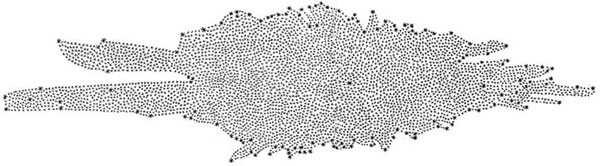
\includegraphics[width=8cm]{fig/Herschel.jpg}
% 	\caption{天の川のさまざまな部分の星の数を数えたことから導かれた天の川の地図 (\cite{Herschel1785})。中心付近に位置する黒い点が太陽を表している。}
% 	\label{Herschel}
% \end{center}
% \end{figure*}
% 彼はこの研究から、太陽は天の川の中心あるいは中心付近に位置しているという結論を出した。また、ハーシェルの示した恒星の分布は、直径約2 kpc、厚さ約400 pcほどのものであった。その後、20世紀初頭にカプタイン (Jacobus Kapteyn) は世界中の天文学者の助けを借りてハーシェルの天の川の地図よりも高精度な地図を作成した。カプタインが示した天の川は、直径約17 kpc、厚さ約3 kpcというものであった。しかし、カプタインもまた太陽は天の川の中心に位置していると考えていた。その理由は、実際には銀河中心に星が密集しているが、星間塵による星の光の強い星間吸収の影響でよく見えず、その結果どの方向でも星は同じように分布しているように見えるためである。

% 1920年、シャプレー (Harlow Shapley) によって、銀河系中心という特別な場所に太陽が位置するという理論を覆された。彼は最も近い球状星団に含まれること座RR型変光星を観測し、年周視差と変光星の周期-光度関係を利用することでその星団までの距離を測定した。同様に変光星を利用していくつかの球状星団の天球面上の位置と距離を決定していくと、銀河系の全体像が浮かび上がった。すると、彼は球状星団が射手座の方向のある一点の周囲に球状に分布していることを発見した。その後、その点を銀河系の中心として提案し、太陽は銀河系の中心から離れた場所に位置していることを示した。この発見は地動説に次ぐ天文学上の最も重要な発見である。

%太陽系は現時点では生命が存在することが確認されている唯一の惑星系である。太陽系は約46億年の歴史の中で、誕生から22回ほど銀河中心の周りを回転してきたと考えられる (\cite{Adams2010})。太陽系の起源と誕生からの歴史を決定することは、太陽系に生命が誕生し、生存を続けている理由を明らかにする方法の1つとなる。力学的なアプローチとしては、太陽系を含めた恒星系の回転運動を決めることが必要不可欠となる。太陽運動とオールト定数を決定することは太陽系が描いてきた軌道を知るための重要な方法の1つである。太陽系の軌道を決定できれば、太陽系がどのような環境で生まれ、どのような歴史を辿ってきたのかが分かれば、太陽系のような惑星系の形成に制限をつけられる可能性がある。

天の川銀河円盤は自己重力による重力ポテンシャルから受ける中心力と回転による遠心力とがつり合って回転を続けられている。つまり、銀河系の各半径での天体の回転運動は質量分布を反映したものとなる。したがって、銀河系円盤の回転運動の様子を理解することは、天の川銀河の動力学を理解する上で非常に重要である。さらに、銀河系内での太陽系の運動を調べることは、太陽系がどこで生まれたかを知るヒントとなる上、銀河系内の力学構造を解釈するためには天体が銀河系中心に対してどのような速度で動いているのかを知る必要があるため、観測した天体の運動速度に対して太陽系の運動速度で補正する形で用いる必要があることから、位置天文学や銀河動力学において主要な課題の1つとなっている。

天の川銀河が回転していることが定着したのは天文学の長い歴史の中でもこの100年のことである。1926年、リンドブラッド  (Bertil Lindblad) はカプタイン (Jacobus Kapteyn) によって20世紀初頭に研究された恒星の運動の様子は銀河系回転によるものあると説明した。彼は、銀河中心に近い星は銀河中心から離れた星よりも速く回転することを提案した。その後オールト (Jan Oort) は、多くの星の速度を観察して1927年にリンドブラッドの理論を証明し、さらにその理論を修正した。彼はオールト定数$A,B$を導入し、銀河系が差動回転していることを示した。また、オールトは太陽系が銀河中心から約10 kpcの距離に位置していると計算した。これらの研究により、太陽系は天の川銀河の円盤の中を他の星と共に回転している描像が明らかとなった。

太陽近傍の星の運動は系統 (平均) 運動にランダム運動 (特異運動) を足したものとして解釈される。円盤銀河では、系統運動が特異運動に比べて支配的である。そのような恒星系は力学的に冷たいと言われる。すなわち、特異運動が系統運動に対して無視できるような系である。例えば、太陽近傍では円盤面の速度分散すなわち特異運動の大きさは古い星の恒星円盤では\SI{45}{km.s^{-1}}、誕生初期の星では\SI{18}{km.s^{-1}}である一方、系統運動は\SI{200}{km.s^{-1}}のオーダーである。特異運動が消える力学的に冷たい極限では、系統運動は重力ポテンシャルによって生まれる閉じた軌道に沿ったものになる。したがって、銀河系回転は重力ポテンシャルから受ける中心力と遠心力とのつり合い、すなわち回転平衡によ
って支えられていることから、天の川銀河のポテンシャルと質量分布は恒星系の系統運動から得ることができる。

\cite{Oort1927a}は、銀河系円盤を回転している天体が閉じた軌道を描いている、すなわち銀河系円盤は力学的に冷たい系であると仮定し、太陽近傍星の位置・速度の観測量を銀河系回転パラメータ$A,B$で記述するモデルを考えた。この$A、B$はいわゆるオールト定数であり、それぞれ銀河回転方向の剪断成分、回転成分を表す。\cite{Chandra42}は、オールトのこのモデルを銀河系円盤の持つ非対称な系統運動の速度場にも適用できるように拡張し、新たな定数$C,K$を導入した。$C、K$はそれぞれ動径方向の剪断成分、発散成分を表す。本論文では、彼らによって構築されたモデルをOort-Lindbladモデル、またこのモデルによる解析をオールト解析と呼ぶことにする (\cite{Oort1927a},\cite{Lindblad1927},\cite{Chandra42})。

% 研究のIntroduction (研究背景・基本事項)、定性的に書く (定量的な事は2章で)
% あと最後に、先行研究 (Olling & Dehnen 2002; Bovy 2017; Vickers & Smith 2018など) で
% 何がどこまでわかっていて、何がわかっていないのかを書いて、
% それを踏まえて、今回の修論の研究のポイントとの違いをしっかり書かないとダメです。
% これが「研究動機」になるはずです。

% * 1.2 現状・課題 ← 適切なタイトルに変える
% 前のセクションでは銀河回転 (オールト定数) の話だったので、
% それに関する「現状・課題」を書いてあるのかと思ったら、
% 急に「太陽運動」の話になっていて、これでは「現状・課題」ではないと思います。
% また「現状」については、書いてあるように見えますが 
% (本当はもっと最近の研究まで書いたほうがよいですが)、
% 「課題」が明確に書かれていない印象です。

これまで、いくつかの先行研究によって太陽運動 (太陽の特異運動) と銀河系速度場パラメータ (オールト定数) が求められてきた。太陽系近傍の銀河系回転運動の測定には星や星間ガスの位置と速度の情報が用いられるが、簡単ではない。星は速度分散が大きい一方、星間ガスは距離測定が難しいという問題がある。本論文では星に対してオールト解析を行うが、先述の通りOort-Lindbladモデルは力学的に非常に冷たい系、すなわち速度分散が回転運動に比べて非常に小さく無視できるような系を仮定したモデルである。しかし、実際に天の川銀河円盤は無視できない程度の速度分散を持っており、解析においては速度分散を考慮しなくてはならない。また、セファイドやOB型星など非常に若い、かつ重い星は質量が重く誕生から間もないことから速度分散は小さいと考えられるが、サンプル数が少なかったり、運動集団や分子雲の運動情報を保っているために平均速度が大きくずれることで、その位置での重力ポテンシャルを表していない可能性がある。

表\ref{table2},\ref{table3}、図\ref{fig:uvw}は先行研究で得られた太陽運動とオールト定数の値である。\cite{Delhaye1965}は異なるスペクトル型と光度の集団を調べることによって太陽運動を$(U_{\odot},V_{\odot},W_{\odot})=(9,12,7)$\,\si{km.s^{-1}}程度とした。これは3つとも現在でも使用される値である。ここで、$(U_{\odot},V_{\odot},W_{\odot})$はそれぞれ太陽から銀河中心に向かう方向、太陽の銀河回転方向かつ$U_{\odot}$に垂直な方向、銀北極方向のLSRに対する太陽の速度である。ヒッパルコス衛星が打ち上がる以前は、長い間\cite{Delhaye1965}の値が主に使われた。\cite{DB1998}はStr\"{o}mbergのasymmetric drift関係を用いることで$Hipparcos$のデータから$(U_{\odot},V_{\odot},W_{\odot}) = (10.0, 5.2, 7.2)\,\si{km.s^{-1}}$ と測定した。

asymmetric driftとは、星の銀河回転速度が、その星の周りの星の集団の速度分散の動径方向成分の大きさにだいたい比例して星の集団の銀河回転速度が遅くなる現象のことである。詳しくは\ref{sec_AD}で説明する。

$U_{\odot}, W_{\odot}$については\cite{DB1998}の30年以上前に導かれたDelhayeの値とほぼ同じ値となっている。$V_{\odot}$については後にDelhayeの値と近い値に修正された(\cite{Schonrich2010})。\cite{OD03}は、ACT/Tycho-2カタログから10万個の11等級より明るい星のデータを用いて、assymetric driftとmode mixingを考慮して解析することでオールト定数を求めた。\cite{Bovy17}ではGaia Data Release 1 (DR1) から約30万個の主系列星を用いて速度場パラメータを測定した。ただし、彼らは視線速度のデータを用いておらず、正確なパラメータ測定ができていない可能性がある。\cite{VS18}はTycho-$Gaia$ Astrometric Solution (TGAS; \cite{Gaia2016}) とRAVE、LAMOSTをクロスマッチさせ、約12万個の星を使用して、年齢推定と銀河系速度場パラメータの測定を行った。しかし、彼らは太陽運動を仮定して解析しており、太陽運動の値は得ていない。

現状の太陽運動解析における最大の問題点は、Oort-Lindbladモデルの仮定に最適なサンプルを選ぼうとする際に、一長一短があるということである。若い星のサンプルを用いれば速度分散は小さいが、運動集団などによって平均速度が銀河ポテンシャルを正確に反映していなかったり、サンプル数が足りなかったりする。一方、古い星はその平均速度が銀河ポテンシャルを反映するものの、速度分散が非常に大きくOort-Lindbladモデルの仮定から大きく逸脱してしまうという問題がある。\cite{OD03}はこれらの問題点を丁寧に扱ったが、彼らの解析では視線速度を用いておらず、またオールト定数のみの測定をしており、太陽運動の値は\cite{OD03}で決定された値を仮定して解析している。

また、もう1つの問題点として、銀河系中心に対する太陽系の運動の値によって他のパラメータが変化してしまうことから、独立に測定すればいいものではないという問題がある。つまり、観測した速度はあくまで太陽から見たときの相対速度であり、銀河系中心を基準としたときの運動に変換するためには太陽運動を仮定する必要がある。また、逆に周りの星の運動速度によって太陽運動の測定値も変化する。このように太陽運動とオールト定数はそれぞれが影響し合うパラメータとなっていることから、別々に測定することは原理上好ましくない。

さらに、asymmetric driftの効果が実際どの程度存在するのかを評価する必要がある。なぜなら、観測データで解析をする際にasymmetric driftを考慮しても、その解析結果の値が正しいのかが分からないからである。しかし、asymmetric driftの効果の定量的な評価はまだ行われておらず、asymmetric driftを考慮せず解析する際にどの程度本当の値から間違えるのかを評価する必要がある。

\section{本研究の目的・本論文の流れ}
% * 1.3 研究動機 → 本研究の動機
% ここの最初に「課題」っぽいことが書かれているように見えますね。。

% 論文の書き方の本などを見て、研究背景 or イントロダクションで書く、
% 先行研究 (これまでの研究の流れ)・先行研究の課題点・研究動機
% をどう書くべきか、もっと考えてみてください。

%先述のように、太陽系の起源と誕生からの歴史を決定することは、太陽系に生命が誕生し、生存を続けている理由を明らかにする方法の1つとなる。例えば、太陽系の銀河中心周りの円運動速度が$v_{\mathrm{c}}$であるとする。また、太陽系の軌道の速度と銀河中心との距離$R_{\mathrm{g}}$は一定であるとする。このとき、太陽系が誕生してから現在までの期間$t$の間の銀河中心周りの回転数は$N_{\mathrm{orb}}=(v_{\mathrm{c}}t)/(2\pi R_{\mathrm{g}})$と書ける。このとき、$v_{\mathrm{c}}$の値が$2$だけ異なるとすると、回転数は約0.2回転だけ変化する。これは銀河中心に対する角度にして$72$度となり、軌道の距離にして約$10\,\mathrm{kpc}$のずれとなる。これは太陽系の誕生環境を考える上で、決して高い精度ではないと考える。

以上の問題点を踏まえ、本研究では2018年4月に公開されたGaia Data Release 2 (DR2) から視線速度を含めた6次元位相空間データ (位置・速度の6次元) を用いて運動学的性質を考慮してできる限り正確な太陽運動とオールト定数を決定する。オールト定数は銀河系回転の様子を記述するパラメータであることから、サンプルの選び方によって値が変化する可能性はあるものの、太陽運動は一意な値であり、サンプルによって変化してよいパラメータではない。そのため、本研究ではasymmetric driftによる効果を考慮しながら、上記の問題点を解決すべくオールト解析とasymmetric driftを組み合わせたモデルを構築し、サンプルの取り方に大きく依存しない解析方法を確立することを目指した。

また、asymmetric driftに加えて速度楕円体 (説明は後述)、解析に用いるサンプル数などの解析への影響を模擬データ解析をすることで定量的に評価する。この結果を踏まえて観測データの解析結果を解釈することで、できる限り正確なオールト定数と太陽運動の測定および解析結果のより正確な解釈を目指す。

第\ref{chapTheory}章では本研究の解析で用いたモデルとasymmetric driftを考慮する方法について説明する。モデルにはOort-Lindbladモデルを用いているが、asymmetric driftの項を新たに導入している。第\ref{chapTheory}章ではOort-Lindbladモデルやasymmetric driftの導出を含めた基本的な説明もする。

第\ref{chapMock}章では模擬データの生成方法と生成した模擬データの解析方法について説明する。模擬データの解析によって、asymmetric driftの効果や視線速度の有無の影響などを調べる。

第\ref{chapObs}章では観測データの解析結果について説明する。Str\"{o}mbergのasymmetric drift関係は星の年齢とスケールハイトに依存することから、サンプルは年齢によって分けており、年齢は\cite{SD18}で得られた推定値、スケールハイトはいくつかの先行研究の値を用いて解析する。

第\ref{chapSummary}章では本論文のまとめと議論について書く。

% 天の川銀河の中の太陽系の運動速度と方向は、ある程度の値は制限されている。太陽系の運動は通常LSR(Local Standard of Rest)に対する運動で表される。LSRに対する方向は、銀河中心向きのベクトル、銀河回転方向のベクトル、銀北極方向のベクトルを足したような方向である。銀河回転天の川銀河の力学と運動学を研究する上で、太陽運動が必要になるため、太陽運動の測定は天の川銀河研究において重要である。運動の方向については先述した通りであるが、速度についてはまだ銀河回転方向の速度の不定性が大きい。

% 100年以上の間、天の川銀河の構造を推測するために太陽近傍星の空間分布と動力学が研究されてきた。\cite{Kapteyn1920}は天の川銀河の大きさと厚さを決定するために星の数を使用した。さらに、銀河円盤に対して垂直な方向で静水圧平衡であると仮定することで、視線速度と固有運動から\cite{Kapteyn1922}は初めて天の川銀河の質量の妥当な値を得ることに成功した。しかしながら、\cite{Oort1927a}はKapteynの銀河の質量は球状星団とRR Lyrae星を銀河系に束縛するのに十分な大きさでないと指摘した。\cite{Lindblad1927}は高速度星と球状星団の下位構造はもちろん近傍の低速度星の下位構造も同様に同じ対称軸と共通の中心ー球状星団の下位構造(\cite{Shapley1918})ーを持っていると提案した。Lindbladはさらに、当時の利用可能なデータから、これらのそれぞれの下位構造は力学平衡であり、もっとも大きい回転をする下位構造は最も平坦な空間分布と最も小さな特異運動(\cite{Jeans1922})を持っているという仮説を提唱した。


% Oortは彼の先駆的な論文(\cite{Oort1927a})でこの方法の理論的な基礎をまとめた。まず、Oortに従い全ての星が閉じた軌道で運動しているような冷たい系を考える。Oortは実際に天の川銀河を軸対称と考えたが、彼の分析は容易に非軸対称なものに一般化された(\cite{Ogrodnikoff1932}, \cite{Milne1935}, \cite{Chandra42})。



\definecolor{Gray}{gray}{0.9}
\definecolor{LightCyan}{rgb}{0.88,1,1}
\def\arraybackslash{\let\\\tabularnewline}

\begin{table}
\begin{center}
%\scalebox{0.5}
\scriptsize
%\footnotesize
%\small
\begin{tabular}{l|l|l|c|c|c|c} \hline
 \rowcolor{LightCyan}
 Label & Reference & Source & $A$ & $B$ & $C$ & $K$\\
  \hline
 \multirow{2}{*}{VS18} & \multirow{2}{*}{\cite{VM2018}$^1$} & RAVE, LAMOST, & \multirow{2}{*}{14.3} & \multirow{2}{*}{-6.7} & \multirow{2}{*}{0.2} & \multirow{2}{*}{-4.5} 
    \\ && TGAS, 若い星 &&&& \tabularnewline[\doublerulesep] 
 \hline
 \multirow{2}{*}{VS18} & \multirow{2}{*}{\cite{VM2018}$^2$} & RAVE, LAMOST, & \multirow{2}{*}{18.8} & \multirow{2}{*}{-12.7} & \multirow{2}{*}{1.7} & \multirow{2}{*}{-7.6} 
    \\ && TGAS, 中間の星 &&&& \tabularnewline[\doublerulesep] 
 \hline
 \multirow{2}{*}{VS18} & \multirow{2}{*}{\cite{VM2018}$^3$} & RAVE, LAMOST & \multirow{2}{*}{17.0} & \multirow{2}{*}{-2.1} & \multirow{2}{*}{8.3} & \multirow{2}{*}{-5.6}
    \\ && TGAS, 古い星 &&&& \tabularnewline[\doublerulesep]
 \hline
 \multirow{2}{*}{Bv17} & \multirow{2}{*}{\cite{Bovy17}} & Gaia DR1 & \multirow{2}{*}{$15.3\pm0.4$} & \multirow{2}{*}{$-11.9\pm0.4$} & \multirow{2}{*}{$-3.2\pm0.4$} & \multirow{2}{*}{$-3.3\pm0.6$}
    \\ && 主系列星 &&&& \tabularnewline[\doublerulesep]
 \hline
 OD03 & \cite{OD03} & ATC / Tycho-2 & 16 & -17 & -10 & -\\
  \hline
\end{tabular}
\caption{オールト定数の先行研究の値をまとめた表。定数$A,B,C,K$の単位は\si{km.s^{-1}.kpc^{-1}}。}
\label{table2}
\end{center}
\end{table}

\begin{table}
\begin{center}
%\scalebox{0.5}
%\scriptsize
\footnotesize
%\small
\begin{tabular}{l|l|l|c|c|c} \hline
 \rowcolor{LightCyan}
 Label & Reference & Source & $U_{\odot}\,(\si{km.s^{-1}})$ & $V_{\odot}\,(\si{km.s^{-1}})$ & $W_{\odot}\,(\si{km.s^{-1}})$\\
  \hline
  K19 & \cite{Kawata2019} & Gaia DR2 & $7.7\pm0.9$ & $12.4\pm0.7$ & -\\ 
  \hline
  H15 & \cite{Huang2015} & LSS-GAC DR1 & $7.01\pm0.20$ & $10.13\pm0.12$ & $4.95\pm0.09$\\ 
  \hline
  BB14 & \cite{Bobylev2014} & 若い星 & $6.00\pm0.50$ & $10.60\pm0.80$ & $6.50\pm0.30$\\ 
  \hline
  C11 & \cite{Coskunoglu2011} & RAVE DR3 & $8.50\pm0.29$ & $13.38\pm0.43$ & $6.49\pm0.26$\\ 
  \hline
  BB10 & \cite{Bobylev2010} & メーザー & $5.5\pm2.2$ & $11.0\pm1.7$ & $8.5\pm1.2$\\ 
  \hline
  Br10 & \cite{Breddels2010} & RAVE DR2 & $12.0 ^{+0.69} _{-0.75}$ & $20.4 ^{+0.47} _{-0.47}$ & $7.8 ^{+0.37} _{0.36}$\\ 
  \hline
  S10 & \cite{Schonrich2010} & $Hipparcos$ & $11.10\pm0.72$ & $12.24\pm0.47$ & $7.25\pm0.36$\\ 
  \hline
  R09 & \cite{Reid2009} & メーザー & $9.0$ & $20$ & $10$\\ 
  \hline
  FA09 & \cite{Francis2009} & $Hipparcos$ & $7.50\pm1.00$ & $13.50\pm0.30$ & $6.80\pm0.10$\\ 
  \hline
  BB07 & \cite{Bobylev2007} & F,G型矮星 & $8.70\pm0.50$ & $6.20\pm2.22$ & $7.20\pm0.80$\\ 
  \hline
  P06 & \cite{Piskunov2006} & 散開星団 & $9.44\pm1.14$ & $11.90\pm0.72$ & $7.20\pm0.42$\\ 
  \hline
  M00 & \cite{Mignard2000} & K0-K5型星 & 9.88 & 14.19 & 7.76\\ 
  \hline
  DB98 & \cite{DB1998} & $Hipparcos$ & $10.00\pm0.36$ & $5.25\pm0.62$ & $7.17\pm0.38$\\
  \hline
  Bn97 & \cite{Binney1997} & 天の南極付近の星 & $11.00\pm0.60$ & $5.30\pm1.70$ & $7.00\pm0.60$\\
  \hline
  \multirow{2}{*}{MB81} & \multirow{2}{*}{\cite{MB1981}} & Galactic Astronomy & \multirow{2}{*}{9.00} & \multirow{2}{*}{12.00} & \multirow{2}{*}{7.0} \\
  && (2nd Ed.) &&& \tabularnewline[\doublerulesep]
  \hline
  H86 & \cite{Homann1886} & 太陽近傍の星 & $17.40\pm0.60$ & $16.90\pm10.90$ & $3.60\pm2.30$\\
  \hline
  D65 & \cite{Delhaye1965} & 太陽近傍の星 & 9 & 12 & 7 \\
  \hline
\end{tabular}
\caption{太陽運動の先行研究の値をまとめた表。}
\label{table3}
\end{center}
\end{table}

\begin{figure*}[htbp]
	\centering
	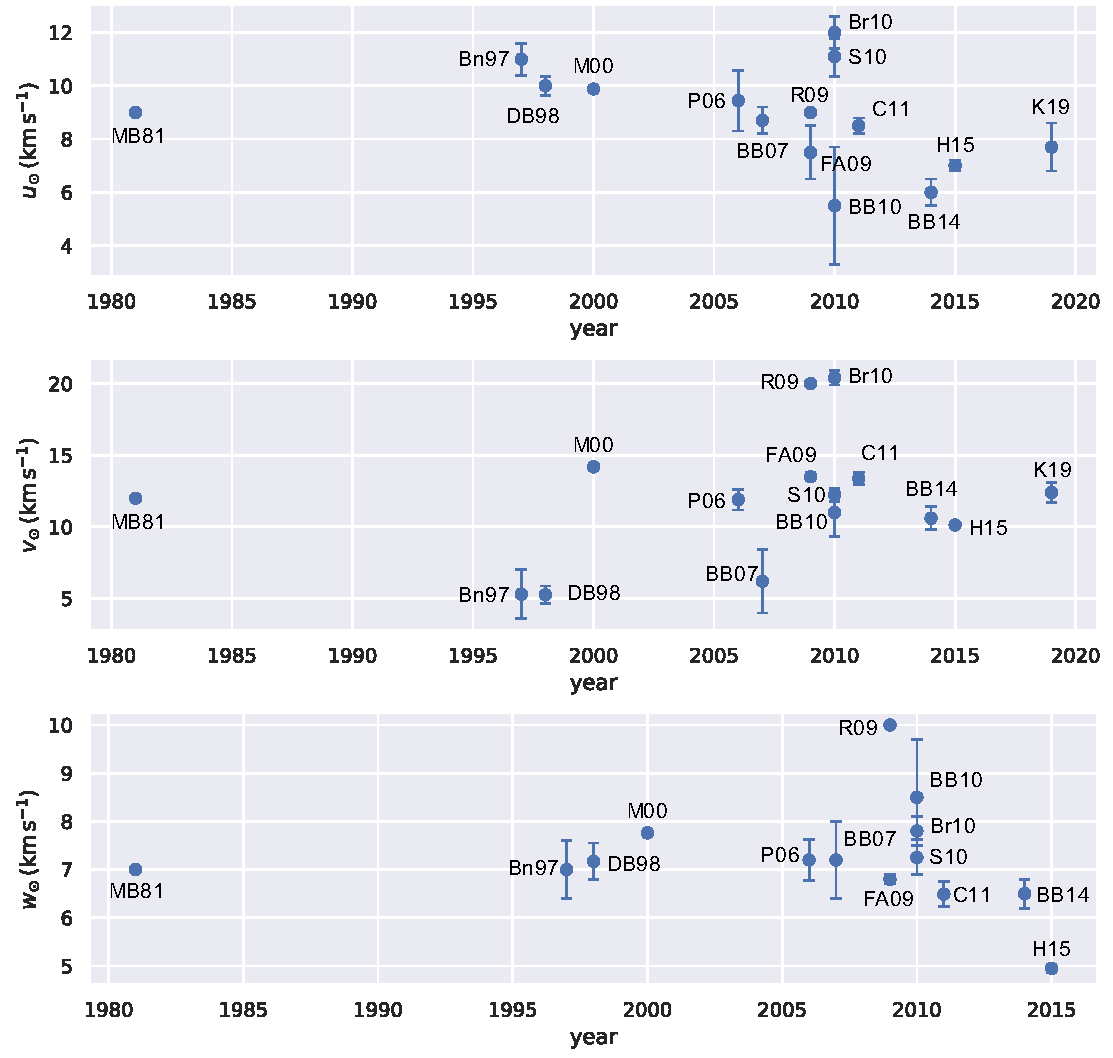
\includegraphics[width=13cm]{fig/UVW.pdf}
	\caption{先行研究の太陽運動の値のプロット。ラベルについては表\ref{table2}を参照。}
	\label{fig:uvw}
\end{figure*}
% 2 Oort-Lindbladモデルと観測方程式 (仮)
% 2.1 速度分散の無い系の太陽運動と銀河速度場 ← 宮本ノートや藤田修論を参考に書く
% 2.1.1 Oort-Lindbladモデル ← A, B, C, Kの導出と物理的意味
% 2.1.2 観測方程式 ← 従来のもの

% 2.2 速度分散を考慮した場合への拡張 ← Olling & Dehnenを参考に書く
% 2.2.1 従来のOort-Lindbladモデルの問題点 ← ここにYu & Liu の年齢速度分散関係の図も載せるとよい。
% 2.2.2 asymmetric drift ← 導出&物理的解釈を書く
% 2.2.3 asymmetric driftを考慮した観測方程式



% Chap. 2 Oort-Lindbladモデルと観測方程式
% p.11にOlling & Dehnen 2002の表 (A, B, C, Kの表記の違い) を載せていますが、
% この表記の表は載せる必要がありますか?

% 式(2.30a,b)の導出と、それを用いたAa, Baとvaの関係の評価 (すぐ下に文章で書いてある) は、
% 単にOlling & Dehnenの翻訳ではなく、ちゃんと自分の言葉で書きましょう。
% (そもそもここの文章に書いてある近似式は自分で導出しましたか?)
% この関係は、模擬データの解析結果の解釈の部分でも利用する近似式だと思います。


\chapter{Oort-Lindbladモデルと観測方程式 \label{chapTheory}}
この章では、本研究で用いているOort-Lindbladモデルと、実際に観測データにこのモデルを適用する観測方程式の説明をする。まず、速度分散の無い系でのOort-Lindbladモデルと観測方程式について説明する。その後、従来のOort-Lindbladモデルの問題点と、速度分散を考慮した場合に考えるべき効果に加えて、そのような場合に拡張した観測方程式の説明をする。

ここで、本章で用いる文字の表記法を表\ref{notation}に整理しておく。
\begin{table}
\begin{center}
%\scalebox{0.5}
%\scriptsize
%\footnotesize
%\small
\begin{tabular}{c|l} \hline
 \rowcolor{LightCyan}
 文字 & 文字が示す意味\\
 \hline
 $\pmb{R}$ & 銀河中心を原点とするときの星の位置ベクトル\\
 \hline
 $\pmb{R_{\odot}}$ & 銀河中心を原点とするときの太陽の位置ベクトル\\
 \hline
 $\pmb{r}$ & 太陽を原点とするときの星の位置ベクトル ($\pmb{r}=\pmb{R}-\pmb{R_{\odot}}$)\\
 \hline
 $\pmb{v}_*$ & 銀河中心を静止基準とするときの星の速度\\
 \hline
 $\pmb{v}_{\odot}$ & 銀河中心を静止基準とするときの太陽の速度\\
 \hline
 \multirow{2}{*}{$\pmb{V}(\pmb{R})$} & 銀河中心を静止基準とする。このときの星の集団に\\
   & 速度分散があるときの位置$\pmb{R}$での系統速度 \tabularnewline[\doublerulesep]
 \hline
 \multirow{2}{*}{$\pmb{V}_{\mathrm{c}}(\pmb{R})$} & 銀河中心を静止基準とする。このときの星の集団に速度分散がない、\\
   & すなわち星が円運動をしているときの位置$\pmb{R}$での系統速度 \tabularnewline[\doublerulesep]
 \hline
 \multirow{2}{*}{$\pmb{v}_{\mathrm{p}}$} & 星の特異速度 (銀河中心を静止基準とするときの星の速度$\pmb{v}_*$から\\
   & 星の位置での系統速度$\pmb{V}(\pmb{R})$を引いたもの) \tabularnewline[\doublerulesep]
 \hline
 \multirow{2}{*}{$\pmb{v}_{\mathrm{p},\odot}$} & 太陽の特異速度 (銀河中心を静止基準とするときの太陽の速度$\pmb{v}_{\odot}$から\\
   & 太陽の位置での系統速度$\pmb{V}(\pmb{R_{\odot}})$を引いたもの) \tabularnewline[\doublerulesep]
 \hline
 $\pmb{v}_{\mathrm{rel}}$ & 太陽を静止基準とするときの星の速度\\
 \hline
 \multirow{2}{*}{$(x,y,z)$} & 太陽を原点とした直交座標系。それぞれ銀経$l=0^{\circ}$かつ銀緯$b=0^{\circ}$、\\
    & $l=90^{\circ}$かつ$b=0^{\circ}$、$b=90^{\circ}$の向きの軸。 \tabularnewline[\doublerulesep]
 \hline
 $(R,\phi,z)$ & 銀河中心を原点とした円筒座標系\\
 \hline
 $\sigma_R、\sigma_{\phi}、\sigma_z$ & 円筒座標系で表された速度の速度分散\\
 \hline
 \multirow{3}{*}{$A_{\mathrm{c}}、B_{\mathrm{c}}、C_{\mathrm{c}}、K_{\mathrm{c}}$} & 星の集団が速度分散を持たずに銀河中心の周りを運動、\\
    & すなわち円運動をしているときのオールト定数。\\
    & それぞれ銀河回転方向の剪断成分、回転成分、動径方向の剪断成分、発散成分。 \tabularnewline[\doublerulesep] 
 \hline
 $A、B、C、K$ & 星の集団が速度分散を持って運動しているときの系統運動のオールト定数\\
 \hline
 $A_{\mathrm{a}}、B_{\mathrm{a}}、C_{\mathrm{a}}、K_{\mathrm{a}}$ & オールト定数$A_{\mathrm{c}}、B_{\mathrm{c}}、C_{\mathrm{c}}、K_{\mathrm{c}}$がasymmetric driftの効果によってずれる値。\\
 \hline
 $U_{\odot}、V_{\odot}、W_{\odot}$ & 太陽の特異速度の動径方向、銀河回転方向、銀河北極方向成分\\
 \hline
 $\Phi$ & 重力ポテンシャル\\
 \hline
 $v_l、v_b、v_{\mathrm{los}}$ & 銀河座標系での速度。それぞれ銀経方向、銀緯方向、視線方向。\\
 \hline
 $\mu_l、\mu_b$ & 銀河座標系での固有運動。それぞれ銀経方向、銀緯方向。\\
 \hline
 $v_{\mathrm{a}}$ & Str\"{o}mbergの関係により導かれるasymmetric drift速度\\
 \hline
 $\Omega_{g,\odot}$ & 銀河中心を静止基準とするときの太陽系の銀河回転方向の角速度\\
 \hline
\end{tabular} \label{notation}
\vspace{3mm}
\caption{本論文で用いる各パラメータや座標系の定義をまとめた表}
\end{center}
\end{table}

\section{速度分散の無い系の太陽運動と銀河速度場} % 宮本ノートや藤田修論を参考に書く
この節では、速度分散の無い系での太陽運動とOort-Lindbladモデル、銀河系の速度場について説明する。太陽系近傍の星の速度は、系統速度 (systematic velocity) と特異速度 (peculiar velocity) とに分けることができ、太陽運動とは太陽の特異速度のことを意味する。系統速度とは、銀河系内のある位置だけで決まる一意的な速度のことであり、その位置の周辺の星の集団の平均速度場である。特異速度とは、系統速度と1つ1つの星の速度との差であり、銀河系の星は基本的には円軌道ではないため、それぞれの星ごとに特異速度を持つ。太陽の位置で系統速度で動く点は局所静止基準 (LSR; Local Standard of Rest) と呼ばれ、太陽系の位置で銀河系中心を中心として円運動をしていると仮定される。本論文では、太陽運動は$\pmb{v}_{\mathrm{p},\odot} = (U_{\odot},V_{\odot},W_{\odot})$で表す。$(U_{\odot},V_{\odot},W_{\odot})$はそれぞれ銀河中心方向、銀河回転方向、銀河北極方向と定義する (図\ref{fig:SolarMotion})。
\begin{figure*}[htbp]
\begin{center}
	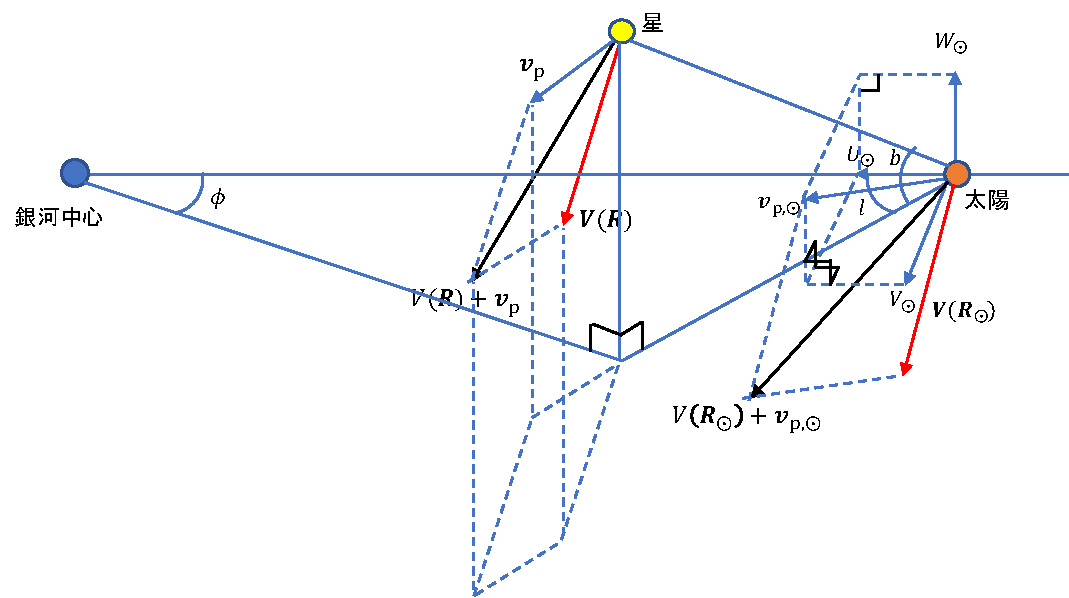
\includegraphics[width=14cm]{fig/SolarMotion.pdf}
	\caption{銀河系円盤を回転する星と太陽の系統速度$\pmb{V}(\pmb{R})、\pmb{V}(\pmb{R_{\odot}})$、星と太陽の特異速度$\pmb{v}_{\mathrm{p}}、\pmb{v}_{\mathrm{p}_\odot}$をベクトルで書いたときの例。赤色の矢印は系統速度、青色の矢印は特異速度、黒色の矢印は系統速度と特異速度を足した速度を表している。図のように速度ベクトルを足すことで、銀河中心に対する星の速度は$\pmb{V}(\pmb{R}_{\odot}) + \pmb{v}_{\mathrm{p},\odot}$、銀河中心に対する太陽の速度は$\pmb{V}(\pmb{R}) + \pmb{v}_{\mathrm{p}}$と表せる。ここでは簡単のために$\pmb{V}(\pmb{R})、\pmb{V}(\pmb{R}_{\odot})、\pmb{v}_{\mathrm{p}}$は銀緯$b=0^{\circ}$面内にあることにする。$(U_{\odot},V_{\odot},W_{\odot})$は太陽運動の特異速度であり、それぞれ銀河中心方向、銀河回転方向、銀河北極方向のベクトルであり、直交座標系に沿ったベクトルである。}
	\label{fig:SolarMotion}
\end{center}
\end{figure*}

%%%%%%%%%%%%%%%%%%%%%%%%%%%%%%%%%%%%%%%%%%%%%%%%%%%%%%%%%%%%%%%%%%%%%%%%
%%%%%%%%%%%%%%%%%%%%%%%%%%%%%%%%%%%%%%%%%%%%%%%%%%%%%%%%%%%%%%%%%%%%%%%%
%%%%%%%%%%%%%%%%%%%%%%%%%%%%%%%%%%%%%%%%%%%%%%%%%%%%%%%%%%%%%%%%%%%%%%%%

\subsection{Oort-Lindbladモデル} % A, B, C, Kの導出と物理的意味
Oort-Lindbladモデルとは、\cite{Oort1927b}, \cite{Lindblad1927}, \cite{Chandra42}らによって構築された太陽近傍の銀河系速度場を記述するモデルである。ここでは、このモデルの導出とパラメータの説明をする。

銀河系中心に原点を置く静止座標系を考える。このときの太陽近傍星と太陽の速度をそれぞれ$\pmb{v}_{*}、\pmb{v}_{\odot}$とする。また、位置$\pmb{R}$での系統速度を$\pmb{V}(\pmb{R})$、太陽近傍星と太陽の特異速度をそれぞれ$\pmb{v}_{\mathrm{p}}、\pmb{v}_{\mathrm{p}_\odot}$とする (図\ref{fig:SolarMotion})。
また、2次元面 (銀河円盤面) に運動を限定する。すなわち、銀緯$b=0^{\circ}$の面で考える。このとき、
\begin{align}
\begin{aligned}
	\pmb{v}_* &= \pmb{V}(\pmb{R}) + \pmb{v}_{\mathrm{p}} \\
	\pmb{v}_{\odot} &= \pmb{V}(\pmb{R}_{\odot}) + \pmb{v}_{\mathrm{p},\odot}
\end{aligned}
\end{align}
と書ける。太陽を静止基準とするときの太陽近傍星の速度$\pmb{v}_{\rm rel}$は、星の特異速度を無視すると、
\begin{align}
\begin{aligned}
	\pmb{v}_{\rm rel} &= \pmb{v}_* - \pmb{v}_{\odot} \\
	&= [\pmb{V}(\pmb{R}) - \pmb{V}(\pmb{R}_{\odot})] - \pmb{v}_{\mathrm{p},\odot}
\end{aligned}
\end{align}
となる。ここで、太陽に対する星の位置ベクトルを$\pmb{r} = \pmb{R} - \pmb{R}_{\odot}$とする。$\pmb{R}、\pmb{R}_{\odot}$はそれぞれ星、太陽の位置ベクトルである。星と太陽との距離が星と銀河中心との距離$\pmb{x}$に対して十分小さい$(|\pmb{r}| = |\pmb{R}-\pmb{R}_{\odot}| \ll |\pmb{x}|)$と仮定すると、太陽にいる観測者から見た銀河系内でのある位置$\pmb{R}$での系統速度はテイラー展開することができる。このとき、太陽を中心とした直交座標系を考え、$x$軸、$y$軸はそれぞれ銀経$l=0^{\circ}、90^{\circ}$の方向とすると、
\begin{align}
\begin{aligned}
	\pmb{v}_{\rm rel} &\simeq \pmb{H} \cdot \pmb{r} - \pmb{v}_{\mathrm{p},\odot} + \mathcal{O}(\pmb{r}^2) \label{eq:1}
\end{aligned}
\end{align}
と書けるから、
\begin{align}
\begin{aligned}
	\pmb{H} \simeq
	\left. \frac{\partial \pmb{V}(\pmb{R})}{\partial \pmb{R}} \right|_{\pmb{R}=\pmb{R}_{\odot}}
	&=
	\left(
	\begin{array}{cc}
	 	\cfrac{\partial V_x}{\partial x} & \cfrac{\partial V_x}{\partial y}\\
		\cfrac{\partial V_y}{\partial x} & \cfrac{\partial V_y}{\partial y}\\
	\end{array}
	\right) \\
	&=
	\left(
	\begin{array}{cc}
	 	K+C & A-B\\
		A+B & K-C\\
	\end{array}
	\right)
\end{aligned} \label{eq2}
\end{align}
となる。ここで、$A、B、C、K$を以下のように定義すると
\begin{subequations}
\begin{align}
	A &=\frac{1}{2}\left(\frac{\partial V_y}{\partial x} + \frac{\partial V_x}{\partial y}\right)_{R=R_{\odot}} \label{eq2.1a}\\
	B &=\frac{1}{2}\left(\frac{\partial V_y}{\partial x} - \frac{\partial V_x}{\partial y}\right)_{R=R_{\odot}} \label{eq2.1b}\\
	C &=\frac{1}{2}\left(\frac{\partial V_x}{\partial x} - \frac{\partial V_y}{\partial y}\right)_{R=R_{\odot}} \label{eq2.1c}\\
	K &=\frac{1}{2}\left(\frac{\partial V_x}{\partial x} + \frac{\partial V_y}{\partial y}\right)_{R=R_{\odot}} \label{eq2.1d}
\end{align} \label{eq2.1}
\end{subequations}
となる。

パラメータ$A,B,C,K$はオールト定数と呼ばれる。これらは太陽近傍星の運動学が力学的に冷たい系である場合の平均速度場を表すパラメータであり、それぞれ銀河回転方向の剪断成分、回転成分、動径(太陽と銀河中心を結ぶ方向)方向の剪断成分、発散成分を示す。式(\ref{eq2.1})は直交座標系で表したオールト定数であるが、一般的にはオールト定数は円筒座標系$(R,\phi)$ (座標系の取り方は図(\ref{fig:coordinates})を参照)で表される(\cite{Chandra42})。そこで、直交座標系から円筒座標系への座標変換をする。
\begin{align}
\begin{cases}
	x &= R_{\odot} - R\cos{\phi}\\
	y &= R\sin{\phi}
\end{cases}
\end{align}

\begin{align}
\begin{cases}
	R &= \sqrt{(R_{\odot}-x)^2 + y^2 }\\
	\phi &= \arctan{\cfrac{y}{R_{\odot}-x}}
\end{cases}
\end{align}

\begin{align}
\begin{aligned}
	\left(
	\begin{array}{c}
	 	V_x\\
		V_y\\
	\end{array}
	\right)
	&=
	\left(
	\begin{array}{cc}
	 	\cos{\phi} & \sin{\phi}\\
		-\sin{\phi} & \cos{\phi}\\
	\end{array}
	\right)
	\left(
	\begin{array}{c}
	 	-V_R\\
		V_{\phi}\\
	\end{array}
	\right) \\
	&=
	\left(
	\begin{array}{c}
	 	-\cos{\phi}\ V_R + \sin{\phi}\ V_{\phi}\\
		\sin{\phi}\ V_R + \cos{\phi}\ V_{\phi}\\
	\end{array}
	\right)
\end{aligned}
\end{align}
から、
\begin{align}
\begin{cases}
	\cfrac{\partial R}{\partial x} &= \cfrac{x-R_{\odot}}{R} = -\cos{\phi} \\[2mm]
	\cfrac{\partial R}{\partial y} &= \cfrac{y}{R} = \sin{\phi} \\[2mm]
	\cfrac{\partial \phi}{\partial x} &= \cfrac{y}{(R_{\odot}-x)^2 + y^2} = \cfrac{\sin{\phi}}{R} \\[2mm]
	\cfrac{\partial \phi}{\partial y} &= \cfrac{R_{\odot}-x}{(R_{\odot}-x)^2 + y^2} = \cfrac{\sin{\phi}}{R}
\end{cases} \label{eq139}
\end{align}
となる。太陽の位置で座標変換をするために式\ref{eq139}に太陽の位置$(R,\phi)=(R_{\odot},0)$を代入すると
\begin{align}
\begin{cases}
	\cfrac{\partial R}{\partial x} &= -1 \\[2mm]
	\cfrac{\partial R}{\partial y} &= 0 \\[2mm]
	\cfrac{\partial \phi}{\partial x} &= 0 \\[2mm]
	\cfrac{\partial \phi}{\partial y} &= \cfrac{1}{R_{\odot}}
\end{cases} \label{eq161}
\end{align}
となるから、偏微分を$R=R_{\odot}$近傍で行うとき、式(\ref{eq161})を用いて
\begin{align}
\begin{cases}
	\left.\cfrac{\partial V_x}{\partial x}\right|_{R=R_{\odot}} &= \cfrac{\partial R}{\partial x}\cfrac{\partial V_x}{\partial R} + \cfrac{\partial \phi}{\partial x}\cfrac{\partial V_x}{\partial \phi} = \cfrac{\partial V_R}{\partial R} \\[2mm]
	\left.\cfrac{\partial V_x}{\partial y}\right|_{R=R_{\odot}} &= \cfrac{\partial R}{\partial y}\cfrac{\partial V_x}{\partial R} + \cfrac{\partial \phi}{\partial y}\cfrac{\partial V_x}{\partial \phi} = -\cfrac{1}{R_{\odot}}\left(-\cfrac{\partial V_R}{\partial \phi} + V_{\phi}\right)\\[2mm]
	\left.\cfrac{\partial V_y}{\partial x}\right|_{R=R_{\odot}} &= \cfrac{\partial R}{\partial x}\cfrac{\partial V_y}{\partial R} + \cfrac{\partial \phi}{\partial x}\cfrac{\partial V_y}{\partial \phi} = -\cfrac{\partial V_{\phi}}{\partial R}\\[2mm]
	\left.\cfrac{\partial V_y}{\partial y}\right|_{R=R_{\odot}} &= \cfrac{\partial R}{\partial y}\cfrac{\partial V_y}{\partial R} + \cfrac{\partial \phi}{\partial y}\cfrac{\partial V_y}{\partial \phi} = \cfrac{1}{R_{\odot}}\left(V_R + \cfrac{\partial V_{\phi}}{\partial \phi}\right)
\end{cases}
\end{align}
となる。以上の式を使用し、オールト定数を円筒座標系で書き直すと
\begin{subequations}
\begin{align}
	A &=\frac{1}{2}\left( \frac{V_{\phi}}{R_{\odot}} - \frac{\partial V_{\phi}}{\partial R} - \frac{1}{R_{\odot}}\frac{\partial v_{R}}{\partial \phi} \right)_{R=R_{\odot}} \label{eq2.5a}\\
	B &=\frac{1}{2}\left( -\frac{V_{\phi}}{R_{\odot}} - \frac{\partial V_{\phi}}{\partial R} + \frac{1}{R_{\odot}}\frac{\partial v_{R}}{\partial \phi} \right)_{R=R_{\odot}} \label{eq2.5b}\\
	C &=\frac{1}{2}\left( -\frac{v_{R}}{R_{\odot}} + \frac{\partial V_R}{\partial R} - \frac{1}{R_{\odot}}\frac{\partial V_{\phi}}{\partial \phi} \right)_{R=R_{\odot}} \label{eq2.5c}\\
	K &=\frac{1}{2}\left( \frac{v_{R}}{R_{\odot}} + \frac{\partial V_R}{\partial R} + \frac{1}{R_{\odot}}\frac{\partial V_{\phi}}{\partial \phi} \right)_{R=R_{\odot}} \label{eq2.5d}
\end{align} \label{eq2.5}
\end{subequations}
のようになる。


\begin{figure*}[htbp]
\begin{center}
	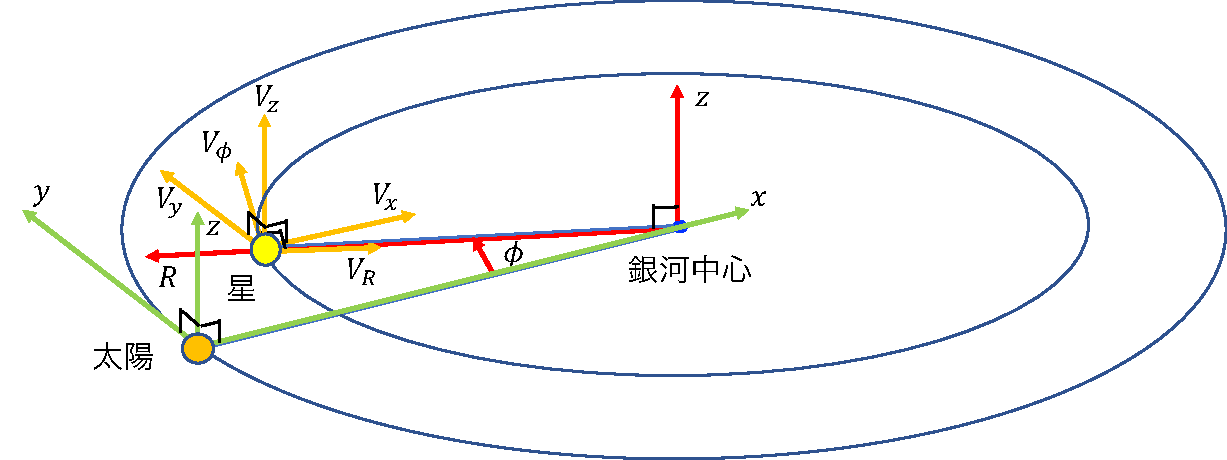
\includegraphics[width=10cm]{fig/Coordinates.pdf}
	\caption{天の川銀河を北銀極方向から斜めに眺め下ろした図。緑線は太陽系を中心とした直交座標系$(x,y,z)$、赤線は銀河系中心を中心とした円筒座標系$(R,\phi,z)$、黄線は直交座標系での星の速度ベクトル$(V_x,V_y,V_z)$を表している。}
	\label{fig:coordinates}
\end{center}
\end{figure*}

軸対称な系を考えると、速度分散が非常に小さいときの系統速度は円軌道に近似できるため、このとき$V_{\phi}=V_{\mathrm{c}}$となる。これに加えて天の川銀河が膨張も収縮もしていないと仮定すると$C=K=0$となり、
%\footnote[1]{しかしながら、$C$と$K$がゼロであることは銀河系ポテンシャルが軸対称になる上で必要ではないことに注意しなければならない。代わりに太陽が楕円ポテンシャルの主軸の近くに位置する可能性がある。(\cite{KT1994})}
\begin{subequations}
\begin{align}
	A_{\mathrm{c}} &=\frac{1}{2}\left( \frac{V_{\mathrm{c}}}{R} - \frac{\partial V_{\phi}}{\partial R} \right)_{R=R_{\odot}} \\
	B_{\mathrm{c}} &=\frac{1}{2}\left( -\frac{V_{\mathrm{c}}}{R} - \frac{\partial V_{\phi}}{\partial R} \right)_{R=R_{\odot}}
\end{align} \label{ABsym}
\end{subequations}
はオールトによって実際に得られた式である。$R_{\odot}$は太陽から銀河中心までの距離を表す。円軌道の速度$V_{\mathrm{c}}$は中心力と遠心力のつりあいから$V_{\mathrm{c}}^2=R \partial\ \Phi/\partial R$を持ち、オールト定数の測定は銀河系ポテンシャル$\Phi$の直接的な制限をすることになる。例えば、調和振動子ポテンシャル$(\Phi \propto R^2)$では、
\begin{align}
\begin{aligned}
    V_{\mathrm{c}} = R \cfrac{\partial \Phi}{\partial R} = 2R^2 \propto R^2 \to V_{\mathrm{c}} \propto R
\end{aligned}
\end{align}
から、
\begin{subequations}
\begin{align}
	A_{\mathrm{c}} &\propto\frac{1}{2}\left( \frac{R}{R} - \frac{\partial R}{\partial R} \right) = 0\\
	B_{\mathrm{c}} &\propto \frac{1}{2}\left( -\frac{R}{R} - \frac{\partial R}{\partial R} \right) = 1
\end{align}
\end{subequations}
となる。このとき、銀河回転は剛体回転となり、$B_{\mathrm{c}}$は銀河の回転周波数と等しくなる。また、回転曲線が平坦なとき$(V_{\mathrm{c}}=\mathrm{const})$には、定数$a$を用いて$V_{\mathrm{c}} = a$とすると、
\begin{subequations}
\begin{align}
	A_{\mathrm{c}} &=\frac{1}{2}\left( \frac{a}{R} - \frac{\partial a}{\partial R} \right) = \frac{1}{2}\frac{a}{R}\\
	B_{\mathrm{c}} &=\frac{1}{2}\left( -\frac{a}{R} - \frac{\partial a}{\partial R} \right) = -\frac{1}{2}\frac{a}{R}
\end{align}
\end{subequations}
から$A_{\mathrm{c}} = -B_{\mathrm{c}}$となる。さらに、全質量が銀河系中心付近に集中してケプラーポテンシャルとなっているとき$(V_{\mathrm{c}} \propto R^{-1/2})$には、中心力$F$、重力定数$G$、星の質量$M$を用いると、$F = \dfrac{GM}{R^2} = \dfrac{V_{\mathrm{c}}^2}{R}$から
\begin{align}
\begin{aligned}
    V_{\mathrm{c}}^2 = \frac{GM}{R} \to V_{\mathrm{c}} \propto R^{-1/2}
\end{aligned}
\end{align}
となるため、
\begin{subequations}
\begin{align}
	A_{\mathrm{c}} &\propto \frac{1}{2}\left( \frac{R^{-1/2}}{R} - \frac{\partial R^{-1/2}}{\partial R} \right) = \frac{3}{4}R^{-3/2}\\
	B_{\mathrm{c}} &\propto \frac{1}{2}\left( -\frac{R^{-1/2}}{R} - \frac{\partial R^{-1/2}}{\partial R} \right) = -\frac{1}{4}R^{-3/2}
\end{align}
\end{subequations}
から$A_{\mathrm{c}}=-3B_{\mathrm{c}}$となる。\cite{Oort1927b}は、不定性は大きいものの、視線速度と固有運動から$A\approx 19\,\mathrm{km\,s^{-1} kpc^{-1}}, B\approx -24\,\mathrm{km\,s^{-1} kpc^{-1}}$という値を得た。オールトはこの結果から銀河ポテンシャルは調和振動子ポテンシャルやこれは、まだ天の川銀河が回転していることが定着していなかった頃のことである。このオールトの研究結果は天の川銀河が回転していることの明確な証拠となり、天の川銀河は剛体回転しているというLindbladの提案を棄却した。


%%%%%%%%%%%%%%%%%%%%%%%%%%%%%%%%%%%%%%%%%%%%%%%%%%%%%%%%%%%%%%%%%%%%%%%%
%%%%%%%%%%%%%%%%%%%%%%%%%%%%%%%%%%%%%%%%%%%%%%%%%%%%%%%%%%%%%%%%%%%%%%%%
%%%%%%%%%%%%%%%%%%%%%%%%%%%%%%%%%%%%%%%%%%%%%%%%%%%%%%%%%%%%%%%%%%%%%%%%

\subsection{観測方程式 \label{観測方程式}}
ここで、銀河中心を基準とした星の速度を$\delta\pmb{V}$、そして$\delta\pmb{V}$の$x、y$成分を$\delta V_x、\delta V_y$とすると、次のように書ける。
\begin{align}
\begin{aligned}
	\delta\pmb{V} =
	\left(
	\begin{array}{c}
	 	\delta V_x\\
		\delta V_y
	\end{array}
	\right)
	=
	\pmb{H} \cdot \pmb{r}
	=&
	\left(
	\begin{array}{cc}
	 	K+C & A-B\\
		A+B & K-C
	\end{array}
	\right)
	\cdot
	\left(
	\begin{array}{c}
	 	x\\
		y
	\end{array}
	\right)\\
	=&
	\left(
	\begin{array}{c}
	 	(K+C)x + (A-B)y\\
		(A+B)x + (K-C)y
	\end{array}
	\right)
\end{aligned} \label{eq266}
\end{align}

簡単のためにテイラー展開の2次の項$\mathcal{O}(\pmb{r}^2)$は無視している。銀経$l$の位置を太陽に対して速度$(U,V)$で運動している星は視線速度$v_d$、接線速度$v_l$で観測される (図\ref{fig:OD03})。
ある星と太陽との距離を$d$、銀経を$l$とすると、$x = d\cos l,y = d \sin l$と書ける。式(\ref{eq266})を用いると、
\begin{align}
\begin{aligned}
	v^*_d &= \frac{1}{d} \pmb{r} \cdot \delta\pmb{V}
	= \frac{1}{d}(x\delta V_x + y\delta V_y) \\
	&= \frac{1}{d} [(K+C)x^2 + (K-C)y^2 + 2Axy] \\
	&= \frac{1}{d} [K(x^2 + y^2) + C(x^2 - y^2) + 2Axy] \\
	&= d(K + C\cos2l + A\sin2l)
\end{aligned} \label{vd}
\end{align}
となる。ここで、$v^*_d$は太陽の位置での系統速度$\pmb{V}(\pmb{R}_{\odot})$で運動すると仮定する点 (LSR)を静止基準とするとき、さらに星が$b=0^{\circ}$の2次元面内を運動していると仮定するときの視線速度である。つまり、LSRを静止基準とするときの星の視線速度を銀河円盤面 ($b=0^{\circ}$面)に投影した速度である。

式(\ref{vd})から、太陽系近傍の星の視線速度と銀経$l$、距離$d$からオールト定数$A、C、K$を決定することができることがわかる。一方オールト定数$B$は星の固有運動から求めることができる。太陽の位置での系統速度$\pmb{V}(\pmb{R}_{\odot})$で運動すると仮定する点 (LSR)を静止基準とするときの星の接線速度$v^*_l$は、式(\ref{eq266})を用いて
\begin{align}
\begin{aligned}
	v^*_l &= \frac{1}{d}(\pmb{r} \times \delta\pmb{V})_z = \frac{1}{d}(x\delta V_y - y\delta V_x)\\
	&= \frac{1}{d}[B(x^2 + y^2) + A(x^2 - y^2) - 2Cxy] \\
	&= d(B + A\cos2l - C \sin2l)
\end{aligned}
\end{align}
となる。銀緯$b=0$面の星を見ているとき、太陽系の特異速度の視線速度成分、接線速度成分を$v_{\odot,d}、v_{\odot,l}$と書くと、
\begin{align}
\begin{aligned}
	\left(
	\begin{array}{c}
	 	v_{\odot,d}\\
		v_{\odot,l}\\
	\end{array}
	\right)
	&=
	\left(
	\begin{array}{cc}
	 	\cos l & \sin l\\
		-\sin l & \cos l\\
	\end{array}
	\right)
	\left(
	\begin{array}{c}
	 	U_{\odot}\\
		V_{\odot}\\
	\end{array}
	\right) \\
	&=
	\left(
	\begin{array}{c}
	 	U_{\odot} \cos l + V_{\odot} \sin l\\
		-U_{\odot} \sin l + V_{\odot} \cos l\\
	\end{array}
	\right)
\end{aligned}
\end{align}
となるから、星が$b=0^{\circ}$の2次元面内を運動していると仮定するとき、太陽を静止基準とするときの星の視線速度と接線速度$v_d、v_l$は
\begin{subequations}
\begin{align}
    v_d &= v^*_d - v_{\odot,d} =  d(K+A\sin{2l}+C\cos{2l}) -V_{\odot}\sin{l} - U_{\odot}\cos{l} \label{eq:6} \\
    v_l &= v^*_l - v_{\odot,l} = d(B-C\sin{2l}+A\cos{2l}) + U_{\odot}\sin{l} - V_{\odot}\cos{l} \label{eq:7}
\end{align}
\end{subequations}
と表される。


実際には天の川銀河は円盤面上に全ての星が存在するような2次元の構造ではなく、星が円盤面から離れたところにも存在する3次元であるため、$v_d,v_l$の式を直接的には使えない。したがって、銀河円盤面の外の星を一般化するために以下の式を使う。
\begin{subequations}
\begin{align}
	\varpi &= d^{-1} \cos b \\
	v_{\mathrm{los}} &= v_d \cos b + V_z \sin b\\
	\mu^*_l &= \varpi v_l \\
	\mu_b &= \varpi(V_z \cos b - v_d \sin b)
\end{align} \label{OD03}
\end{subequations}
ここで、$\mu^*_l \equiv \mu_l \cos b$ (観測で直接得られる値)である。上式の表記については図(\ref{fig:OD03})を参照されたい。
\begin{figure*}[htbp]
\begin{center}
	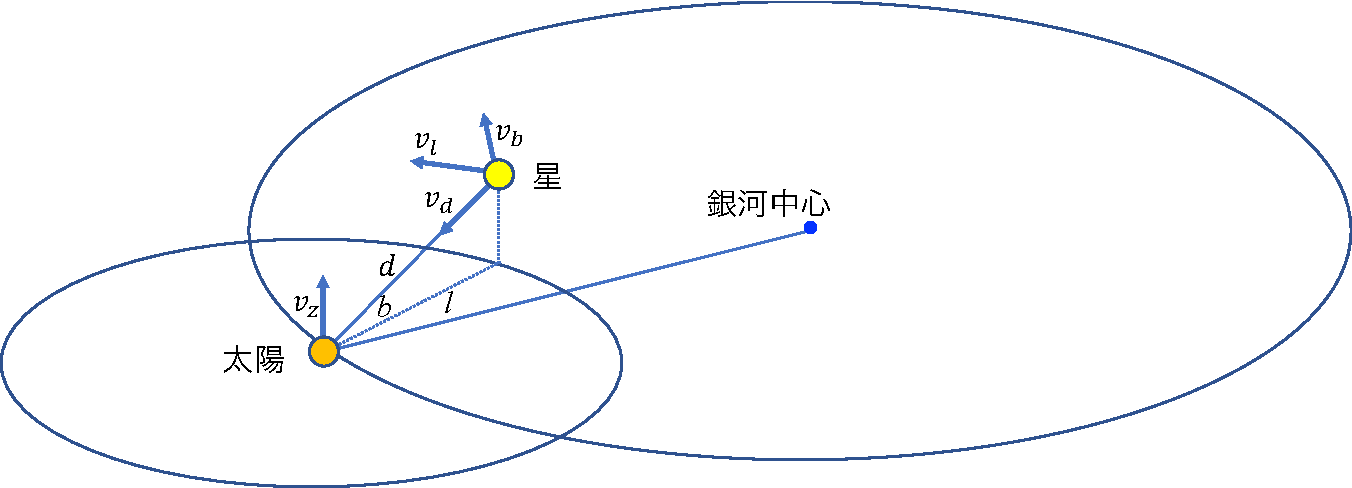
\includegraphics[width=10cm]{fig/figOD2003.pdf}
	\caption{式(\ref{OD03})、式(\ref{Q})で使われている各パラメータが示す量。$l、b$はそれぞれ銀経、銀緯。$a$は星の銀河円盤面での位置と銀河中心、太陽の位置とを結んだときの角度。$d$は星と太陽との距離。$v_l,v_b,v_{\mathrm{los}}$はそれぞれ星の銀経方向、銀緯方向、視線方向の速度。実際の観測量は3次元の速度を持っているため、2次元モデルを使うことができるように円盤から離れた星の位置・速度を円盤面に投影する。$v^*_d$は、太陽の位置での系統速度$\pmb{V}(\pmb{R}_{\odot})$で運動すると仮定する点 (LSR)を静止基準とするときの、ある星の視線速度を銀河円盤面 ($b=0^{\circ}$面)に投影した速度である。$v^*_l$は、LSRを静止基準とするときのある星の接線速度である。}
	\label{fig:OD03}
\end{center}
\end{figure*}
Oort-Lindbladモデルにおける$\mu^*_l$を$\mu^{*,\mathrm{OL}}_l$、$\mu_b$を$\mu^{\mathrm{OL}}_b$、$v_{\mathrm{los}}$を$v^{\mathrm{OL}}_{\mathrm{los}}$と書くことにすると、
\begin{subequations}
\begin{align}
	\mu^{*,\mathrm{OL}}_l(l_i,b_i,\varpi_i) &= (A\cos2l_i - C\sin2l_i + B)\cos b_i + \varpi_i(U_{\odot}\sin l_i - V_{\odot}\cos l_i) \\
	\mu^{\mathrm{OL}}_b(l_i,b_i,\varpi_i) &= -(A\sin2l_i + C\cos2l_i + K)\sin b_i \cos b_i \nonumber \\
	                          & \hspace{2cm} + \varpi_i[(U_{\odot}\cos l_i + V_{\odot} \sin l_i)\sin b_i - W_{\odot} \cos b_i] \\
	v^{\mathrm{OL}}_{\mathrm{los}}(l_i,b_i,\varpi_i) &= (K + C\cos2l_i + A\sin2l_i)\varpi_i^{-1}  \cos^2 b_i \nonumber\\
	                      & \hspace{2cm} - [(U_{\odot}\cos l_i + V_{\odot} \sin l_i)\cos b_i + W_{\odot} \sin b_i]
\end{align} \label{ObsEq}
\end{subequations}
となり、これが基本的な観測方程式となる。ここで、OLの添字はOort-Lindbladモデルの式であることを示す。また、添字$i$は星ごとの観測量であることを示す。

実際に解析する際の観測方程式の使用方法について簡単に説明する。例えば観測データの中の$i$番目の星が銀経$l_i$、銀緯$b_i$、年周視差$\varpi_i$、固有運動$\mu_ {l,i}$とその誤差$e_{\mu_ {l,i}}$を持っているとき、$\mu_{l,i}$が標準偏差$e_{\mu_ {l,i}}$の正規分布の確率分布で$l_i、b_i、\varpi_i$の関数で書ける$\mu^{*,\mathrm{OL}}_l(l_i,b_i,\varpi_i)$と一致すると仮定する。これにより、式(\ref{ObsEq})の中の$\mu^{*,\mathrm{OL}}_l(l_i,b_i,\varpi_i)$の式に含まれているパラメータ$A、B、C、U_{\odot}、V_{\odot}$が得られることになる。同様に$\mu_{b,i}$と$\mu^{\mathrm{OL}}_b(l_i,b_i,\varpi_i)$とでフィッティングをすることでパラメータ$A、C、K、U_{\odot}、V_{\odot}、W_{\odot}$が得られ、$v^{\mathrm{OL}}_{\mathrm{los}}(l_i,b_i,\varpi_i)$も同様にパラメータを得られる。先行研究では固有運動の式2つのみでフィッティングをしているものもあるが、可能な限り正確にパラメータ推定を行うためには式1つや2つよりも式3つで行う方が良いため、本論文では3つの式を用いて解析している。

%%%%%%%%%%%%%%%%%%%%%%%%%%%%%%%%%%%%%%%%%%%%%%%%%%%%%%%%%%%%%%%%%%%%%%%%
%%%%%%%%%%%%%%%%%%%%%%%%%%%%%%%%%%%%%%%%%%%%%%%%%%%%%%%%%%%%%%%%%%%%%%%%
%%%%%%%%%%%%%%%%%%%%%%%%%%%%%%%%%%%%%%%%%%%%%%%%%%%%%%%%%%%%%%%%%%%%%%%%

\section{速度分散を考慮した場合への拡張} % Olling & Dehnenを参考に書く
前節では力学的に冷たい系、すなわち速度分散が小さく無視できる系を仮定したが、実際の銀河系円盤の星は無視できない程度の速度分散を持っている。本節では、従来のOort-Lindbladモデルによる観測方程式を速度分散を考慮した場合へ拡張することを考える。

\subsection{従来のOort-Lindbladモデルの問題点} % ここにYu & Liu の年齢速度分散関係の図も載せるとよい。
従来のOort-Lindbladモデルは速度分散が非常に小さく、系統速度に比べて無視できるような系を仮定したモデルである。しかし、現実の銀河円盤星は無視できない大きさの速度分散を持っていることが知られており、従来のモデルをそのまま用いると測定がうまくいかない可能性がある。

図\cite{YL18}によって調べられた年齢-速度分散関係である。彼らはLarge Sky Area Multi-Object Fiber Spectroscopic Telescope (LAMOST)とTycho-Gaia Astrometric Solution (TGAS; \cite{Gaia2016}) をクロスマッチさせて、3564個の準巨星分枝星/赤色巨星分枝星に対して年齢推定を行った。金属量が少ない$([\mathrm{Fe}/\mathrm{H}] < 0.2\,\mathrm{dex})$星、金属量が多い$([\mathrm{Fe}/\mathrm{H}] < 0.2\,\mathrm{dex})$星と全金属量の星に関してそれぞれ年齢-速度分散関係を求めている。図\ref{VDbyYL18}を見ると、年齢と速度分散との間に明確な依存性が見られる。

\begin{figure*}[htbp]
\begin{center}
	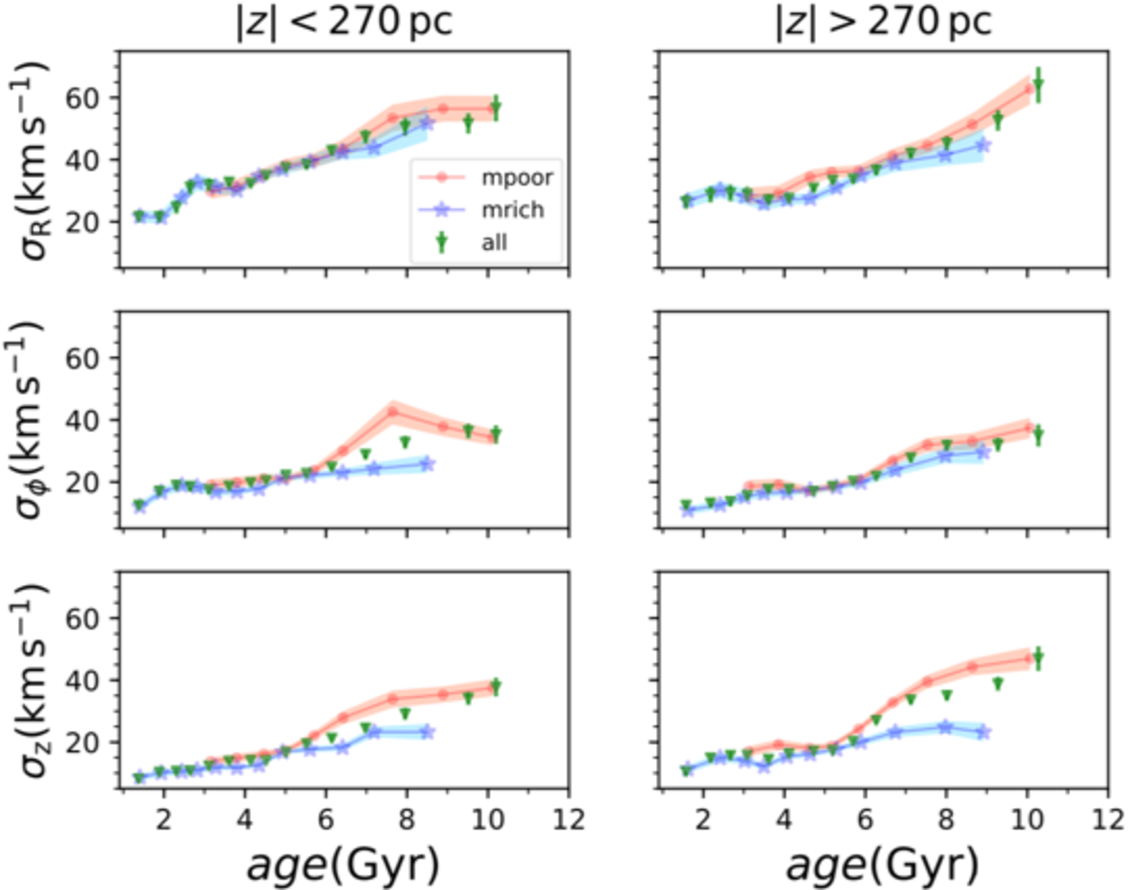
\includegraphics[width=12cm]{fig/YuLiu18_VD.pdf}
	\caption{太陽近傍星の年齢・速度分散関係\cite{YL18}。$\sigma_R、\sigma_{\phi}、\sigma_z$は円筒座標系$(R,\phi,z)$での速度分散。円盤面からの距離$|z|<270\,\mathrm{pc}$と$|z|>270\,\mathrm{pc}$とで区切っている。色の違いは金属量の違いを表しており、ピンク色は金属量が少ない (metal poor) サンプル、青色は金属量が多い (metal rich) サンプル、緑色の点は両方を合わせたサンプルの速度分散となっている。}
	\label{VDbyYL18}
\end{center}
\end{figure*}

%%%%%%%%%%%%%%%%%%%%%%%%%%%%%%%%%%%%%%%%%%%%%%%%%%%%%%%%%%%%%%%%%%%%%

大量な星のサンプルの固有運動と視線速度からオールト定数を決定するとき、それらの値を出すときの過程と潜在的な平均速度場に関する解釈の両方を含む様々な問題に直面する。

まず、若い星では運動集団や渦状腕のような非平衡な効果が平均速度$\overline{\pmb{v}}$に影響する。これは主に小さい速度分散の集団に影響する。また、サンプル数が少なすぎる場合、系統速度場の中の太陽近傍の変則的なものがオールト定数に影響する。さらに、特に古い星ではasymmetric driftの効果によって円運動の系統速度から大きく外れる。軸対称な系では、この効果はStr\"{o}mbergのasymmetric drift関係を用いて推定できる。この効果により、$A$は$3\,\mathrm{km\,s^{-1}kpc}$に満たない程度の値だけ小さくなるが、$B$はほとんど変化しない。

太陽から遠いサンプルを使用するほど、系統速度のテイラー展開の高次の項が効いてきてしまう。年周視差と速度の間に非線形の相関がある場合にこの項は特に大きく影響する。銀河系のバーのOLR (outer Lindblad resonance) が効く場所では不連続な系統場が発生し、それがオールト定数の測定を間違えさせる。年周視差の平均$\overline{\varpi}$がサンプルの銀経$l$の方向に対して依存性 (モード) を持ってしまう状態をモードミキシング (Mode mixing) という。モードミキシングがあると、固有運動は数$\mathrm{km\,s^{-1}kpc}$までの範囲でオールト定数と区別できなくなってしまう。本論文で使用する観測データのモードについては\ref{観測データ}で記述する。

%表\ref{table1}では、\cite{OD03}を参考にオールト定数を決定するときの問題点を挙げている。

% \begin{table}[htb]
% \centering
% {\small
%   \begin{tabular}{c|c|p{10cm}} \hline
%     状態 & 表記法 & 定義と説明\\ \hline
%     1 & $A,B,C,K$ & オールト定数:銀河ポテンシャル中の\colorbox{red}{閉じ}た軌道で作られる(仮定の)速度場$\pmb{v}(\pmb{r})$の発散、回転、剪断\\
%     2$^a$ & $\overline{A},\overline{B},\overline{C},\overline{K}$ & 最も得たい値:星の集団の速度場$\pmb{v}(\pmb{r})$の発散、回転、剪断\\
%     3$^b$ & $\widetilde{A},\widetilde{B},\widetilde{C},\widetilde{K}$ & 実際に得られる値:星の集団から測定される固有運動のフーリエ係数\\
%     \hline
%   \end{tabular} \label{table1}
% \vskip 3pt
% \begin{minipage}{13cm}
% \textit{$^a$}状態1と2の違いの理由として考えられるものを挙げる。(i)若い星:運動集団や渦状腕のような非平衡の効果が\colorbox{red}{閉じ}た軌道の速度場から$\pmb{\overline{v}}$を予想外な値に導く。これは主に小さい速度分散の集団に影響する。(ii)サンプルの大きさが小さすぎる場合、系統場(systematic field)の中の太陽近傍の変則的なものがオールト定数に反映される。(iii)特に古い星ではasymmetric driftの効果によって\colorbox{red}{閉じ}た軌道の系統速度から外れる。軸対称な系では、この効果はStr\"{o}mbergのasymmetric drift関係を用いて推定できる。この効果により、$A$は$3\,\mathrm{km\,s^{-1}kpc}$に満たない程度の値だけ小さくなるが、$B$はほとんど変化しない。\\
% \textit{$^b$}状態2と3の違いの理由として考えられるものを挙げる。(i)太陽から遠いサンプルを使用するほど、系統速度のテイラー展開の高次の項が効いてきてしまう。年周視差と速度の間に非線形の相関がある場合にこの項は特に大きく影響する。(ii)銀河系のバーのOLR (outer Lindblad resonance) が効く場所では不連続な系統場が発生し、それがオールト定数の測定を間違えさせる。(iii)年周視差の平均$\overline{\varpi}$がサンプルの銀経$l$の方向に対して依存性 (モード) を持ってしまう状態をモードミキシング (Mode mixing) という。モードミキシングがあると、固有運動は数$\mathrm{km\,s^{-1}kpc}$までの範囲でオールト定数と区別できなくなってしまう。
% \end{minipage}
% }
% \end{table}



%%%%%%%%%%%%%%%%%%%%%%%%%%%%%%%%%%%%%%%%%%%%%%%%%%%%%%%%%%
%%%%%%%%%%%%%%%%%%%%%%%%%%%%%%%%%%%%%%%%%%%%%%%%%%%%%%%%%%
%%%%%%%%%%%%%%%%%%%%%%%%%%%%%%%%%%%%%%%%%%%%%%%%%%%%%%%%%%


\subsection{asymmetric drift \label{sec_AD}} % 導出&物理的解釈を書く
asymmetric drift速度$\pmb{v}_{\mathrm{a}}$は、天体が銀河系円盤円軌道で回転するときの速度$\pmb{V}_{\mathrm{c}}$と系統速度$\pmb{V}$を用いて次のように表される。
\begin{align}
\begin{aligned}
    \pmb{v}_{\mathrm{a}} \equiv \pmb{V}_{\mathrm{c}} - \pmb{V}\\
\end{aligned} \label{AD}
\end{align}
ここで、$\pmb{v}_{\mathrm{a}}$はasymmetric drift速度である。この速度は、太陽近傍における系統速度$\pmb{V}$の円軌道速度$\pmb{V}_{\mathrm{c}}$からの遅れを表す。この区別を明確にするために、式(\ref{AD})のようにオールト定数を書くと、以下のように書ける。
\begin{subequations}
\begin{align}
	A &= A_{\mathrm{c}} - A_{\mathrm{a}} \\
	B &= B_{\mathrm{c}} - B_{\mathrm{a}} \\
	C &= C_{\mathrm{c}} - C_{\mathrm{a}} \\
	K &= K_{\mathrm{c}} - K_{\mathrm{a}}
\end{align}
\end{subequations}
近傍の系統運動との相対的な太陽運動はLSR (Local Standard of Rest)に対しての太陽運動とasymmetric driftとに分解される(図\ref{fig1})。LSRは局所静止基準といい、太陽の位置での系統速度$\pmb{V}(\pmb{R}_{\odot})$で動く点を静止基準とするものである。

\begin{figure*}[htbp]
\begin{center}
	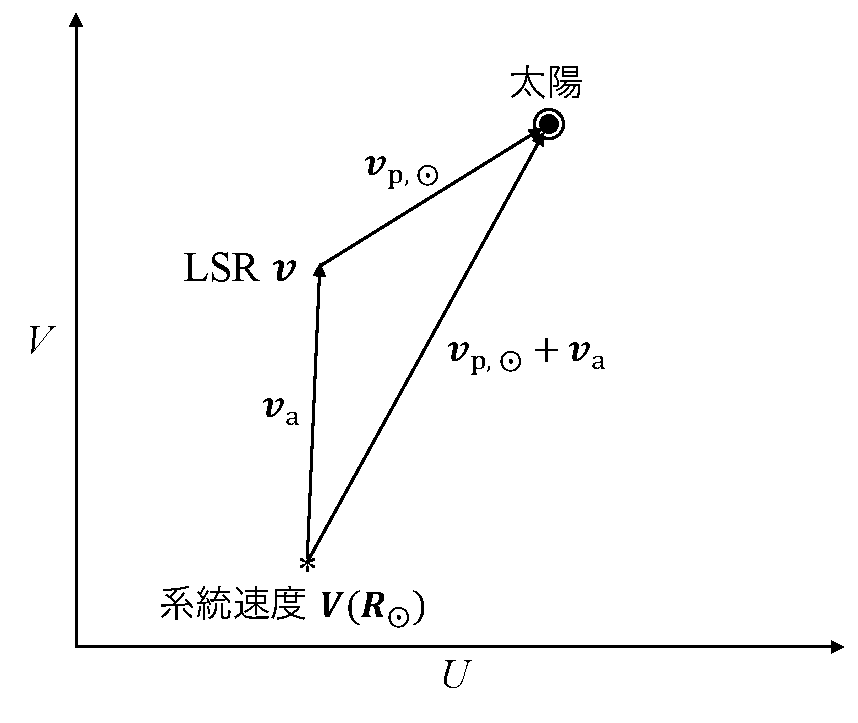
\includegraphics[width=10cm]{fig/various_velocities.pdf}
	\caption{太陽運動とasymmetric driftのスケッチ。$U、V$はそれぞれ太陽を原点として銀河中心方向、円軌道の回転方向の速度。サンプル星の系統速度$\pmb{\overline{v}}$は速度$\pmb{v}$のLSRからasymmetric drift\,$\pmb{v}_{\mathrm{a}}$の分遅れる。太陽の特異運動$\pmb{v}_{\odot}$は観測された系統速度$\pmb{V}(\pmb{R}_{\odot})$に対する太陽の速度を得るために$\pmb{v}_{\mathrm{a}}$を足す必要がある。}
	\label{fig1}
\end{center}
\end{figure*}

力学平衡状態でかつ軸対称な銀河では、$\pmb{v}_{\mathrm{a}}$のうち方位角成分$v_{\mathrm{a}}$のみが存在し、ランダムな運動 (特異運動) は系統運動に比べて非常に小さく、これはStr\"{o}mbergの関係(Jeans方程式からの導出は付録\ref{sec_JeansEq}を参照)から近似される。付録の式(\ref{Jeans_Cylindrical_pr})をここでも書く。
\begin{align}
	\frac{\partial (\nu \overline{v_R^2})}{\partial R} + \frac{\partial (\nu \overline{v_R v_z})}{\partial R} + \nu\left(\frac{\overline{v_R^2} - \overline{v_{\phi}^2}}{R} + \frac{\partial \Phi}{\partial R} \right) = 0 \label{eqJeans448}
\end{align}
この式は円筒座標系で表示されたJeans方程式において動径方向の速度$v_R$の1次モーメントを取ることで得られる (付録を参照)。$v_R、v_{\phi}、v_z$は銀河中心を静止基準とするときの星の速度であり、平均をとると$\overline{v_R}=V_R、\overline{v_{\phi}}=V_{\phi}、\overline{v_z}=V_z$のように系統速度と等しくなる。ここで、文字上部の横棒は平均を意味する。式(\ref{eqJeans448})の第2項は無視できるものとし、$\overline{v_R}=0$とすると、
\begin{align}
	\frac{\overline{v_{\phi}^2}}{R} = \frac{1}{\nu}\frac{\partial(\nu\sigma_R^2)}{\partial R} + \frac{\partial \Phi}{\partial R} \label{eqJeans452}
\end{align}
となる。速度分散が非常に小さいときには、円運動する星の速度を$v_{\mathrm{c}}$と書けば$v_{\phi}\simeq v_{\mathrm{c}}$と近似できる。そのため、$\frac{\overline{v_{\phi}^2}}{R}\simeq \frac{v_{\mathrm{c}}^2}{R} $は遠心力を表す項と考えられる。また、$\frac{\partial \Phi}{\partial R}$は明らかに中心力を表す。速度分散が非常に小さい系では、星にかかる力は中心力と遠心力とのつり合いより$\frac{v_{\mathrm{c}}^2}{R}=\frac{\partial \Phi}{\partial R}$と書ける。この式と式(\ref{eqJeans452})とを比較すると、$\frac{1}{\nu}\frac{\partial(\nu\sigma_R^2)}{\partial R}$は天の川銀河円盤内では負の値を持つことから、$\overline{v_{\phi}^2}$は$v_{\mathrm{c}}^2$に比べて$\frac{1}{\nu}\frac{\partial(\nu\sigma_R^2)}{\partial R}$の分だけ遅くなることが分かる。式(\ref{eqJeans448})を変形し、式(\ref{AD})を使用すると
\begin{align}
\begin{aligned}
    v_{\mathrm{a}} \simeq \frac{\overline{v_R^2}}{2v_{\mathrm{c}}} \left[\frac{\sigma_{\phi}^2}{\overline{v_R^2}} - 1 - \frac{\partial \ln(\nu \overline{v_R^2})}{\partial \ln R} - \frac{R}{\overline{v_R^2}}\frac{\partial \overline{v_R v_z}}{\partial z}\right] \\
    = \frac{\sigma_R^2}{2v_{\mathrm{c}}} \left[\frac{\sigma_{\phi}^2}{\sigma_R^2} - 1 - \frac{\partial \ln(\nu \sigma_R^2)}{\partial \ln R} - \frac{R}{\sigma_R^2}\frac{\partial \sigma_{Rz}^2}{\partial z}\right]
\end{aligned} \label{AD2}
\end{align}
という式が得られる。ここで、$\nu$は星密度、$\sigma_{ij}^2 \equiv \overline{(v_i-\overline{v_i})(v_j-\overline{v_j})}=\overline{v_i v_j}-\overline{v_i}\ \overline{v_j}$は速度分散テンソルを示し、ここでは広く使われるように$\sigma_{ii}^2$を$\sigma_i^2$と短く書いている。$i,j$はそれぞれ座標系の異なる向きである。式(\ref{AD2})の1行目から2行目への式変形では$\overline{v_R}=0$と仮定している。式(\ref{AD2})から、asymmetric driftは動径速度分散の関数であり、円軌道速度と速度楕円体の軸比 (図\ref{fig:ve})、動径速度分散と星密度の傾きにも依存することがわかる。

図\ref{AD_image}は$v_{\mathrm{a}}$の物理的イメージである。式(\ref{eqJeans452})の$\frac{\overline{v_{\phi}^2}}{R}$は遠心力、$\frac{1}{\nu}\frac{\partial(\nu\sigma_R^2)}{\partial R}$は速度分散勾配による圧力、$\frac{\partial \Phi}{\partial R}$は重力による中心力にあたる。$\frac{1}{\nu}\frac{\partial(\nu\sigma_R^2)}{\partial R}$が天の川銀河の内側から外側に向かって圧力勾配のように働き、銀河回転速度を遅くする。
\begin{figure*}[htbp]
\begin{center}
	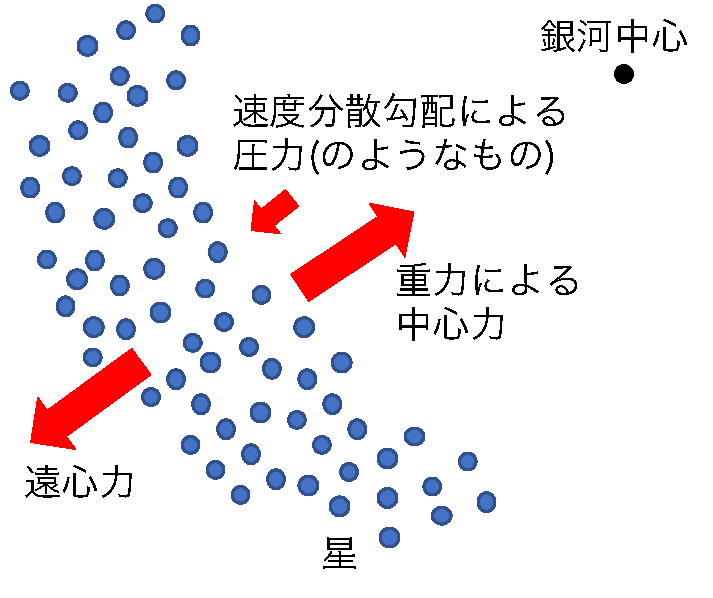
\includegraphics[width=7cm]{fig/AD_image.pdf}
	\caption{asymmetric driftの物理的イメージ。天の川銀河円盤を銀河北極方向から見下ろすような状態になっている。速度分散を持つ円盤星の中では速度分散勾配が圧力勾配のように働く。}
	\label{AD_image}
\end{center}
\end{figure*}

ここで、速度楕円体の説明をする。空間上のある$i$方向の速度分散は$\sigma_i^2 \equiv \overline{(v_i-\overline{v_i})}^2$、$i$方向と$j$方向の間の速度分散テンソルは$\sigma_{ij}^2 \equiv \overline{(v_i-\overline{v_i})(v_j-\overline{v_j})}$と定義される。このとき、$\sigma_i$を半長軸とする楕円体を定義でき、これを速度楕円体と呼ぶ。図\ref{fig:ve}は速度楕円体を2次元面に投影したときの例である。速度楕円体は一般に3軸非対称であり、半長軸の方向は座標軸とは一致するとは限らない。速度楕円体の長軸と座標軸との傾き、例えば$i$軸から$j$軸に向かって$l_{ij}$だけ傾いているとき、
\begin{align}
    \tan(2l_{ij}) = \frac{2\sigma _{ij}^2}{\sigma_i^2 \sigma_j^2}
\end{align}
と表すことができる。

\begin{figure*}[htbp]
\begin{center}
	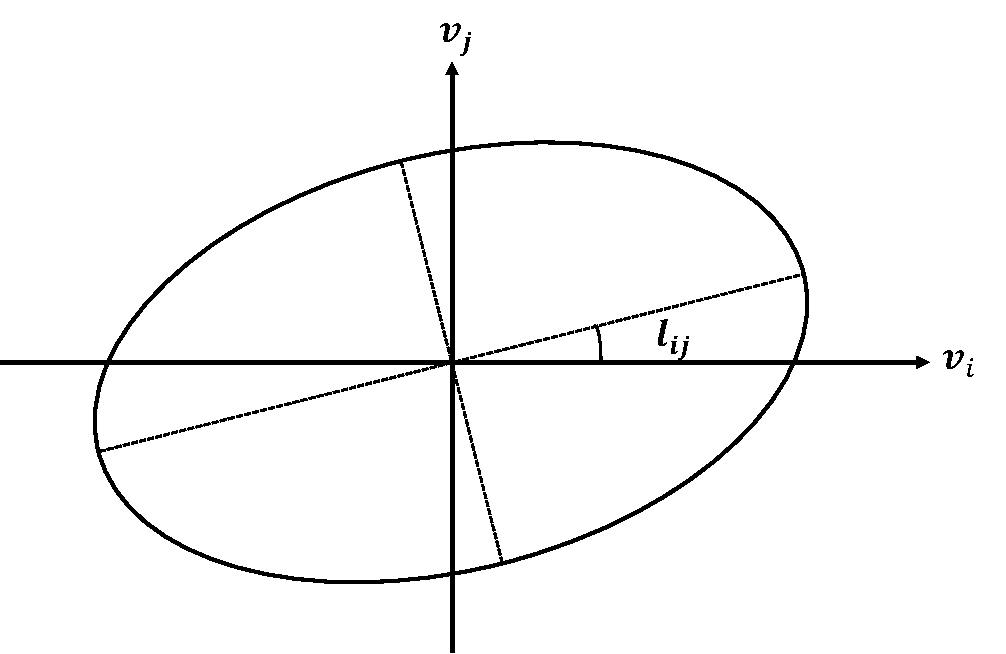
\includegraphics[width=10cm]{fig/velocity_ellipsoid.pdf}
	\caption{速度楕円体を2次元に投影したときの図。楕円は速度分散の1$\sigma$にあたる点を結んだ線である。$l_{ij}$は座標軸を図のようにとったときの楕円の主軸との傾きを表す。$\sigma_i$を長軸の長さ、$\sigma_j$を短軸の長さとすると、速度楕円体の軸比は$\frac{\sigma_i}{\sigma_j}$と書ける。}
	\label{fig:ve}
\end{center}
\end{figure*}

式(\ref{AD2})について、\cite{BT2008}の近似にしたがって式変形をしてみる。$\sigma_{\phi}^2/\sigma_R^2 = 0.35$とする。$\nu、\sigma_R^2 \propto e^{-R/h_R}、R/h_R = 3.2$とするとき、
$\frac{\sigma_{\phi}^2}{\sigma_R^2} - 1 - \frac{\partial \ln{(\nu \sigma_R)}}{\partial \ln{R}} = 0.35 - 1 + 6.4 = 5.75$となる。式(\ref{AD2})の右辺最終項について、\cite{BT2008}では次の2つの場合について書かれている。
(i)速度楕円体の主軸が$(R,\phi,z)$の座標軸に沿っているときには$\frac{\partial(\overline{v_R v_z})}{\partial z} = 0$となる。
(ii)速度楕円体の主軸が銀河中心を中心とした球対称座標系$(r,\theta,\phi)$に沿っているとき、$\overline{v_R v_z} \simeq (\sigma_R^2 - \sigma_{\sigma}^2)\frac{z}{R}$から$\frac{R}{\sigma_R^2} \frac{\partial (\overline{v_R v_z})}{\partial z} \simeq 0.8$となる。$\frac{\partial(\overline{v_R v_z})}{\partial z}$は(i)、(ii)の中間的な値であるとすると、式(\ref{AD2})の角括弧内は$5.4 \pm 0.4$と計算できる。さらに回転速度$v_{\phi} = \SI{200}{km.s^{-1}}$とすると、$v_{\mathrm{a}} \simeq \frac{\sigma_R^2}{82 \pm 6\,\si{km.s^{-1}}}\,\si{km.s^{-1}}$となる。この式をさらにシンプルに表現すると
\begin{align}
\begin{aligned}
    v_{\mathrm{a}} \simeq \frac{\sigma_R^2}{80}\,\si{km.s^{-1}}
\end{aligned} \label{AD3}
\end{align}
となる (\cite{BT2008})。



%%%%%%%%%%%%%%%%%%%%%%%%%%%%%%%%%%%%%%%%%%%%%%%%%%%%%%%%%%%%%%%%%%%%%%%%%%%%%%%%%%%%%%%%
%%%%%%%%%%%%%%%%%%%%%%%%%%%%%%%%%%%%%%%%%%%%%%%%%%%%%%%%%%%%%%%%%%%%%%%%%%%%%%%%%%%%%%%%

\subsection{asymmetric driftのオールト定数への影響}
$A,B,C,K$は系統速度に対して速度分散が非常に小さいような系での軌道の系統場から出され、ポテンシャルに従った項で直接的に解釈される一方、$\overline{A},\overline{B},\overline{C},\overline{K}$は実際の星の集団の系統場を表す。$\overline{A},\overline{B},\overline{C},\overline{K}$は式(\ref{eq2})あるいは(\ref{eq2.5a})-(\ref{eq2.5d})において$\pmb{v}$を$\pmb{\overline{v}}$で置き換えたもので、$A_{\mathrm{a}},B_{\mathrm{a}},C_{\mathrm{a}},K_{\mathrm{a}}$は同じく$\pmb{v}$を$\pmb{v}_{\mathrm{a}}$で置き換えたものである。

ここで、式(\ref{AD2})について、$\nu,\sigma_{ij}$がそれぞれスケール長$h_R,h_{\sigma}$で指数関数的に変化すると仮定し、$\nu \propto e^{
-R/h_R}、\sigma_{ij}^2 \propto e^{-R/h_{\sigma}}、hv_{\mathrm{a}} \simeq \sigma_{R}^2$という仮定を用いる。また、右辺第3項は$-\partial\,\mathrm{ln}(\nu \sigma_R^2)/\partial\,\mathrm{ln} R = R(1/h_R + 1/h_{\sigma})$と変形できる。さらに右辺第4項は無視できるから、
\begin{align}
\begin{aligned}
    2V_{\phi}v_{\mathrm{a}} \simeq \sigma_R^2 \left[\frac{\sigma_{\phi}^2}{\sigma_R^2} - 1 + R\left(\frac{1}{h_R} + \frac{2}{h_{\sigma}}\right)\right]
\end{aligned} \label{AD5}
\end{align}
となる。ここで、$\sigma_{ij} \propto e^{-R/h_{\sigma}}$から、$D$を定数として$\sigma_{\phi}^2/\sigma_R^2 - 1 = D$と書けるから、
\begin{align}
\begin{aligned}
    2V_{\phi}v_{\mathrm{a}} \simeq \sigma_R^2 \left[D + R\left(\frac{1}{h_R} + \frac{2}{h_{\sigma}}\right)\right]
\end{aligned} \label{AD6}
\end{align}
式 (\ref{AD6})の両辺のlogをとり$R$で微分すると、
\begin{align}
\begin{aligned}
    \ln2+\ln V_{\phi}+\ln v_{\mathrm{a}} &\simeq \ln \sigma_R^2 +\ln \left[D + R\left(\frac{1}{h_R} + \frac{2}{h_{\sigma}}\right)\right] \\
    \frac{\partial \ln V_{\phi}}{\partial R}+\frac{\partial \ln v_{\mathrm{a}}}{\partial R} &\simeq -\frac{2}{h_{\sigma}} + \frac{1/h_R + 1/h_{\sigma}}{D +R\left(1/h_R + 1/h_{\sigma}\right)} \\
\end{aligned} \label{AD8}
\end{align}
したがって、式(\ref{AD6}),(\ref{AD8})と$hv_{\mathrm{a}} \simeq \sigma_R^2$から
\begin{align}
\begin{aligned}
    \frac{\partial \mathrm{ln}v_{\mathrm{a}}}{\partial R} \simeq -\frac{2}{h_{\sigma}} + \frac{h}{2V_{\phi}}\left(\frac{1}{h_R} + \frac{2}{h_{\sigma}}\right) - \frac{\partial \mathrm{ln}V_{\phi}}{\partial R}
\end{aligned} \label{AD9}
\end{align}
となる。

asymmetric driftは軸対称を仮定していることから、式(\ref{ABsym}),(\ref{AD9})を利用して$A_{\mathrm{a}},B_{\mathrm{a}}$は次のように表すことができる。
\begin{subequations}
\begin{align}
	A_{\mathrm{a}} &=\frac{1}{2}\left( \frac{v_{\mathrm{a}}}{R} - \frac{\partial v_{\mathrm{a}}}{\partial R} \right)_{R=R_{\odot}} = \frac{v_{\mathrm{a}}}{2}\left[\frac{1}{R_{\odot}} + \frac{2}{h_{\sigma}} - \frac{h}{2V_{\phi}}\left(\frac{1}{h_R} + \frac{2}{h_{\sigma}}\right)\right] \\
	B_{\mathrm{a}} &=\frac{1}{2}\left( -\frac{v_{\mathrm{a}}}{R} - \frac{\partial v_{\mathrm{a}}}{\partial R} \right)_{R=R_{\odot}} = \frac{v_{\mathrm{a}}}{2}\left[-\frac{1}{R_{\odot}} + \frac{2}{h_{\sigma}} - \frac{h}{2V_{\phi}}\left(\frac{1}{h_R} + \frac{2}{h_{\sigma}}\right)\right]
\end{align} \label{ABaxisym}
\end{subequations}
$R_{\odot}=8.2\,\mathrm{km\,s^{-1}},h_R =2.68\,\mathrm{kpc}, h_{\sigma}=9\,\mathrm{kpc}$ (\cite{Piffl14}),$V_{\phi}=236\,\mathrm{km\,s^{-1}}$ (\cite{Kawata2019}) とするとき
$A_{\mathrm{a}}\approx0.122v_{\mathrm{a}}, B_{\mathrm{a}}\approx0.003v_{\mathrm{a}}$となり、$h_R,R_{\odot},V_{\phi}$とはほぼ独立している。すなわち、$B$はasymmetric driftの影響をほとんど受けないが、$A_{\mathrm{a}}$は$v_{\mathrm{a}}=20\,\si{km.s^{-1}}$のときには2.4程度の大きさとなり、asymmetric driftの影響を少し受ける。

%%%%%%%%%%%%%%%%%%%%%%%%%%%%%%%%%%%%%%%%%%%%%%%%%%%%%%%%%%%%%%%%%%%%%%%%%%%%%%%%%%%%%%%%
%%%%%%%%%%%%%%%%%%%%%%%%%%%%%%%%%%%%%%%%%%%%%%%%%%%%%%%%%%%%%%%%%%%%%%%%%%%%%%%%%%%%%%%%

\subsection{asymmetric driftを考慮した観測方程式 \label{sec_ObsAD}}
ここで、観測方程式にasymmetric drift項を追加することを考える。円筒座標系で$(0,v_a,0)$とする。また、$\bf{P、Q}$はそれぞれ$(v_x,v_y,v_z) \to (v_l,v_ b,v_{\mathrm{los}})、(v_{R},v_{\phi},v_z) \to (v_x,v_ y,v_z)$のようにベクトルを変換する行列であるとする。このとき$\bf{P,Q}$は
\begin{align}
\begin{aligned}
	\bf{P}=
	\left(
	\begin{array}{ccc}
	 	-\sin{l} & -\cos{l}\sin{b} & \cos{l}\cos{b}\\
		 \cos{l} &  \sin{l}\cos{b} & \sin{l}\cos{b}\\
		0 & \cos{b} & \sin{b}
	\end{array}
	\right)
\end{aligned}
\end{align}
\begin{align}
\begin{aligned}
	\bf{Q}=
	\left(
	\begin{array}{ccc}
	 	\cos{\phi} & -\sin{\phi} & 0\\
		\sin{\phi} &  \cos{\phi} & 0\\
		0 & 0 & 1
	\end{array}
	\right)
\end{aligned} \label{Q}
\end{align}
銀河座標系でのasymmetric drift項を$(v_{\mathrm{a},l},v_{\mathrm{a},b},v_{\mathrm{a,los}})$と書くと、
\begin{align}
\begin{aligned}
	\left(
	\begin{array}{c}
	 	v_{\mathrm{a},l}\\
		v_{\mathrm{a},b}\\
		v_{\mathrm{a,los}}
	\end{array}
	\right)
	=& \bf{P} \bf{Q}
	\left(
	\begin{array}{c}
	 	0\\
		v_a\\
		0
	\end{array}
	\right)
\end{aligned}
\end{align}
となる。式(\ref{ObsEq})にasymmetric drift項を追加した式は
\begin{subequations}
\begin{align}
	\mu^{*,\mathrm{AD}}_l(l_i,b_i,\varpi_i) &= (A\cos2l_i - C\sin2l_i + B)\cos b_i + \varpi_i(U_{\odot}\sin l_i - V_{\odot}\cos l_i) - \varpi_i v_{\mathrm{a},l} \\
	\mu^{\mathrm{AD}}_b(l_i,b_i,\varpi_i) &= -(A\sin2l_i + C\cos2l_i + K)\sin b_i \cos b_i \nonumber \\
	                          & \hspace{2cm} + \varpi_i[(U_{\odot}\cos l_i + V_{\odot} \sin l_i)\sin b_i - W_{\odot} \cos b_i] - \varpi_i v_{\mathrm{a},b} \\
	v^{\mathrm{AD}}_{\mathrm{los}}(l_i,b_i,\varpi_i) &= (K + C\cos2l_i + A\sin2l_i)\varpi_i^{-1} cos^2 b_i \nonumber \\
	                      & \hspace{2cm} - [(U_{\odot}\cos l_i + V_{\odot} \sin l_i)\cos b_i + W_{\odot} \sin b_i] - v_{\mathrm{a,los}}
\end{align} \label{ObsEqAD}
\end{subequations}
となる。添字のADは、asymmetric driftを考慮したモデルの式であることを示している。



%%%%%%%%%%%%%%%%%%%%%%%%%%%%%%%%%%%%%%%%%%%%%%%%%%%%%%%%%%%%%%%%%%%%%%%%
%%%%%%%%%%%%%%%%%%%%%%%%%%%%%%%%%%%%%%%%%%%%%%%%%%%%%%%%%%%%%%%%%%%%%%%%
%%%%%%%%%%%%%%%%%%%%%%%%%%%%%%%%%%%%%%%%%%%%%%%%%%%%%%%%%%%%%%%%%%%%%%%%



% \section{Asymmetric drift \label{Asymmetric drift}}
% この節では\cite{BT2008}にしたがってasymmetric driftについて説明する。

% 重力ポテンシャルが$\Phi$のとき$H=\frac{1}{2}v^2 + \Phi(\pmb{x},t)$で書けるような直交座標系での無衝突ボルツマン方程式は次のようになる。
% \begin{align}
% 	\frac{\partial f}{\partial t} + p_R\frac{\partial f}{\partial R} + \frac{p_{\phi}}{R^2}\frac{\partial f}{\partial \phi} + p_z\frac{\partial f}{\partial z} - \left(\frac{\partial \Phi}{\partial R} - \frac{p_{\phi}^2}{R^3} \right)\frac{\partial f}{\partial p_R} - \frac{\partial \Phi}{\partial \phi}\frac{\partial f}{\partial p_{\phi}} - \frac{\partial \Phi}{\partial z}\frac{\partial f}{\partial p_z} = 0
% \end{align}
% 円筒座標系では$H = \frac{1}{2}(p_R^2 + p_{\phi}^2/R^2 + p_z^2) + \Phi$となり、そのため
% \begin{align}
% 	\frac{\partial f}{\partial t} + \frac{\partial f}{\partial \pmb{q}} \frac{\partial H}{\partial \pmb{p}} - \frac{\partial f}{\partial \pmb{p}} \frac{\partial H}{\partial \pmb{q}} = 0
% \end{align}
% から
% \begin{align}
% 	\frac{\partial f}{\partial t} + p_R\frac{\partial f}{\partial R} + \frac{p_{\phi}}{R^2}\frac{\partial f}{\partial \phi} + p_z\frac{\partial f}{\partial z} - \left(\frac{\partial \Phi}{\partial R} - \frac{p_{\phi}^2}{R^3} \right)\frac{\partial f}{\partial p_R} - \frac{\partial \Phi}{\partial \phi}\frac{\partial f}{\partial p_{\phi}} - \frac{\partial \Phi}{\partial z}\frac{\partial f}{\partial p_z} = 0   \label{eq193}
% \end{align}
% のようになる。考えている系が定常状態で軸対称であると仮定すると、$t$と$\phi$に関する微分の項は全て消える。これらの仮定から、式(\ref{eq193})は
% \begin{align}
% 	p_r\frac{\partial f}{\partial R} + p_z\frac{\partial f}{\partial z} - \left(\frac{\partial \Phi}{\partial R} - \frac{p_{\phi}^2}{R^3} \right)\frac{\partial f}{\partial p_R} - \frac{\partial \Phi}{\partial z}\frac{\partial f}{\partial p_z} = 0    \label{eq196}
% \end{align}
% と簡単に書ける。この式に$p_R$をかけて全運動量で積分し、式(\ref{eq196})を用いて
% \begin{align}
% 	\frac{\partial (\nu \overline{v_{\mathrm{los}}^2})}{\partial R} + \frac{\partial (\nu \overline{v_{\mathrm{los}} V_z})}{\partial R} + \nu\left(\frac{\overline{v_{\mathrm{los}}^2} - \overline{V_{\phi}^2}}{R} + \frac{\partial \Phi}{\partial R} \right) = 0   \label{eq200}
% \end{align}
% となる。ここで、asymmetric drift速度
% \begin{align}
% 	v_{\mathrm a} \equiv v_{\mathrm c} - \overline{V_{\phi}}
% \end{align}
% を考える。$v_{\mathrm c}$は太陽近傍での円軌道速度である。

% 今、円盤は定常状態でその赤道面に対して対称であると考える。また、太陽は銀河赤道の近くに位置しているため、$z=0$での式(\ref{eq200})を考えればよい。対称性より$\partial \nu/\partial z = 0$であるから、次の式を得る。
% \begin{align}
% 	\frac{R}{\nu}\frac{\partial(\nu \overline{v_{\mathrm{los}}^2})}{\partial R} + R\frac{\partial(\overline{v_{\mathrm{los}} V_z})}{\partial z} + \overline{v_{\mathrm{los}}^2} - \overline{V_{\phi}^2} + R\frac{\partial \Phi}{\partial R} = 0
% \end{align}
% $\sigma_{ij}^2 = \overline{v_i v_j} - \overline{v_i}\overline{v_j}$とasymmetric driftの定義から、
% \begin{align}
% 	\sigma_{\phi}^2 - \overline{v_{\mathrm{los}}^2} &-\frac{R}{\nu}\frac{\partial(\nu \overline{v_{\mathrm{los}}^2})}{\partial R} - R\frac{\partial(\overline{v_{\mathrm{los}} V_z})}{\partial z} = v_{\mathrm c}^2 - \overline{V_{\phi}^2} \\
% 	&= (v_{\mathrm c} - \overline{V_{\phi}}) (v_{\mathrm c} + \overline{V_{\phi}}) = v_{\mathrm a}(2v_{\mathrm c} - v_{\mathrm a})
% \end{align}
% となる。$2v_{\mathrm c}$に比べて$v_{\mathrm a}$が無視できるとき、Str\"{o}mbergのasymmetric drift方程式
% \begin{align}
% 	v_{\mathrm a} \simeq \frac{\overline{v_{\mathrm{los}}^2}}{2v_{\mathrm c}}\left[\frac{\sigma_{\phi}^2}{\overline{v_{\mathrm{los}}^2}} - 1 - \frac{\partial\ln(\nu\overline{v_{\mathrm{los}}^2})}{\partial\ln R} - \frac{R}{\overline{v_{\mathrm{los}}^2}}\frac{\partial(\overline{v_{\mathrm{los}} V_z})}{\partial z}\right]   \label{eq221}
% \end{align}
% が得られる。

% \cite{BM1998}の表10.2から、$\sigma_{\phi}^2/\overline{v_{\mathrm{los}}^2}=0.35$という値を使用することにする。$\nu,\overline{v_{\mathrm{los}}^2}$はともに$e^{-R/R_{\mathrm d}}$に比例し、$R/R_{\mathrm d}=3.2$と仮定する。以上の仮定を用いると、式(\ref{eq221})の角括弧内の前の3項の合計は5.8となる。最後の項は銀河系円盤面のちょうど上の点での速度楕円体の向きに依存するため、測定することが難しい。これについては次の2つの極限での可能性がある。座標系の中心は銀河中心とし、(1)楕円体の主軸が円筒座標系$(R,\phi,z)$の座標軸に沿った向き、(2)主軸が球対称座標系$(R,\theta,\phi)$の座標軸に沿った向きになる場合に2つの可能性である。軌道積分(\cite{BS1983})は、実際にはこの2つの可能性のほぼ真ん中の状態になっていると示唆している。(1)の場合では$\overline{v_{\mathrm{los}} V_z}$はzに関して独立であり、(2)に場合では$\overline{v_{\mathrm{los}} V_z}\simeq (\overline{v_{\mathrm{los}}^2}-\overline{V_z^2})(z/R)$と書け、この項は$-(1-\overline{V_z^2}/\overline{v_{\mathrm{los}}^2})\simeq -0.8$となる。これらの値の平均をとると、角括弧内の値は$5.4\pm 0.4$となり、そのため$v_{\mathrm a}\simeq \overline{v_{\mathrm{los}}^2}/(81.5 \pm 6\,\mathrm{km\,s^{-1}})$となる。


% 本研究ではまず$\overline{v_{\mathrm{los}}}=0\,\mathrm{km\,s^{-1}}$と仮定し、$\sigma_{v_{\mathrm{los}}}^2 = \overline{v_{\mathrm{los}}^2}$とする。さらに、$\nu \propto e^{-R/h_R}, \sigma_{vR} \propto e^{-R/h_{\sigma}}$と仮定する。ここで、$h_R,h_{\sigma}$はそれぞれ星の密度分布のスケール長、速度分散のスケール長である。\cite{Bovy2012b}では$h_R=3\,\mathrm{kpc},h_{\sigma}=8\,\mathrm{kpc}$、\cite{Kawata2019}では$h_R=20\,\mathrm{kpc},h_{\sigma}=20\,\mathrm{kpc}$が使用されていたが、\cite{BH2016}の表5から本研究では$h_R=2.5\,\mathrm{kpc},h_{\sigma}=8\,\mathrm{kpc}$を採用する。また、式(\ref{eq221})の角括弧内の最後の項は\cite{BT2008}と同様の値を採用する。これらのことから、asymmetric driftは
% \begin{align}
% 	v_{\mathrm a} &\simeq \frac{\sigma_{R}^2}{2v_{\mathrm c}}\left[\frac{\sigma_{\phi}^2}{\sigma_{R}^2} - 1 - \frac{\partial\ln(\nu\sigma_{R}^2)}{\partial\ln R} - \frac{R}{\overline{v_{\mathrm{los}}^2}}\frac{\partial(\overline{v_{\mathrm{los}} V_z})}{\partial z}\right]\\
% 	&= \simeq \frac{\sigma_{R}^2}{2v_{\mathrm c}}\left[\frac{\sigma_{\phi}^2}{\sigma_{R}^2} + R\left(\frac{1}{h_R}+\frac{2}{h_{\sigma}}\right) - 1.4\right]
% \end{align} \label{AD244}
% となる。


% %%%%%%%%%%%%%%%%%%%%%%%%%%%%%%%%%%%%%%%%%%%%%%%%%%%%%%%%%%%%%%%%%%%%%%%%%%%%%%%%%%%%%%%%%%%%%%%%
% %%%%%%%%%%%%%%%%%%%%%%%%%%%%%%%%%%%%%%%%%%%%%%%%%%%%%%%%%%%%%%%%%%%%%%%%%%%%%%%%%%%%%%%%%%%%%%%%
% %%%%%%%%%%%%%%%%%%%%%%%%%%%%%%%%%%%%%%%%%%%%%%%%%%%%%%%%%%%%%%%%%%%%%%%%%%%%%%%%%%%%%%%%%%%%%%%%

% \section{速度楕円体}
% 空間上のある$i$方向の速度分散は$\sigma_i^2 \equiv \overline{(v_i-\overline{v_i})}^2$、$i$方向と$j$方向の間の速度分散テンソルは$\sigma_{ij}^2 \equiv \overline{(v_i-\overline{v_i})(v_j-\overline{v_j})}$と定義される。このとき、$\sigma_i$を半長軸とする楕円体を定義でき、これを速度楕円体と呼ぶ。速度楕円体は一般に3軸非対称であり、半長軸の方向は座標軸とは一致するとは限らない。速度楕円体の長軸と座標軸との傾き、例えば$i$軸から$j$軸に向かって$l_{ij}$だけ傾いているとき、
% \begin{align}
%     \tan(2l_{ij}) = \frac{2\sigma _{ij}^2}{\sigma_i^2 \sigma_j^2}
% \end{align}
% と表すことができる。

% \begin{figure*}[htbp]
% 	\centering
% 	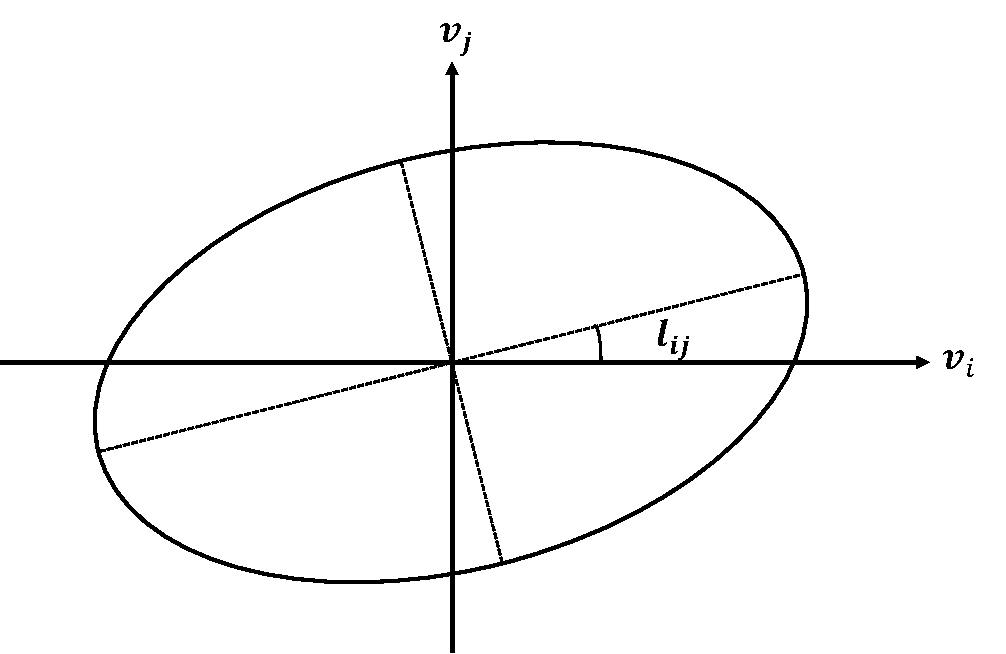
\includegraphics[width=13cm]{fig/velocity_ellipsoid.pdf}
% 	\caption{速度楕円体を2次元に投影したときの図。楕円は速度分散の1$\sigma$にあたる点を結んだ線である。$l_{ij}$は座標軸を図のようにとったときの楕円の主軸との傾きを表す。}
% 	\label{fig:ve}
% \end{figure*}
\chapter{模擬データによる定量評価}
% 3.1 模擬データの生成方法
% 3.2 解析方法
%  3.2.1 ベイズ推定の基礎
%  3.2.2 解析に用いる尤度関数
% 3.3 模擬データを用いた定量評価の結果
%  3.3.1 asymmetric driftの影響 (今、メールでは名称を省略しています)
%  3.3.2 ...影響
%  3.3.7 ...影響
% 3.4 解析結果のまとめ


Gaiaの模擬データを生成し、それを解析することで、Asymmetri drift、視線速度の有無、速度楕円体の傾き、太陽からの距離$D$、円盤面からの距離$|z|$、データ数のそれぞれの解析への影響を定量的に評価した。この章ではそれらの結果についてまとめる。
\section{模擬データの生成方法}
観測方程式(\ref{ObsEq})に従う速度場を仮定し、密度分布には指数関数的密度分布$\rho(R,z) = \rho_0 e^{-R/R_d} e^{-z/z_d},R_d=3 \mathrm{kpc},z_d=300 \mathrm{pc}$(\cite{BH2016})を仮定している。ここで、$R,z$はそれぞれ円筒座標系での動径方向と鉛直方向の位置、$R_d,z_d$は$R,z$方向の密度分布のスケール長を示す。サンプル数は基本的に1000とし、太陽からの距離$D<1\,\mathrm{kpc}$としている。このときの3次元分布と1次元の頻度分布太陽の銀河中心からの距離は$R_0 = 8.2\ \mathrm{kpc}$(\cite{BH2016})としている。また、asymmetric driftは速度分散の銀河回転方向成分を用いて$v_{\mathrm{a}} = \sigma_R^2$として計算している。

%\subsection{模擬データの生成コード}
%以下に模擬データの作成コードのうちの1つを記述する。このコードではexponential diskを仮定し、太陽からの距離1kpc以内に1000個の星があるとしている。OLCODモデルに従った速度場を持たせている。
%\lstinputlisting[language=Python]{code/MockGenerate.py}

\begin{figure*}[htbp]
\begin{center}
	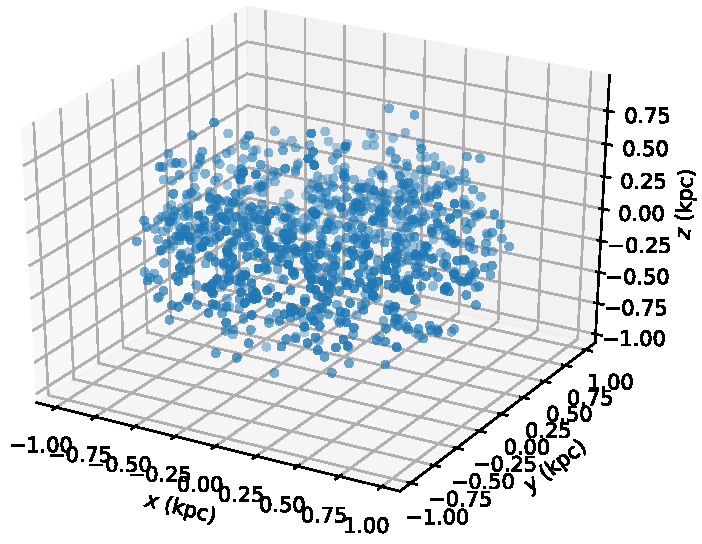
\includegraphics[width=9cm]{fig/3dMockData.pdf}
	\caption{1000個の星の模擬データの3次元分布} \label{dist3dMockData}
\end{center}
\end{figure*}

\begin{figure*}
   \centering
\begin{tabular}{ccc}
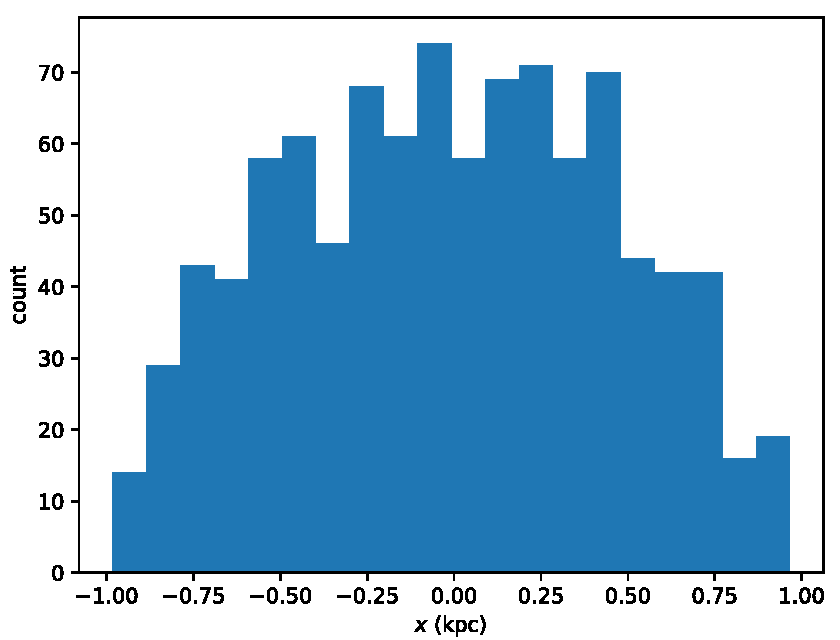
\includegraphics[width=4.5cm]{fig/dist_x.pdf}&
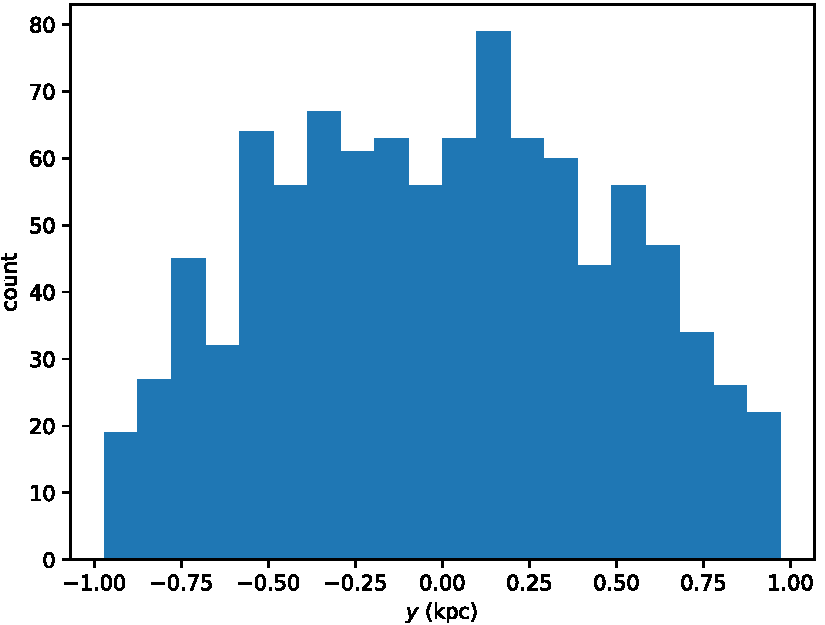
\includegraphics[width=4.5cm]{fig/dist_y.pdf}&
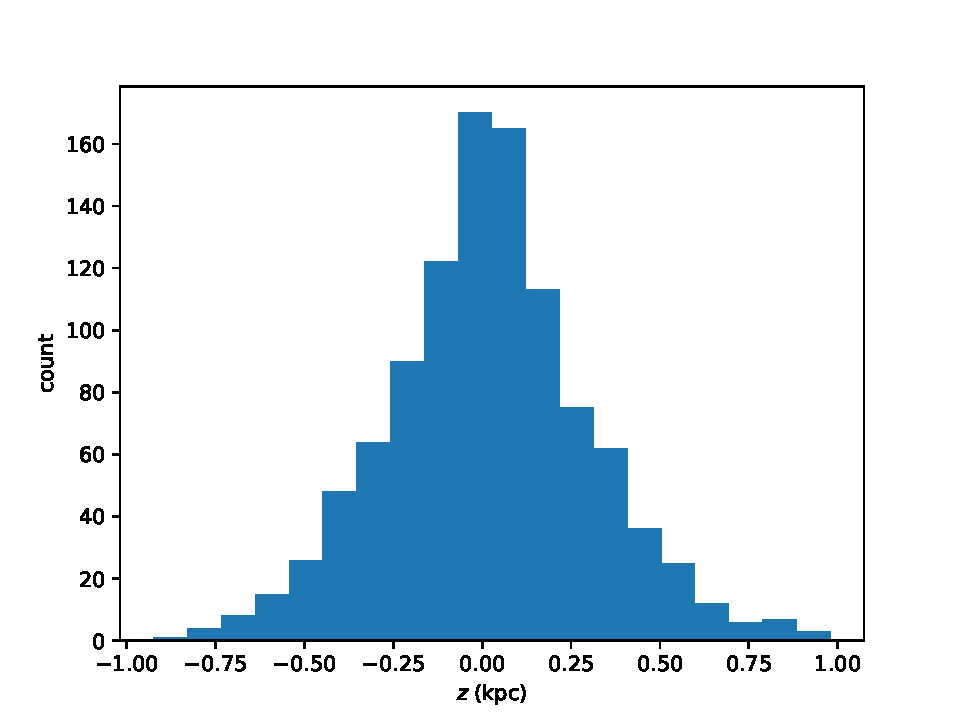
\includegraphics[width=4.5cm]{fig/dist_z.pdf}
\end{tabular}
    \caption{1000個の星の模擬データの1次元頻度分布}
    \label{distMockData}
\end{figure*}

\begin{table}
\begin{center}
%\scalebox{0.5}
%\scriptsize
%\footnotesize
%\small
\begin{tabular}{c|c|c|c} \hline
 \rowcolor{LightCyan}
 星の年齢 $\tau\ \mathrm{(Gyr)}$ & $\sigma_R\ \mathrm{(km\ s^{-1})}$ & $\sigma_{\phi}\ \mathrm{(km\ s^{-1})}$ & $\sigma_{z}\ \mathrm{(km\ s^{-1})}$\\
 \hline
 1.4 & 21.7 & 12.0 & 8.6\\
 \hline
 1.9 & 21.4 & 16.7 & 10.1\\
 \hline
 2.4 & 27.8 & 18.9 & 10.5\\
 \hline
 2.8 & 32.7 & 18.4 & 11.0\\
 \hline
 3.3 & 31.3 & 16.8 & 11.9\\
 \hline
 3.8 & 30.1 & 16.9 & 11.7\\
 \hline
 4.3 & 34.7 & 17.8 & 12.6\\
 \hline
 4.9 & 36.8 & 21.2 & 16.8\\
 \hline
 5.6 & 39.3 & 22.1 & 17.7\\
 \hline
 6.4 & 42.5 & 23.0 & 18.3\\
 \hline
 7.2 & 43.8 & 24.2 & 23.3\\
 \hline
 8.5 & 51.8 & 25.8 & 23.3\\
 \hline
\end{tabular} \label{VelocityDispersion}
\vspace{3mm}
\caption{模擬データ生成で用いた年齢と速度分散の対応表\cite{YL18}。}
\end{center}
\end{table}

%%%%%%%%%%%%%%%%%%%%%%%%%%%%%%%%%%%%%%%%%%%%%%%%%%%%%%%%%%%%%%%%%%%%%%%%%%%%%%%%
%%%%%%%%%%%%%%%%%%%%%%%%%%%%%%%%%%%%%%%%%%%%%%%%%%%%%%%%%%%%%%%%%%%%%%%%%%%%%%%%
%%%%%%%%%%%%%%%%%%%%%%%%%%%%%%%%%%%%%%%%%%%%%%%%%%%%%%%%%%%%%%%%%%%%%%%%%%%%%%%%

\section{模擬データの解析結果}
模擬データの解析では7つのパターンで模擬データ生成や解析方法を変更してオールト解析における7つの効果を調べた。表\ref{table4}、\ref{table5}はそれぞれの解析で用いた模擬データの設定と仮定を示している。asymmetric driftについては解析に際して入れる必要がある場合のみ模擬データに入れている。また、太陽は円盤面上に位置していると仮定している。

\begin{table}
\begin{center}
%\scalebox{0.5}
%\scriptsize
%\footnotesize
%\small
\begin{tabular}{l|c} \hline
 \rowcolor{LightCyan}
 パラメータ & 値\\
 \hline
 $A$ & 18 $\mathrm{km\,s^{-1} kpc^{-1}}$\\
 \hline
 $B$ & -11 $\mathrm{km\,s^{-1} kpc^{-1}}$\\
 \hline
 $C$ & -2 $\mathrm{km\,s^{-1} kpc^{-1}}$\\
 \hline
 $K$ & -1 $\mathrm{km\,s^{-1} kpc^{-1}}$\\
 \hline
 $U_{\odot}$ & 9 $\mathrm{km\,s^{-1}}$\\
 \hline
 $V_{\odot}$ & 11 $\mathrm{km\,s^{-1}}$\\
 \hline
 $W_{\odot}$ & 7.5 $\mathrm{km\,s^{-1}}$\\
 \hline
 $R_0$ & 8.2 $\mathrm{kpc}$\\
 \hline
\end{tabular}
\vspace{3mm}
\caption{模擬データ生成で用いた各パラメータの設定値。}
\label{table4}
\end{center}
\end{table}



\begin{table}
\begin{center}
%\scalebox{0.5}
%\scriptsize
%\footnotesize
%\small
\begin{tabular}{l|c|c} \hline
 \rowcolor{LightCyan}
 解析名 & asymmetric drift & 試行回数 \\
 \hline
 解析1: Asymmetric driftの解析結果への影響 & 有 & 3\\
 \hline
 解析2: 視線速度の有無による解析結果への影響 & 無 & 10\\
 \hline
 解析3: 速度楕円体の傾きの解析結果への影響 & 無 & 10\\
 \hline
 解析4: 太陽からの距離の解析結果への影響 & 無 & 10\\
 \hline
 解析5: 円盤面からの距離の解析結果への影響 & 無 & 10\\
 \hline
 解析6: サンプル数の解析結果への影響 & 無 & 10\\
 \hline
 解析7: $R_0$の値の解析結果への影響 & 有 & 3\\
 \hline
\end{tabular}
\vspace{3mm}
\caption{それぞれの解析で用いた設定。asymmetric driftの有無は、模擬データにasymmetric driftを入れたか入れないかを示している。試行回数は、模擬データを同じ設定値で生成し解析したパターン数。これは、ランダム性を可能な限り解消するためにいくつかのパターンで同じ解析を行って、全パターンの平均値を解析結果として用いている。}
\label{table5}
\end{center}
\end{table}

%%%%%%%%%%%%%%%%%%%%%%%%%%%%%%%%%%%%%%%%%%%%%%%%%%%%%%%%%%%%%%%%%%%%%%%%%%%%%%%%%%%%%%%%%%%%%%%%
%%%%%%%%%%%%%%%%%%%%%%%%%%%%%%%%%%%%%%%%%%%%%%%%%%%%%%%%%%%%%%%%%%%%%%%%%%%%%%%%%%%%%%%%%%%%%%%%
%%%%%%%%%%%%%%%%%%%%%%%%%%%%%%%%%%%%%%%%%%%%%%%%%%%%%%%%%%%%%%%%%%%%%%%%%%%%%%%%%%%%%%%%%%%%%%%%

\subsection{解析1: Asymmetric driftの解析結果への影響}
asymmetric driftの効果を入れた模擬データについて、asymmetric driftを考慮しない解析(観測方程式(\ref{ObsEq}))とasymmetric driftを考慮した解析(観測方程式(\ref{ObsEqAD}))との2通りの解析を行う。図(\ref{fig:Mock_AD})はその解析結果である。assyemtric drift無しと有りでは、$A,B,V_{\odot}$で明らかな違いがある。特に$V_{\odot}$ではasymmetric drift有りの解析結果の設定値との差が顕著であり、相対誤差

\begin{figure*}[htbp]
	\centering
	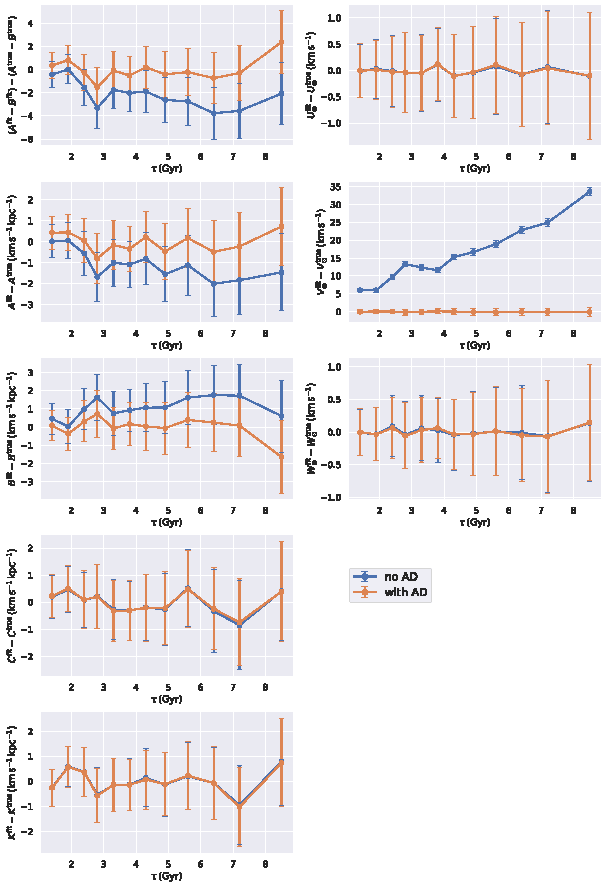
\includegraphics[width=15cm]{fig/Mock_AD.pdf}
	\caption{1000個の星の模擬データをasymmetric drift有り、無しで解析した結果。左図は各パラメータの解析結果。縦軸は各パラメータの値、横軸は模擬データに入れた速度分散に対応する年齢。trueは設定値、no ADはasymmetric driftを考慮していない解析結果、with ADはasymmetric driftを考慮した解析結果であることを示している。右図は左図の結果の絶対誤差と相対誤差、相対誤差のlogスケール。} \label{fig:Mock_AD}
\end{figure*}

%%%%%%%%%%%%%%%%%%%%%%%%%%%%%%%%%%%%%%%%%%%%%%%%%%%%%%%%%%%%%%%%%%%%%%%%%%%%%%%%%%%%%%%%%%%%%%%%
%%%%%%%%%%%%%%%%%%%%%%%%%%%%%%%%%%%%%%%%%%%%%%%%%%%%%%%%%%%%%%%%%%%%%%%%%%%%%%%%%%%%%%%%%%%%%%%%
%%%%%%%%%%%%%%%%%%%%%%%%%%%%%%%%%%%%%%%%%%%%%%%%%%%%%%%%%%%%%%%%%%%%%%%%%%%%%%%%%%%%%%%%%%%%%%%%

\subsection{解析2: 視線速度の有無による解析結果への影響}
視線速度を含めた観測方程式(\ref{ObsEq})での解析と含めない解析との結果を比較する(\ref{fig:Mock_vlos})。右側の図を見ると、$B$だけは速度分散無しの解析の方が有りの解析よりも少し良い精度となっているが、それ以外のパラメータでは視線速度有りの方が高い精度となっている。

\begin{figure*}[htbp]
	\centering
	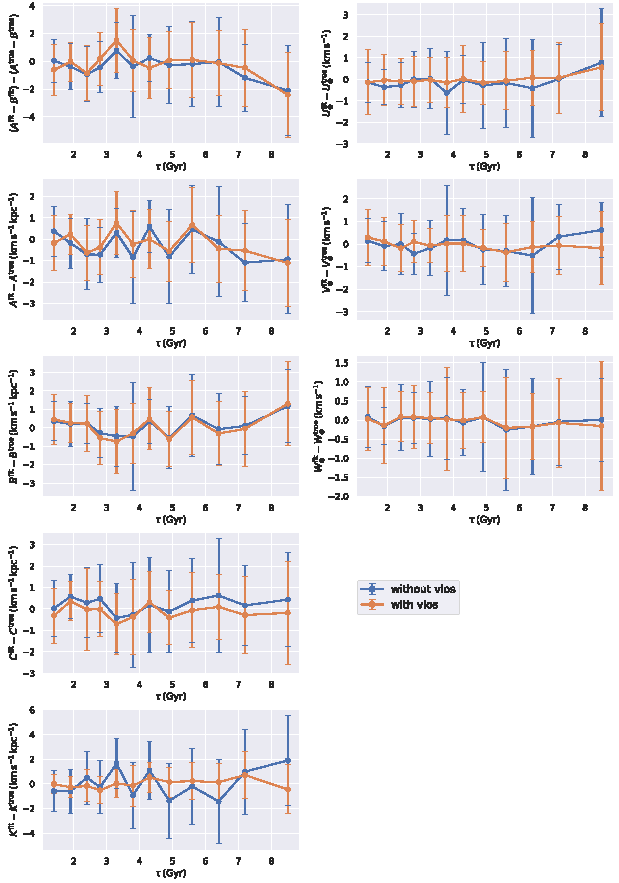
\includegraphics[width=15cm]{fig/Mock_vlos.pdf}
	\caption{視線速度の観測方程式有りと無しで解析したときの結果の絶対誤差、相対誤差と相対誤差のlogスケール。横軸は各パラメータとなっている。視線速度有りの解析の方が無しの解析よりも精度が高いことがわかる。右図は左図の結果の絶対誤差と相対誤差。} \label{fig:Mock_vlos}
\end{figure*}

%%%%%%%%%%%%%%%%%%%%%%%%%%%%%%%%%%%%%%%%%%%%%%%%%%%%%%%%%%%%%%%%%%%%%%%%%%%%%%%%%%%%%%%%%%%%%%%%
%%%%%%%%%%%%%%%%%%%%%%%%%%%%%%%%%%%%%%%%%%%%%%%%%%%%%%%%%%%%%%%%%%%%%%%%%%%%%%%%%%%%%%%%%%%%%%%%
%%%%%%%%%%%%%%%%%%%%%%%%%%%%%%%%%%%%%%%%%%%%%%%%%%%%%%%%%%%%%%%%%%%%%%%%%%%%%%%%%%%%%%%%%%%%%%%%

\subsection{解析3: 速度楕円体の傾きの解析結果への影響}
図\ref{fig:Mock_VE}は模擬データの速度$U$と$V$の間の速度楕円体の傾き$l_{UV}$を$0,10,20,30,40$度の5通りに設定した模擬データを生成し、それらをそれぞれ解析した結果である。この結果では$l_{UV}$の値による大きな違いは見られなかった。

\begin{figure*}[htbp]
	\centering
	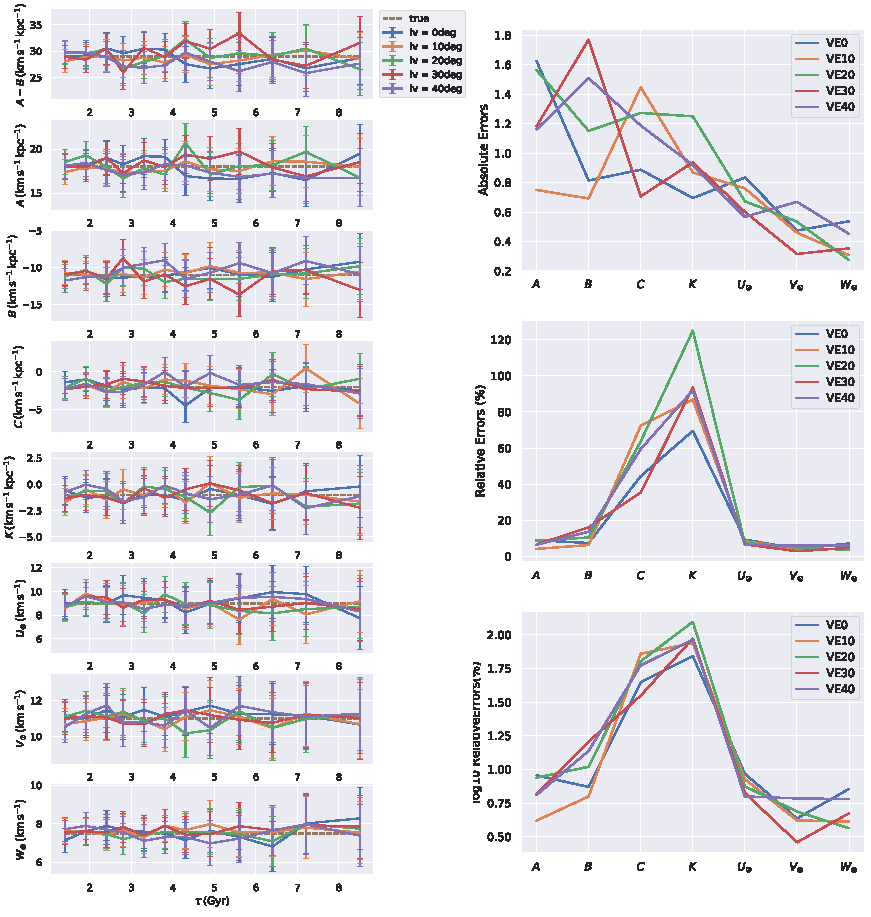
\includegraphics[width=15cm]{fig/Mock_VE.pdf}
	\caption{1000個の星の模擬データを速度楕円体の傾き$0,10,20,30,40$度で解析した結果。縦軸は各パラメータの値、横軸は模擬データに入れた速度分散に対応する年齢。} \label{fig:Mock_VE}
\end{figure*}


%%%%%%%%%%%%%%%%%%%%%%%%%%%%%%%%%%%%%%%%%%%%%%%%%%%%%%%%%%%%%%%%%%%%%%%%%%%%%%%%%%%%%%%%%%%%%%%%
%%%%%%%%%%%%%%%%%%%%%%%%%%%%%%%%%%%%%%%%%%%%%%%%%%%%%%%%%%%%%%%%%%%%%%%%%%%%%%%%%%%%%%%%%%%%%%%%
%%%%%%%%%%%%%%%%%%%%%%%%%%%%%%%%%%%%%%%%%%%%%%%%%%%%%%%%%%%%%%%%%%%%%%%%%%%%%%%%%%%%%%%%%%%%%%%%

\subsection{解析4: 太陽からの距離の解析結果への影響}
図\ref{fig:Mock_D}はサンプル星の太陽からの距離$D$の範囲を変えたときの解析結果である。$D<0.3\ \mathrm{kpc}$では他のパターンに比べて精度が悪い。
\begin{figure*}[htbp]
	\centering
	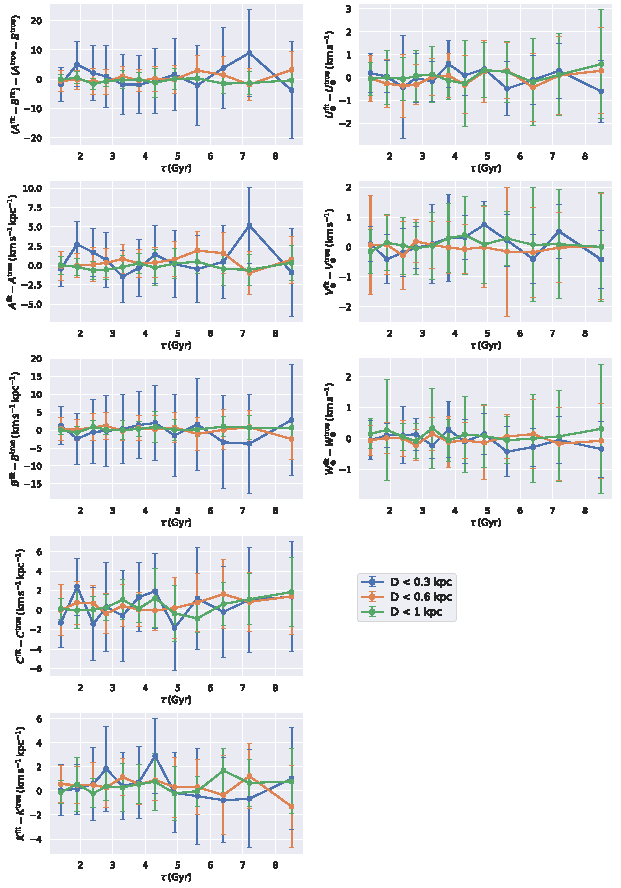
\includegraphics[width=15cm]{fig/Mock_D.pdf}
	\caption{1000個の星の模擬データを太陽からの距離を変えて$(D<0.3,0.4,,,1\  \mathrm{kpc})$解析した結果。縦軸は各パラメータの値、横軸は模擬データに入れた速度分散に対応する年齢。ラベルのD03は$D<0.3\ \mathrm{kpc}$、D04は$D<0.4\ \mathrm{kpc}$を意味する。} \label{fig:Mock_D}
\end{figure*}

%%%%%%%%%%%%%%%%%%%%%%%%%%%%%%%%%%%%%%%%%%%%%%%%%%%%%%%%%%%%%%%%%%%%%%%%%%%%%%%%%%%%%%%%%%%%%%%%
%%%%%%%%%%%%%%%%%%%%%%%%%%%%%%%%%%%%%%%%%%%%%%%%%%%%%%%%%%%%%%%%%%%%%%%%%%%%%%%%%%%%%%%%%%%%%%%%
%%%%%%%%%%%%%%%%%%%%%%%%%%%%%%%%%%%%%%%%%%%%%%%%%%%%%%%%%%%%%%%%%%%%%%%%%%%%%%%%%%%%%%%%%%%%%%%%

\subsection{解析5: 円盤面からの距離の解析結果への影響}
図\ref{fig:Mock_z}はサンプル星の円盤面からの距離$|z|$の範囲を変えて生成した模擬データの解析結果である。つまり、$|z|=100\ \mathrm{pc}$の場合、円盤面から$100\ \mathrm{pc}$以内の星を使用している。この解析結果からは$|z|$の値による大きな違いは見られなかった。

\begin{figure*}[htbp]
	\centering
	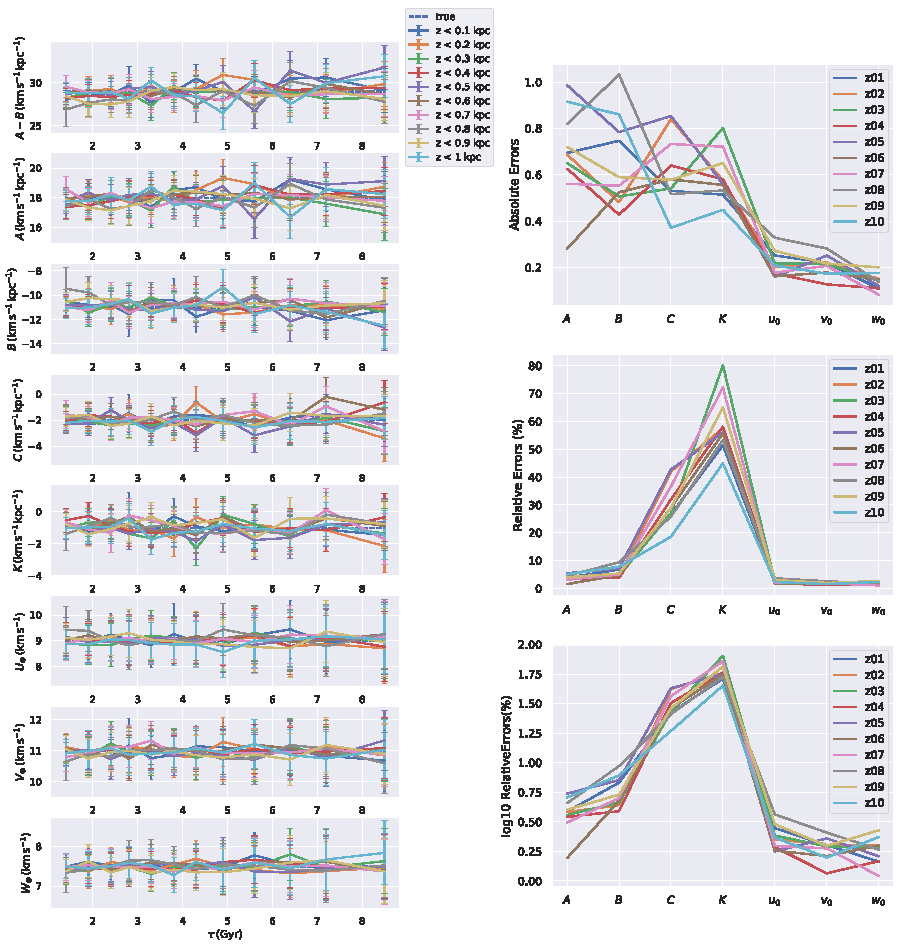
\includegraphics[width=15cm]{fig/Mock_z.pdf}
	\caption{1000個の星の模擬データを円盤面からの距離の範囲を変えて$(|z|<0.1,0.2,,,1 \mathrm{kpc})$解析した結果。縦軸は各パラメータの値、横軸は模擬データに入れた速度分散に対応する年齢。} \label{fig:Mock_z}
\end{figure*}

%%%%%%%%%%%%%%%%%%%%%%%%%%%%%%%%%%%%%%%%%%%%%%%%%%%%%%%%%%%%%%%%%%%%%%%%%%%%%%%%%%%%%%%%%%%%%%%%
%%%%%%%%%%%%%%%%%%%%%%%%%%%%%%%%%%%%%%%%%%%%%%%%%%%%%%%%%%%%%%%%%%%%%%%%%%%%%%%%%%%%%%%%%%%%%%%%
%%%%%%%%%%%%%%%%%%%%%%%%%%%%%%%%%%%%%%%%%%%%%%%%%%%%%%%%%%%%%%%%%%%%%%%%%%%%%%%%%%%%%%%%%%%%%%%%

\subsection{解析6: サンプル数の解析結果への影響}
\begin{figure*}[htbp]
	\centering
	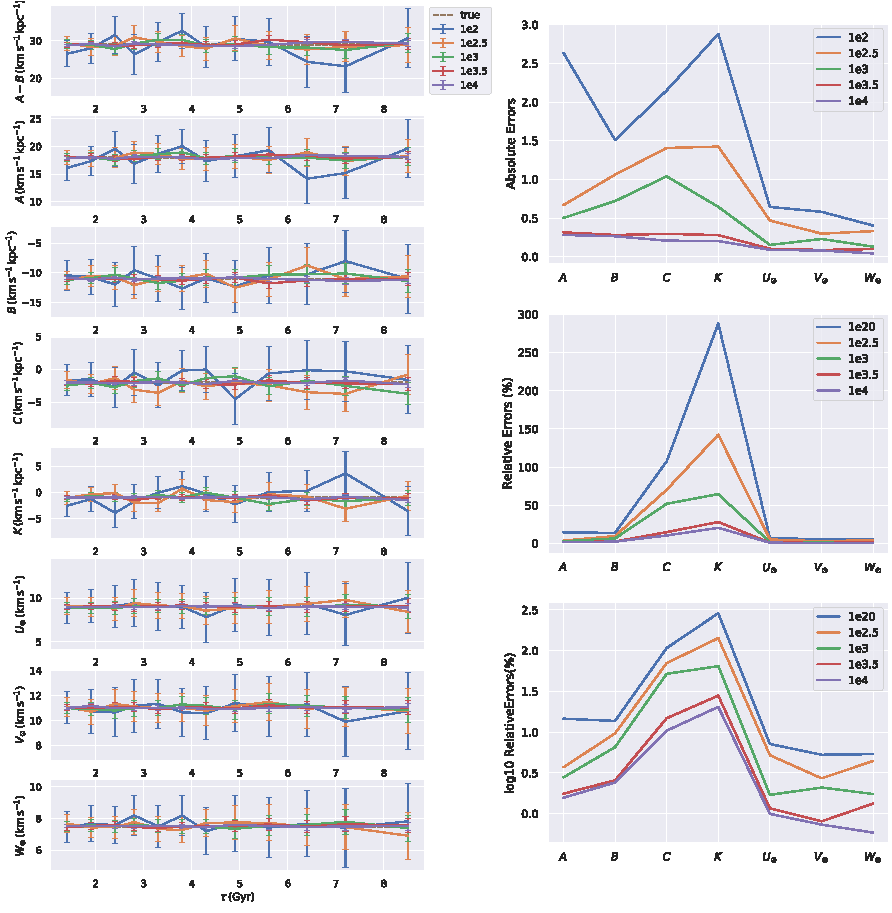
\includegraphics[width=15cm]{fig/Mock_N.pdf}
	\caption{サンプル数を変えて解析したときの結果の相対誤差。横軸は各パラメータ、縦軸は模擬データ生成時に設定した値と解析結果の値との相対誤差のlogスケール。サンプル数が多いほど相対誤差が小さくなっていることがわかる。} \label{fig:Mock_N}
\end{figure*}

%%%%%%%%%%%%%%%%%%%%%%%%%%%%%%%%%%%%%%%%%%%%%%%%%%%%%%%%%%%%%%%%%%%%%%%%%%%%%%%%%%%%%%%%%%%%%%%%
%%%%%%%%%%%%%%%%%%%%%%%%%%%%%%%%%%%%%%%%%%%%%%%%%%%%%%%%%%%%%%%%%%%%%%%%%%%%%%%%%%%%%%%%%%%%%%%%
%%%%%%%%%%%%%%%%%%%%%%%%%%%%%%%%%%%%%%%%%%%%%%%%%%%%%%%%%%%%%%%%%%%%%%%%%%%%%%%%%%%%%%%%%%%%%%%%

\subsection{解析7: $R_0$の値の解析結果への影響}
\begin{figure*}[htbp]
	\centering
	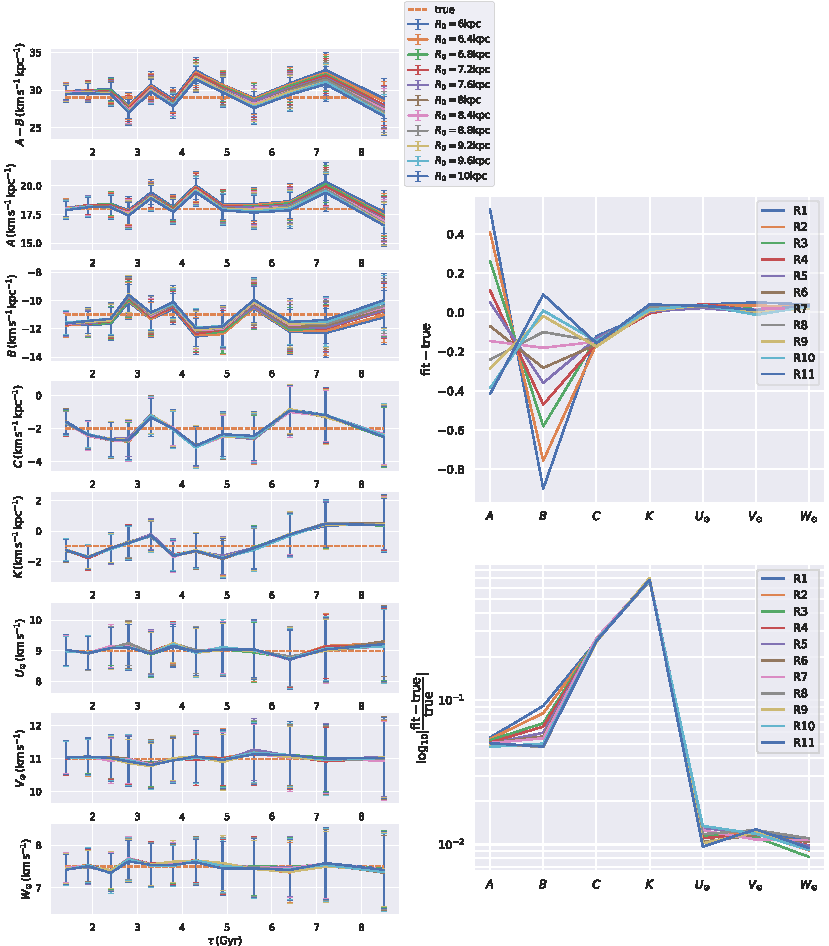
\includegraphics[width=15cm]{fig/Mock_R0.pdf}
	\caption{1000個の星の模擬データを太陽の銀河中心からの距離$R_0$を変えて$(R_0 = 6,6.4,6.8,,10 \mathrm{kpc})$解析した結果。縦軸は各パラメータの値、横軸は模擬データに入れた速度分散に対応する年齢。} \label{fig:Mock_R0}
\end{figure*}

\section{解析結果のまとめ}
全体的にオールト定数$C,K$の相対誤差が大きい結果となった。これは、これら2つのパラメータの絶対値がそれぞれ$2,1$と非常に小さいことが原因であると考えられる。また、顕著に見られる効果としてはasymmetric driftとサンプル数が大きい。サンプル数1000個の模擬データで$A,B,U_{\odot},V_{\odot},W_{\odot}$の相対誤差が10\%以下であることから、1000個のオーダーであれば銀河回転と太陽運動についてのパラメータについてはある程度の精度を確保できると考えられる。
\chapter{観測データ解析}

% Chap.4 観測データを用いたオールト解析 (仮)
% 4.1 使用する観測データ
%  4.1.1 観測データのカタログ ← Sanders & Das (2018) の説明
%  4.1.2 解析に使用するサンプル選定
% 4.2 観測データの解析結果 (仮)


\section{観測データ}
本研究では\cite{SD18}のカタログを用いて観測データの解析を行っている。このカタログはAPOGEE, Gaia-DSO, GALAH, LAMOST, RAVE, SEGUEの分光サーベイから利用できる分光パラメータとGaia Data Release 2 (DR2)で観測されたデータから約300万天体の距離、質量、年齢についての推定値を含むカタログとなっている。\cite{SD18}はisochrone fitにより分光データから年齢推定を行っており、年齢の不定性はAPOGEEで$\sim 16 \%$(最も正確な分光年齢推定)、GALAHで$\sim 21\%$、LAMOSTで$\sim 25\%$、RAVEとGESで$\sim 40\%$となっている。表\ref{spec_dataset}は彼らがカタログ生成の際に用いた分光データセットの表である。


\begin{table}[htb]
\small
\begin{center}
\scalebox{0.87}[0.9]{
\begin{tabular}{|l||c|c|c|c|c|} \hline
    観測 & 天体数 & 波長 & 分解能 & 使用したパラメータ & 測光データ\\ \hline
    APOGEE & 250万 & $H$バンド 15200 - 16900\AA & 22500 & $T_{\mathrm{eff}},\log g, \mathrm{[M/H]}$ & 2MASS\\
    LAMOST & 310万 & 可視光(3650 - 9000 \AA) & 1800 & $T_{\mathrm{eff}},\log g, \mathrm{[Fe/H]}$ & 2MASS \\
    RAVE & 50万 & 8400 - 8800 \AA & 7500 &   & 2MASS\\
    GES & & & 20000, 50000 & $T_{\mathrm{eff}},\log g, \mathrm{[Fe/H]}$ & VISTA, 2MASS\\
    GALAH & 26万 &  & 28000 & $T_{\mathrm{eff}},\log g, \mathrm{[Fe/H]}$ & 2MASS\\
    SEGUE & 19万 & 可視光 & 2000 & $T_{\mathrm{eff}},\log g, \mathrm{[Fe/H]}$ & 2MASS\\ \hline
\end{tabular}
}
\caption{\cite{SD18}のカタログで用いられた分光観測の種類、それぞれのデータの天体数、波長、分解能、年齢推定に使用したパラメータと測光データ。}
\end{center} \label{spec_dataset}
\end{table}

\begin{figure*}[htbp]
\begin{center}
	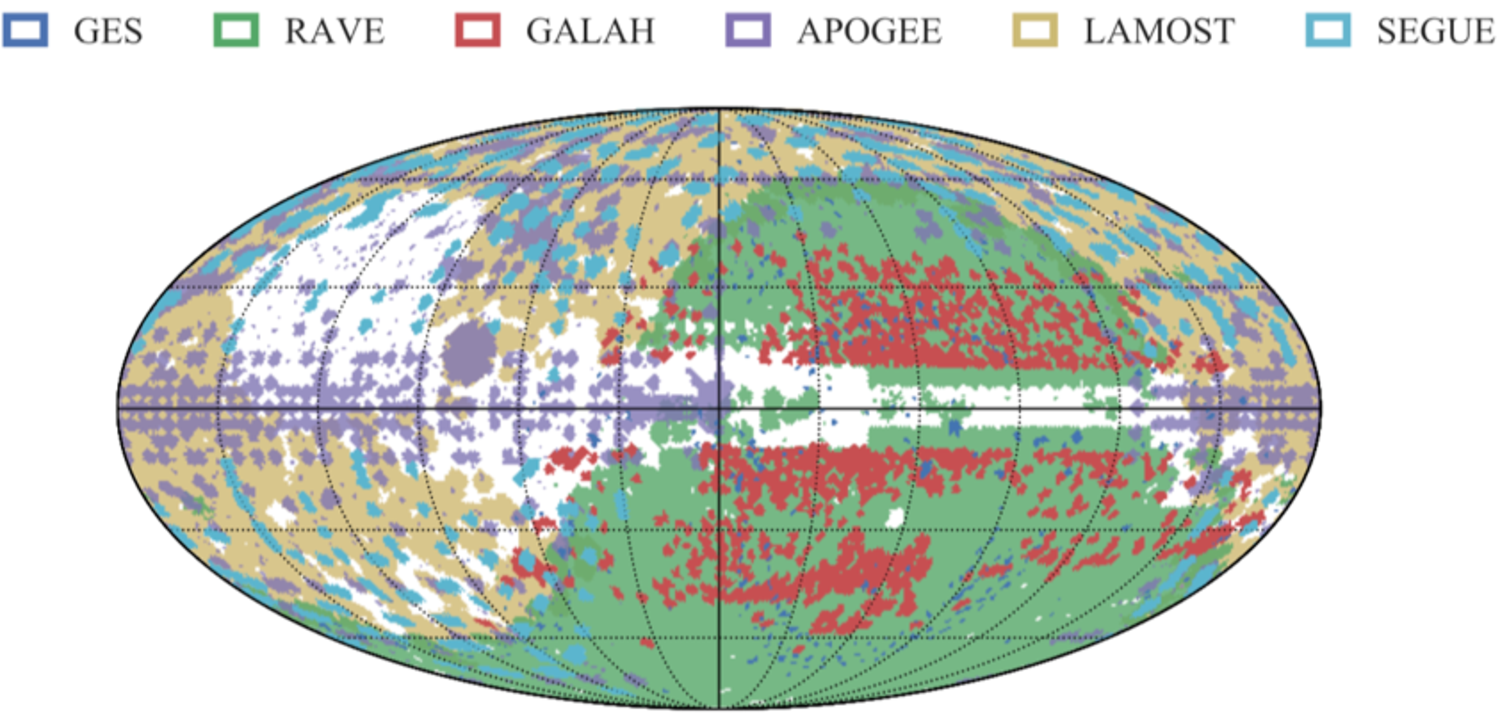
\includegraphics[width=9cm]{fig/SD18_fig1.pdf}
	\caption{\cite{SD18}で年齢推定がなされた星の分布。銀河を見たときのサーベイごとに色付けしている。}
	\label{fig2}
\end{center}
\end{figure*}

図\ref{mode_plx},\ref{mode_plx-age}はそれぞれ本研究で使用しているサンプルの年周視差$\varpi$ごとのモードと星の年齢$\tau$ごとのモードである。

\begin{figure*}[htbp]
\begin{center}
	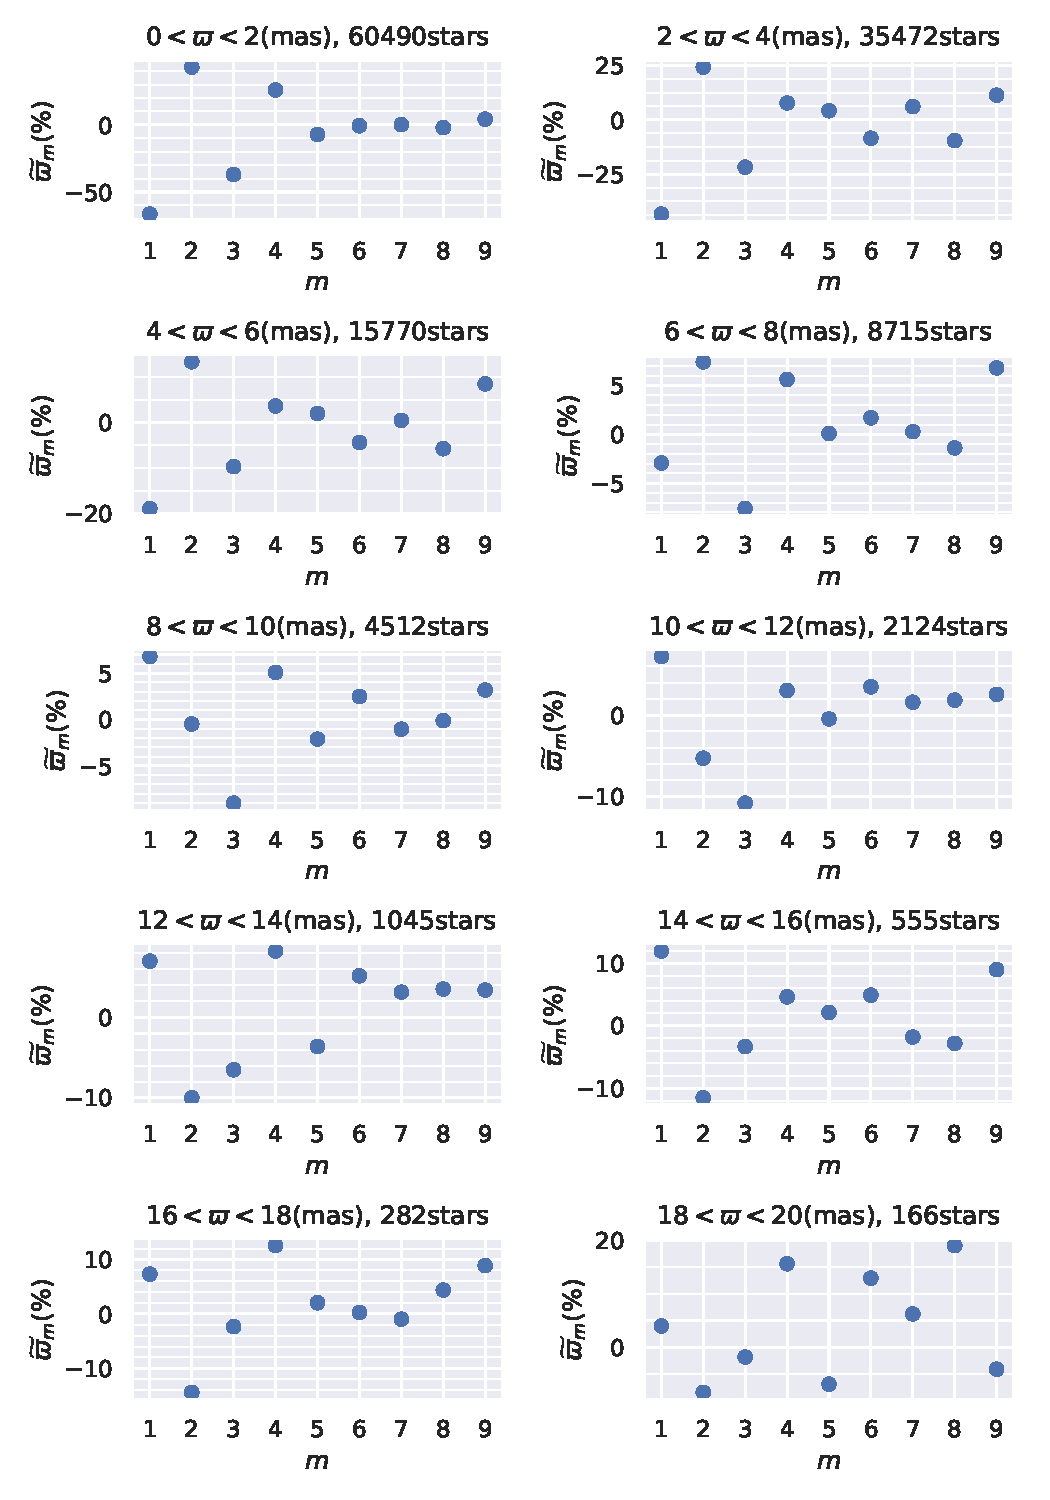
\includegraphics[width=12cm]{fig/mode_plx.pdf}
	\caption{今回使用しているサンプルの年周視差2 masごとのモード。各年周視差ごとのサンプルをフーリエ変換している。mはモードの係数である。}
	\label{mode_plx}
\end{center}
\end{figure*}

\begin{figure*}[htbp]
\begin{center}
	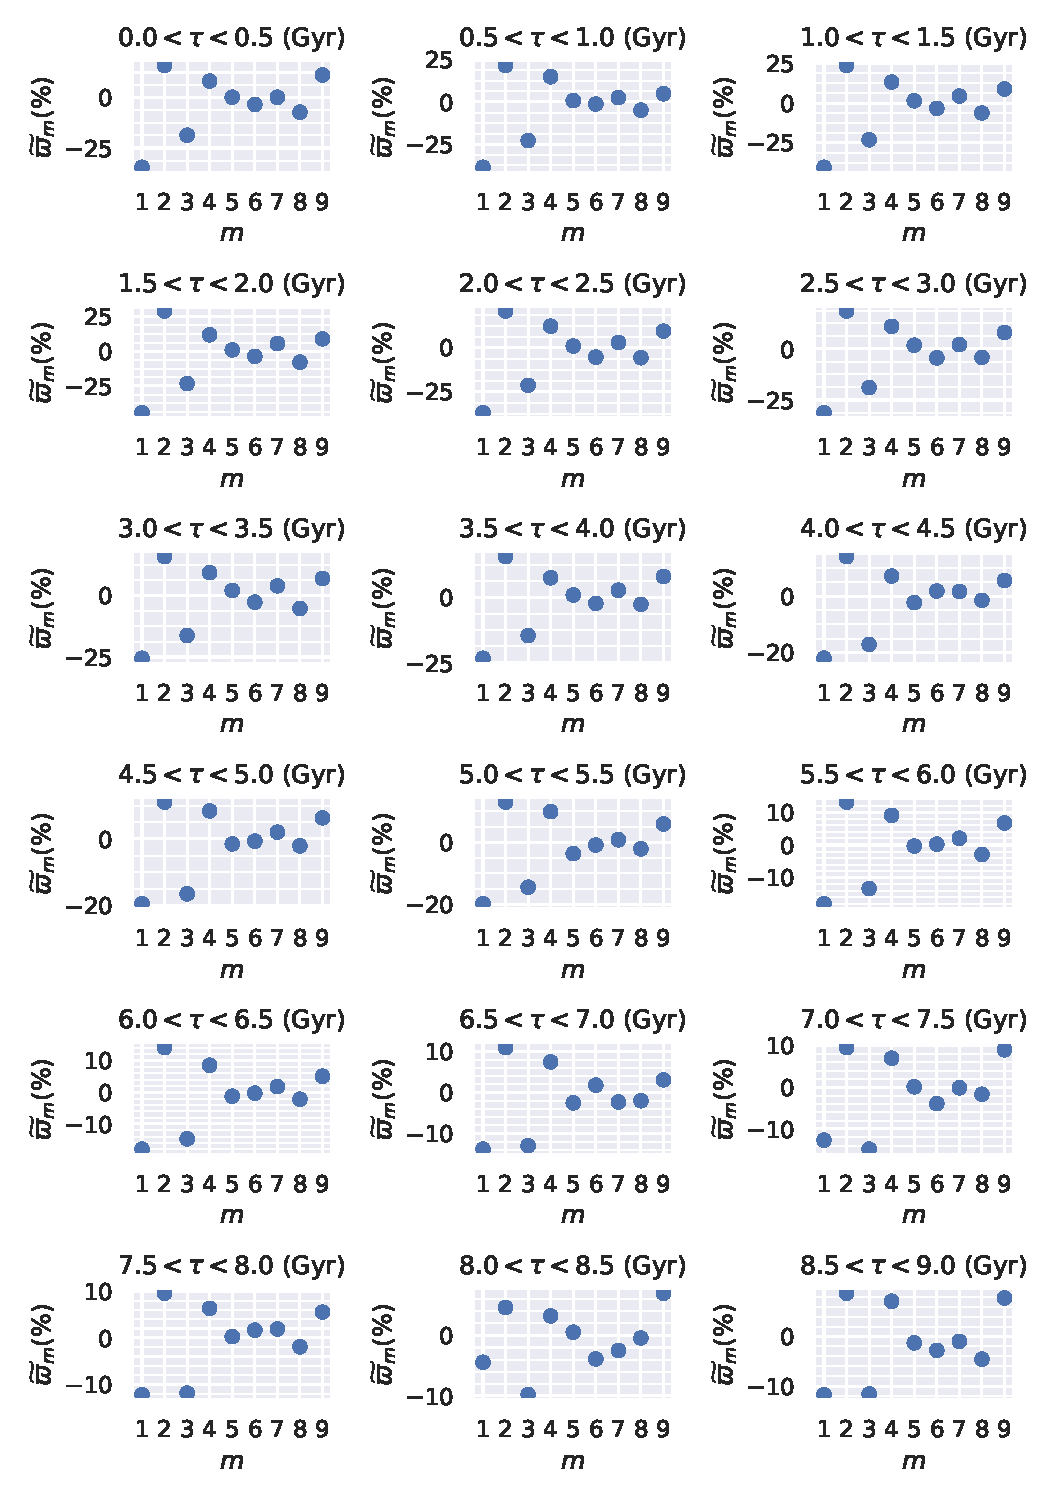
\includegraphics[width=14cm]{fig/mode_plx-age.pdf}
	\caption{太陽から1 kpc以内、年周視差の精度20\%以上、速度の観測誤差$3\ \mathrm{km\ s^{-1}}$以下の星の年齢0 Gyrから9 Gyrまでの0.5 Gyrごとのサンプルの年齢ごとのモード。mはモードの係数である。}
	\label{mode_plx-age}
\end{center}
\end{figure*}

図\ref{hist_seaborn_50Myr}, \ref{hist_seaborn_200Myr}, \ref{hist_seaborn_1Gyr}は星の年齢ごとの$U,V$の2次元速度分布である。$|z|<100\ \mathrm{pc}$のサンプルを使用している。

\begin{figure*}[htbp]
\begin{center}
	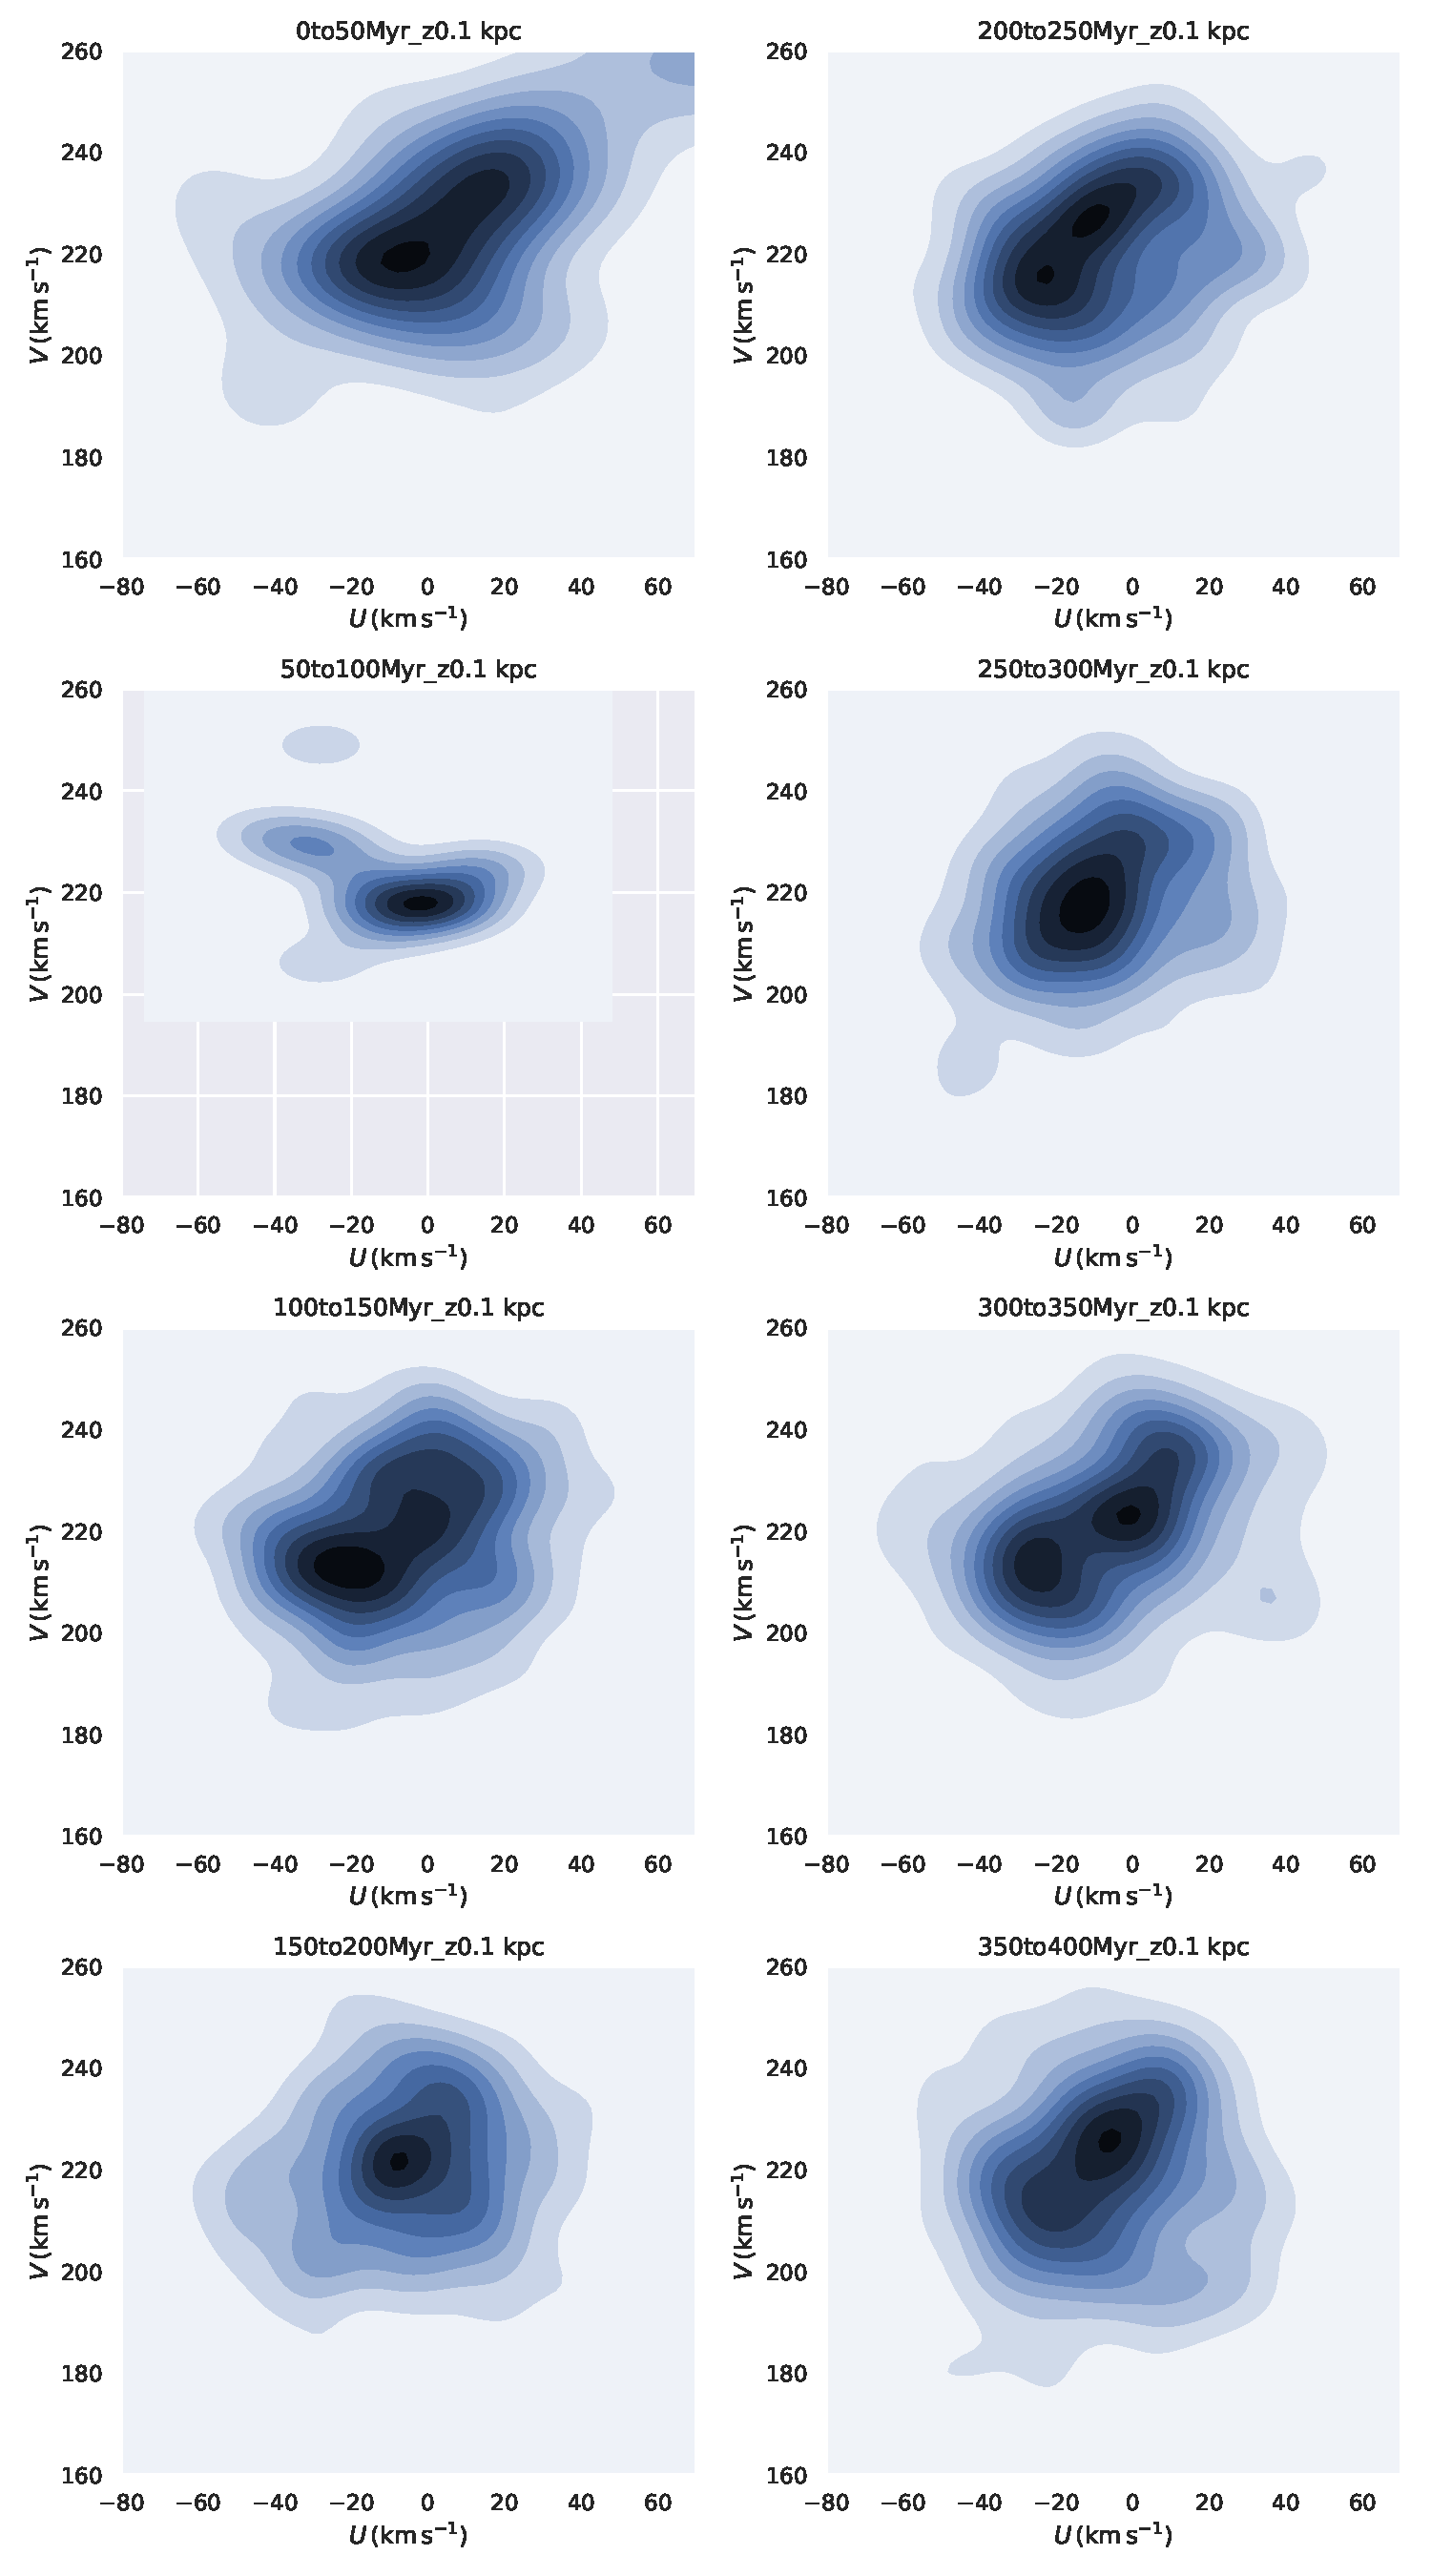
\includegraphics[width=12cm]{fig/UV/hist_seaborn_2_z0.1kpc.pdf}
	\caption{太陽から1 kpc以内、年周視差の精度20\%以上、速度の観測誤差$3\ \mathrm{km\ s^{-1}}$以下の星の年齢50 Myrごとの動径方向速度$U$、方位角方向速度$V$の分布。}
	\label{hist_seaborn_50Myr}
\end{center}
\end{figure*}

\begin{figure*}[htbp]
\begin{center}
	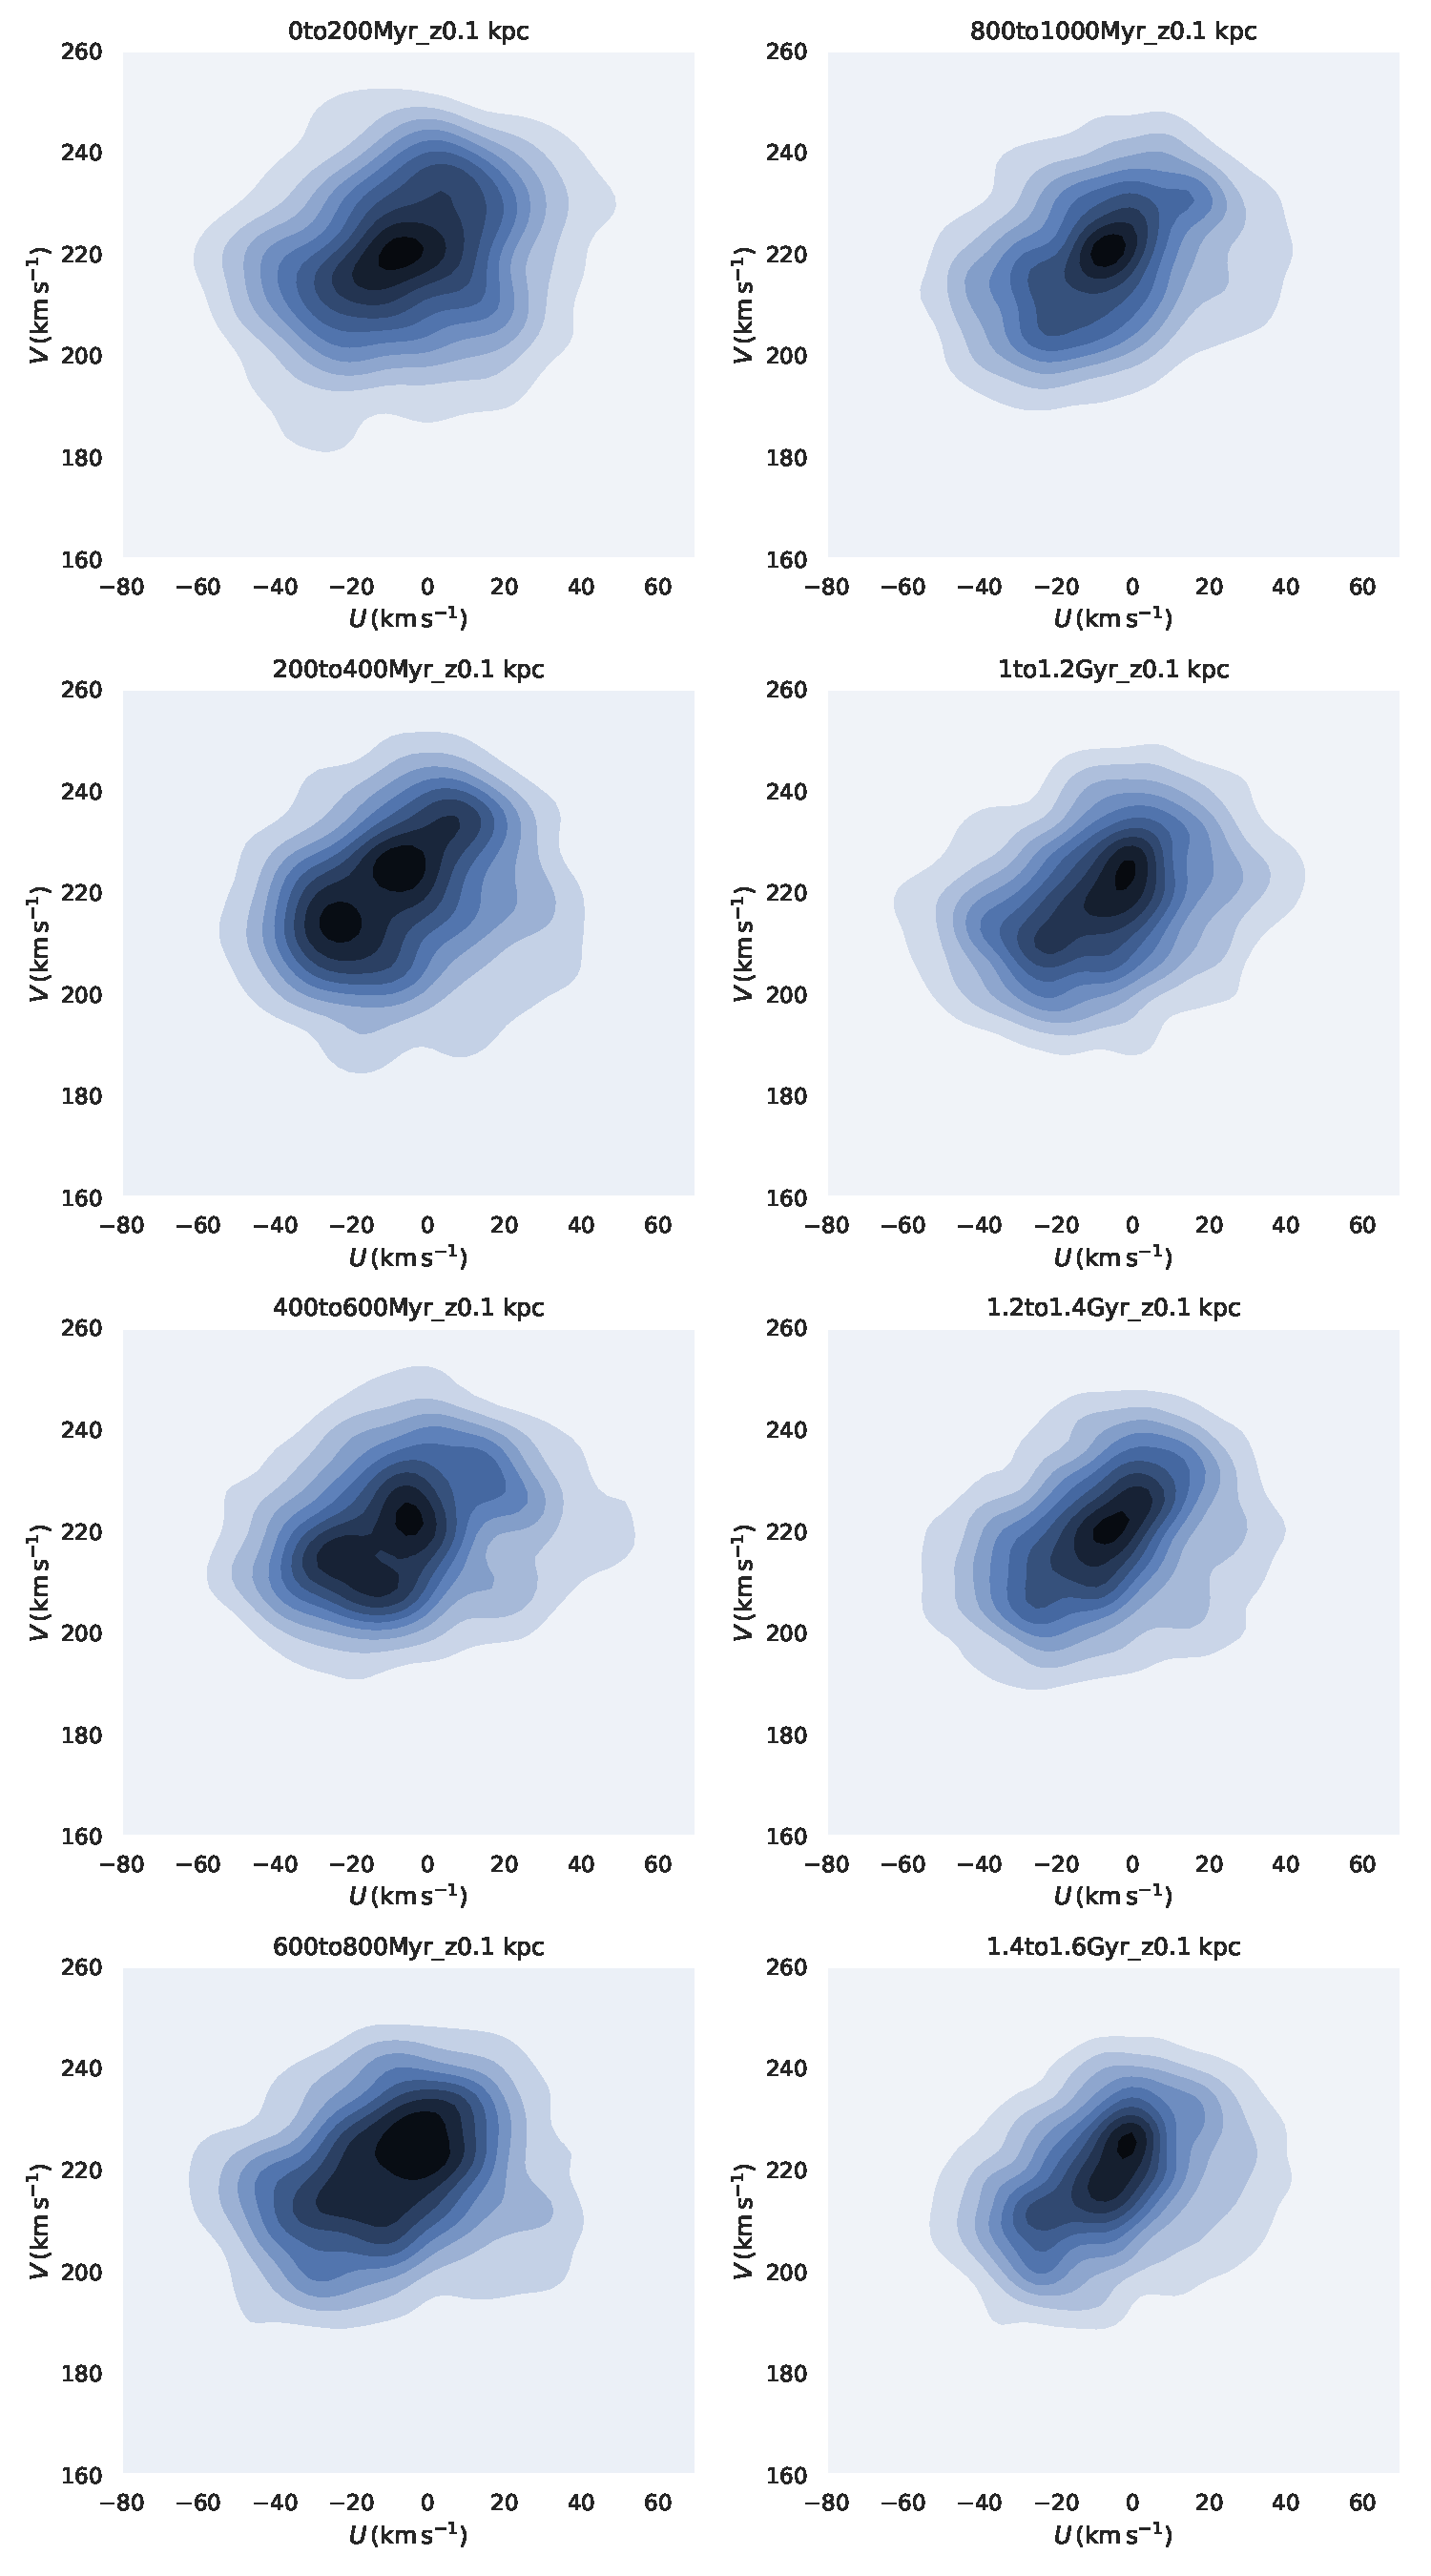
\includegraphics[width=12cm]{fig/UV/hist_seaborn_1_z0.1kpc.pdf}
	\caption{太陽から1 kpc以内、年周視差の精度20\%以上、速度の観測誤差$3\ \mathrm{km\ s^{-1}}$以下の星の年齢200 Myrごとの動径方向速度$U$、方位角方向速度$V$の分布。}
	\label{hist_seaborn_200Myr}
\end{center}
\end{figure*}

\begin{figure*}[htbp]
\begin{center}
	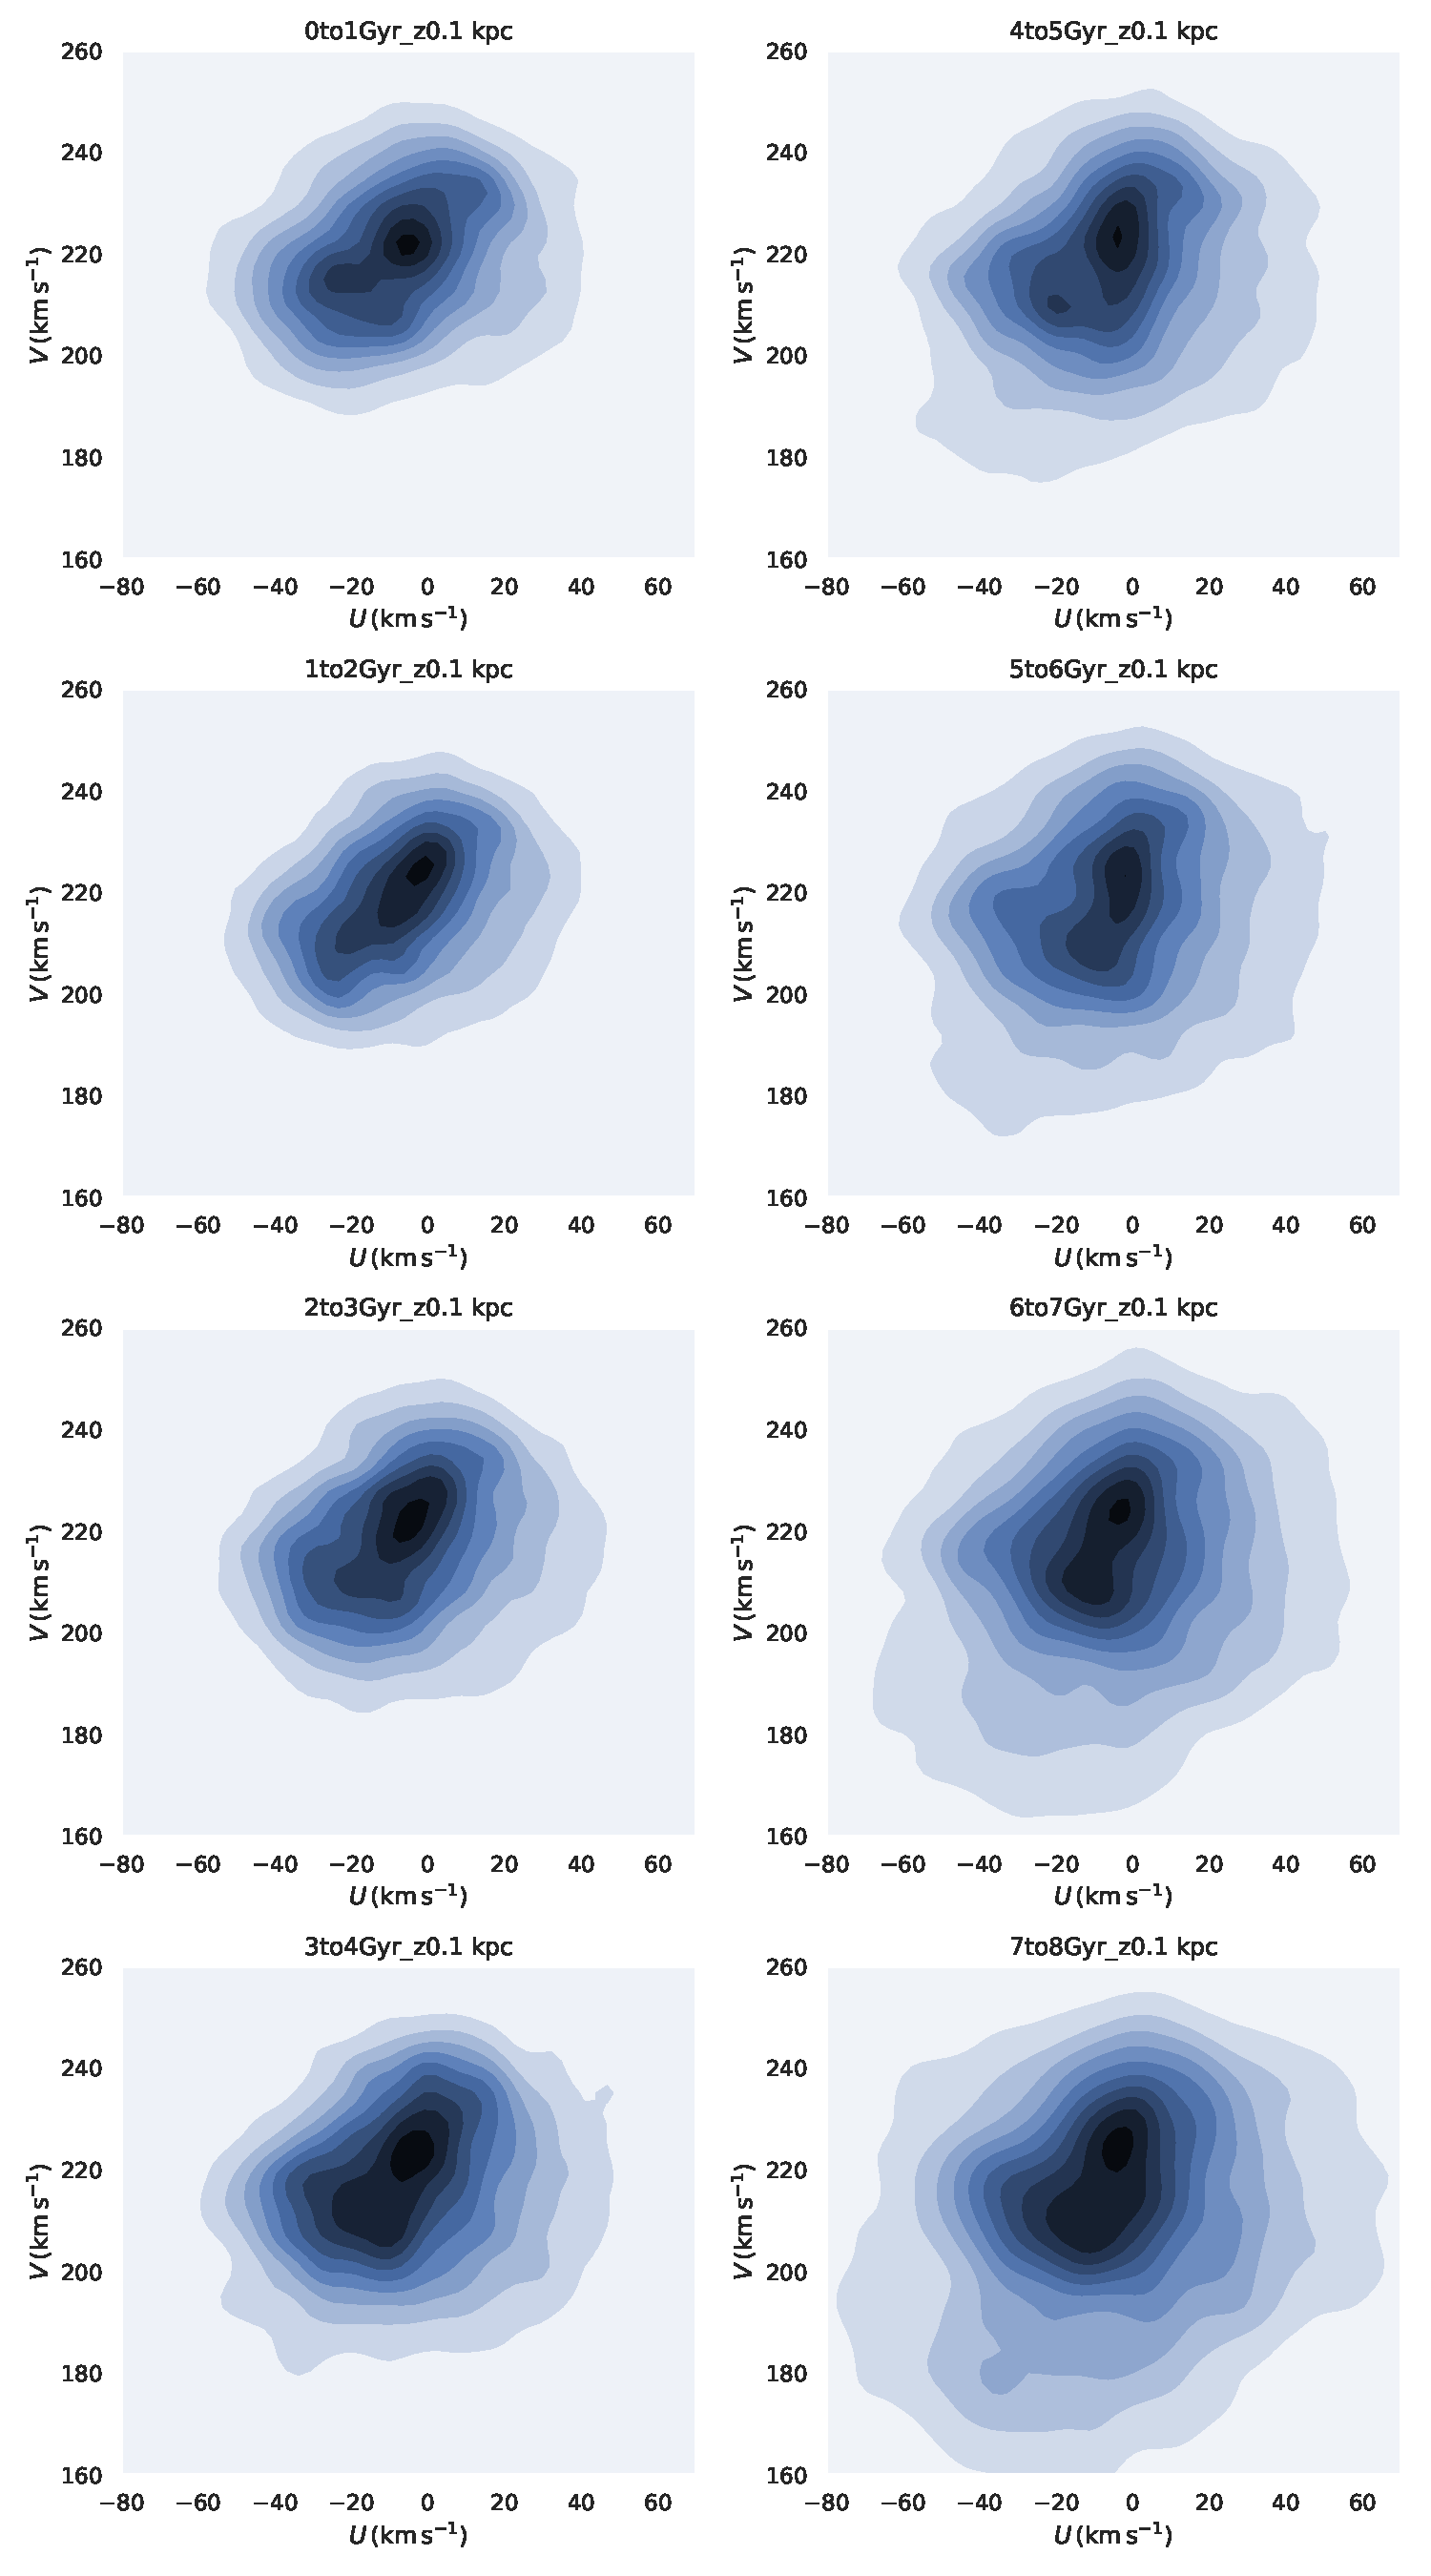
\includegraphics[width=12cm]{fig/UV/hist_seaborn_0_z0.1kpc.pdf}
	\caption{太陽から1 kpc以内、年周視差の精度20\%以上、速度の観測誤差$3\ \mathrm{km\ s^{-1}}$以下の星の年齢1 Gyrごとの動径方向速度$U$、方位角方向速度$V$の分布。}
	\label{hist_seaborn_1Gyr}
\end{center}
\end{figure*}

図\ref{hist_UV_50Myr}, \ref{hist_UV_200Myr}, \ref{hist_UV_1Gyr}は図\ref{hist_seaborn_50Myr}, \ref{hist_seaborn_200Myr}, \ref{hist_seaborn_1Gyr}をプロット方法を変えてプロットした図である。

\begin{figure*}[htbp]
   \centering
\begin{tabular}{cc}
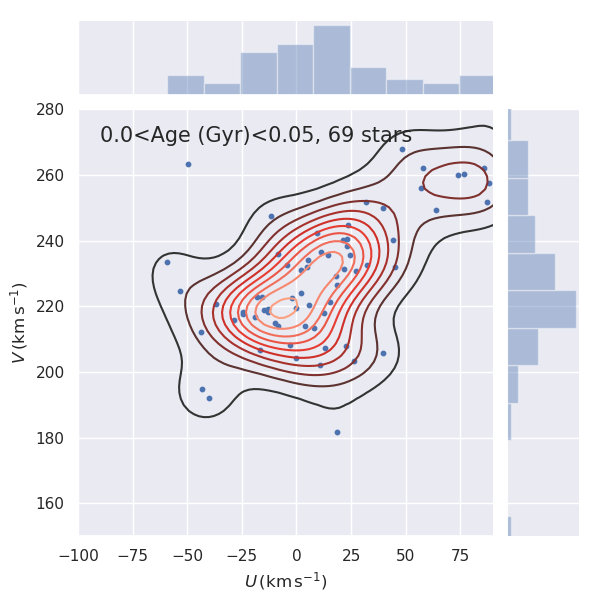
\includegraphics[width=5cm]{fig/UV/0to50Myr_z0.1kpc_hist2d.png}&
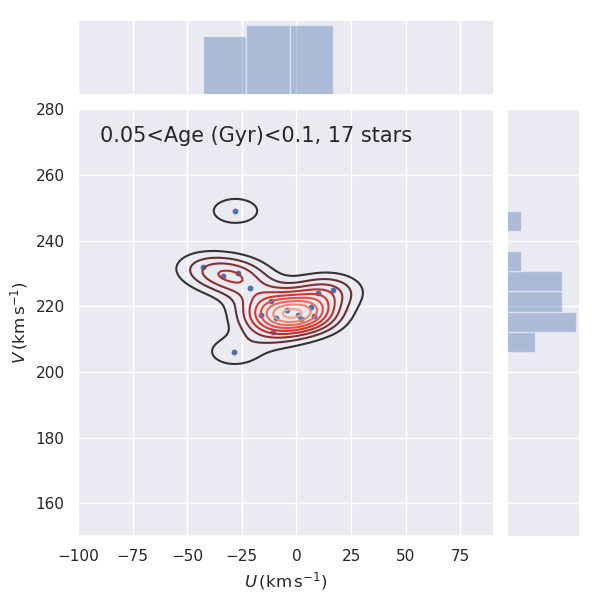
\includegraphics[width=5cm]{fig/UV/50to100Myr_z0.1kpc_hist2d.png}\\
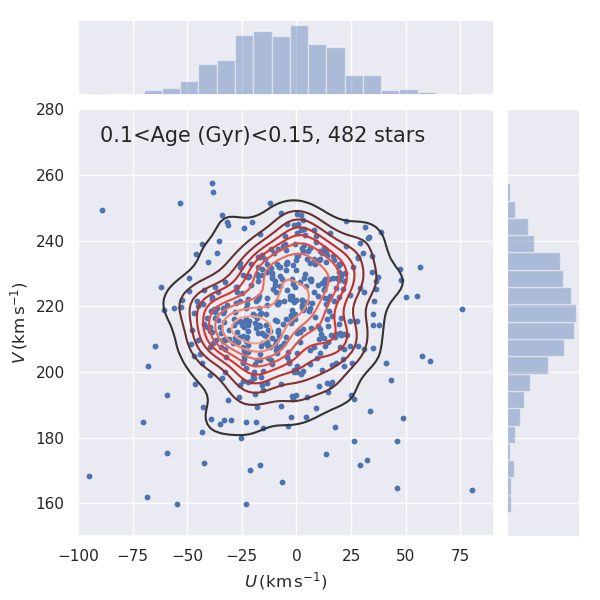
\includegraphics[width=5cm]{fig/UV/100to150Myr_z0.1kpc_hist2d.png}&
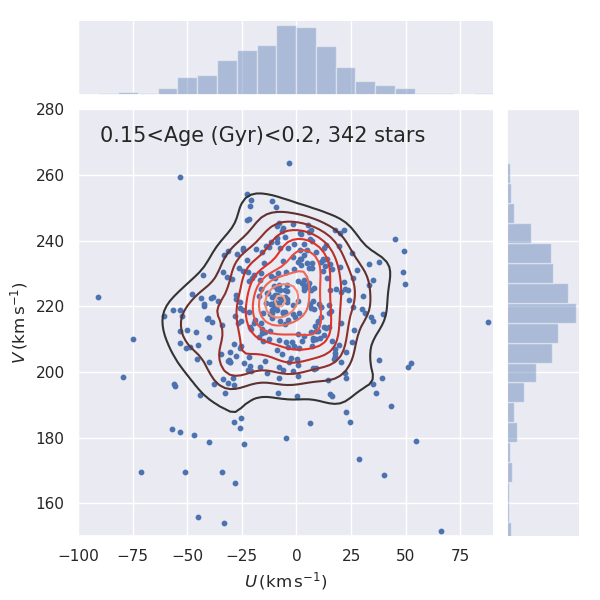
\includegraphics[width=5cm]{fig/UV/150to200Myr_z0.1kpc_hist2d.png}\\
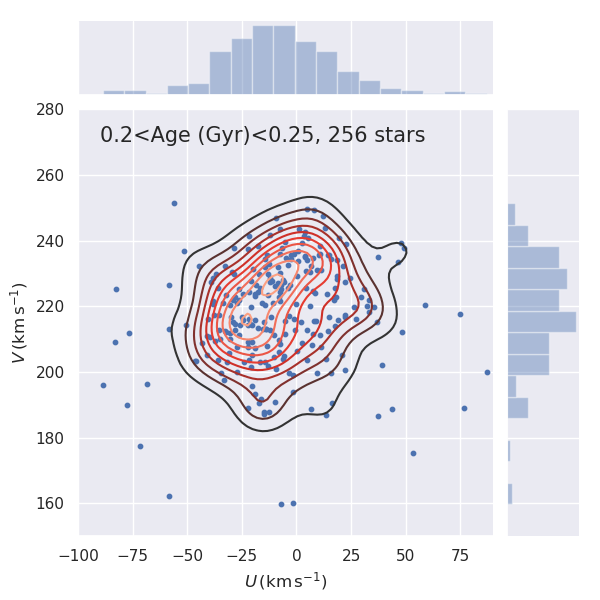
\includegraphics[width=5cm]{fig/UV/200to250Myr_z0.1kpc_hist2d.png}&
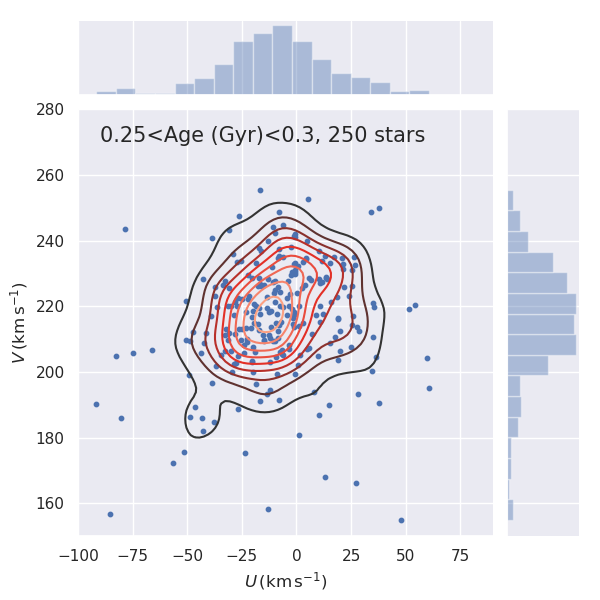
\includegraphics[width=5cm]{fig/UV/250to300Myr_z0.1kpc_hist2d.png}\\
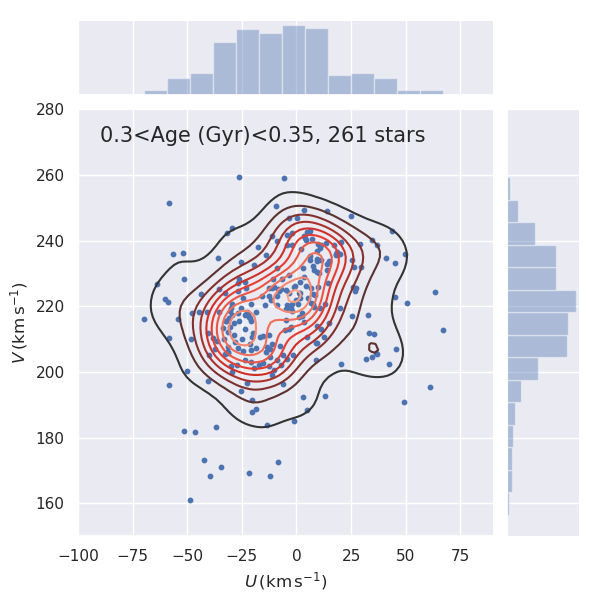
\includegraphics[width=5cm]{fig/UV/300to350Myr_z0.1kpc_hist2d.png}&
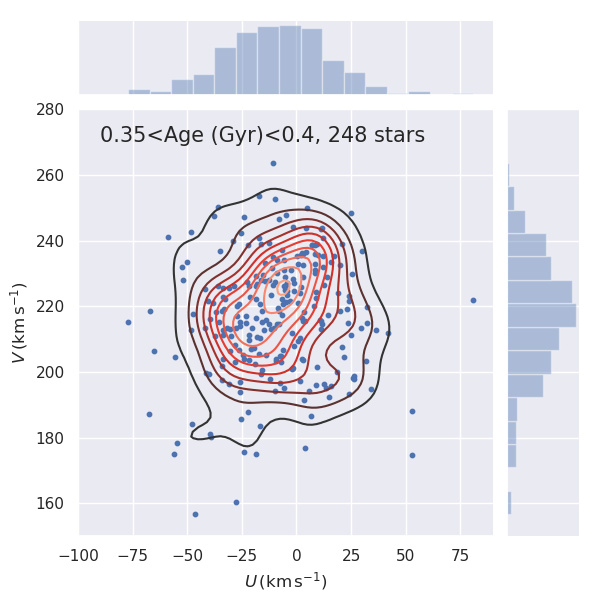
\includegraphics[width=5cm]{fig/UV/350to400Myr_z0.1kpc_hist2d.png}\\
\end{tabular}
    \caption{太陽から1 kpc以内、年周視差の精度20\%以上、速度の観測誤差$3\ \mathrm{km\ s^{-1}}$以下の星の年齢50 Myrごとの動径方向速度$U$、方位角方向速度$V$の分布。}
    \label{hist_UV_50Myr}
\end{figure*}

\begin{figure*}[htbp]
   \centering
\begin{tabular}{cc}
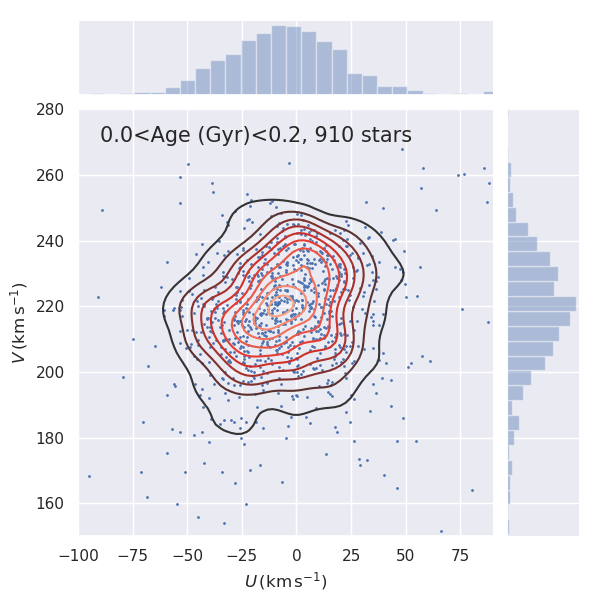
\includegraphics[width=5cm]{fig/UV/0to200Myr_z0.1kpc_hist2d.png}&
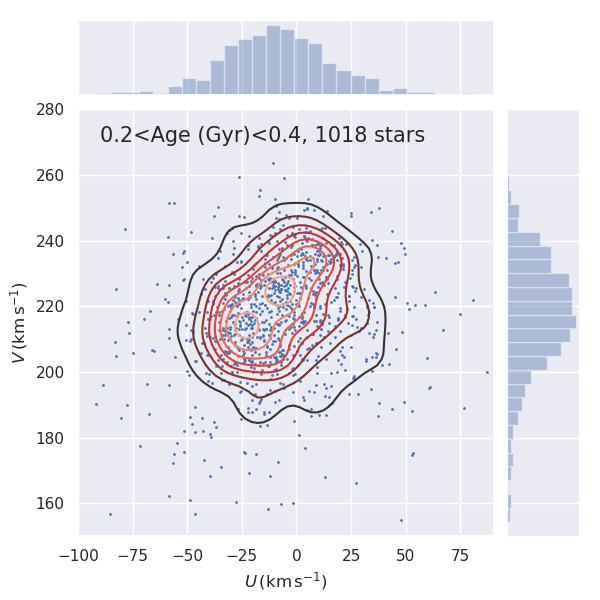
\includegraphics[width=5cm]{fig/UV/200to400Myr_z0.1kpc_hist2d.png}\\
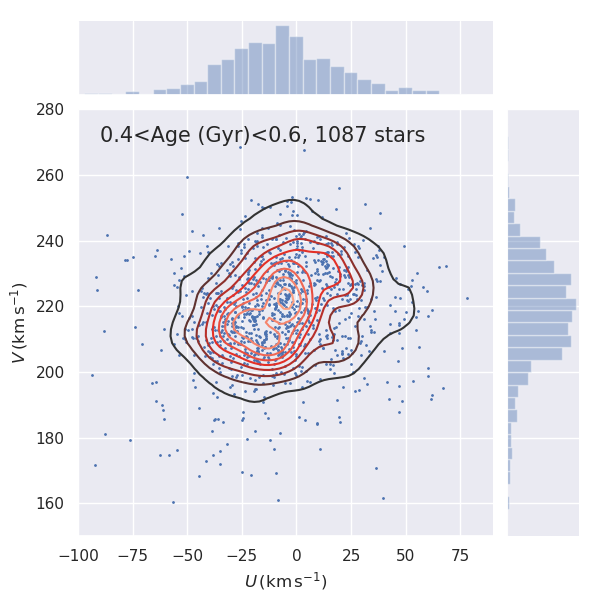
\includegraphics[width=5cm]{fig/UV/400to600Myr_z0.1kpc_hist2d.png}&
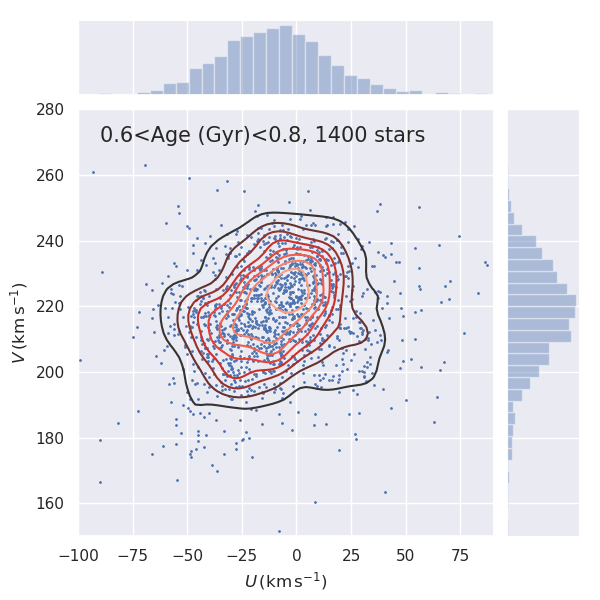
\includegraphics[width=5cm]{fig/UV/600to800Myr_z0.1kpc_hist2d.png}\\
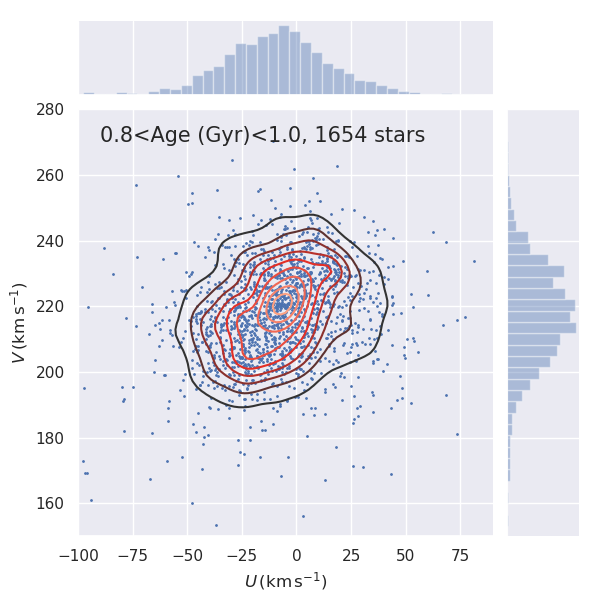
\includegraphics[width=5cm]{fig/UV/800to1000Myr_z0.1kpc_hist2d.png}&
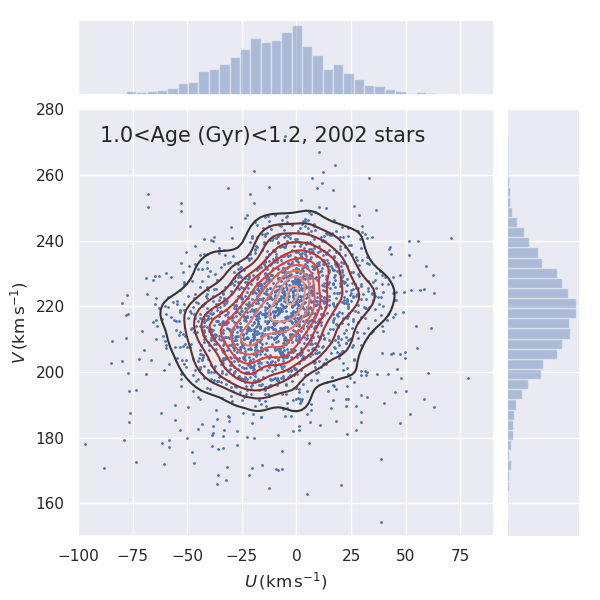
\includegraphics[width=5cm]{fig/UV/1to1.2Gyr_z0.1kpc_hist2d.png}\\
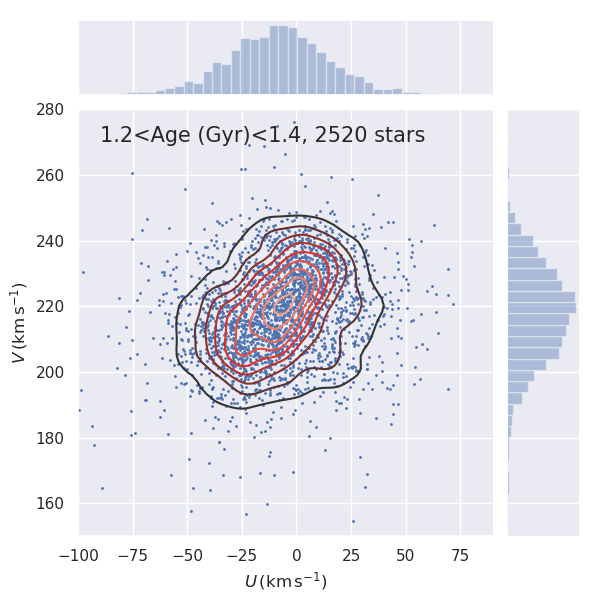
\includegraphics[width=5cm]{fig/UV/1.2to1.4Gyr_z0.1kpc_hist2d.png}&
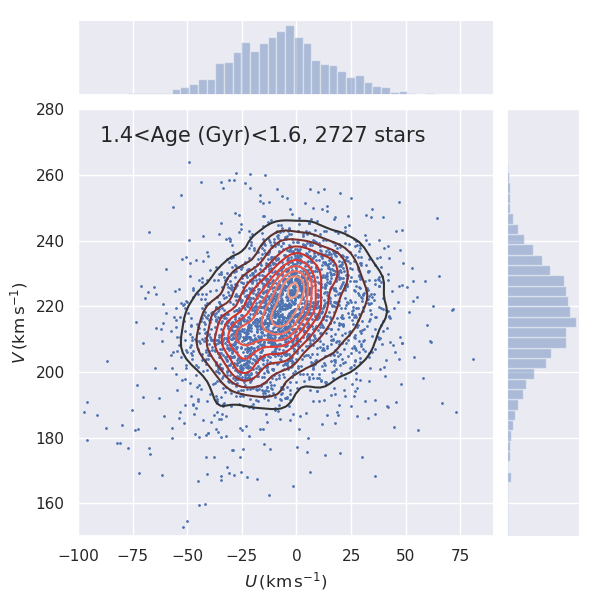
\includegraphics[width=5cm]{fig/UV/1.4to1.6Gyr_z0.1kpc_hist2d.png}\\
\end{tabular}
    \caption{太陽から1 kpc以内、年周視差の精度20\%以上、速度の観測誤差$3\ \mathrm{km\ s^{-1}}$以下の星の年齢200 Myrごとの動径方向速度$U$、方位角方向速度$V$の分布。}
    \label{hist_UV_200Myr}
\end{figure*}

\begin{figure*}[htbp]
   \centering
\begin{tabular}{cc}
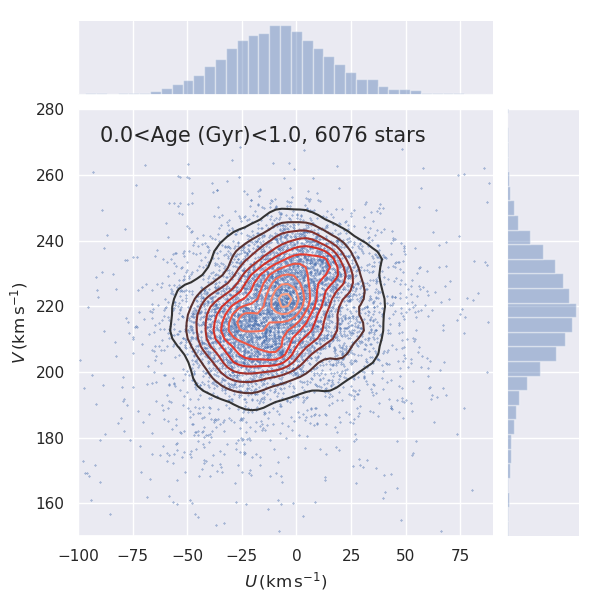
\includegraphics[width=5cm]{fig/UV/0to1Gyr_z0.1kpc_hist2d.png}&
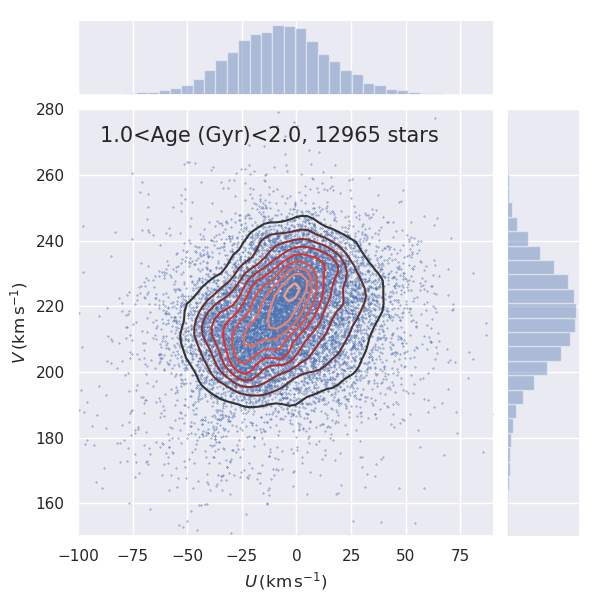
\includegraphics[width=5cm]{fig/UV/1to2Gyr_z0.1kpc_hist2d.png}\\
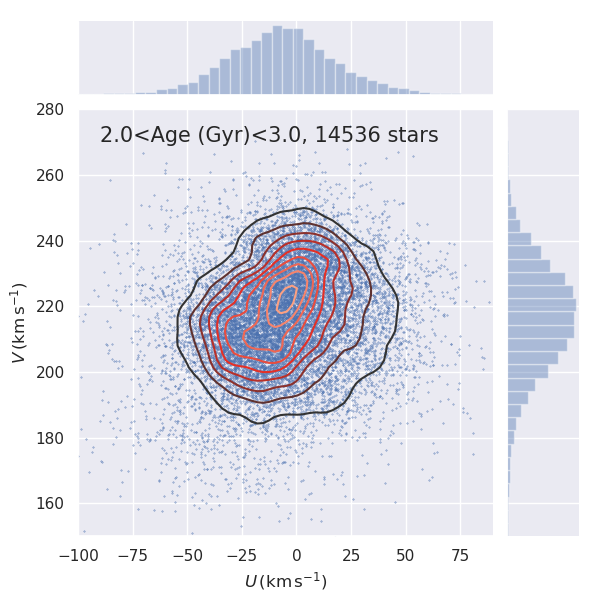
\includegraphics[width=5cm]{fig/UV/2to3Gyr_z0.1kpc_hist2d.png}&
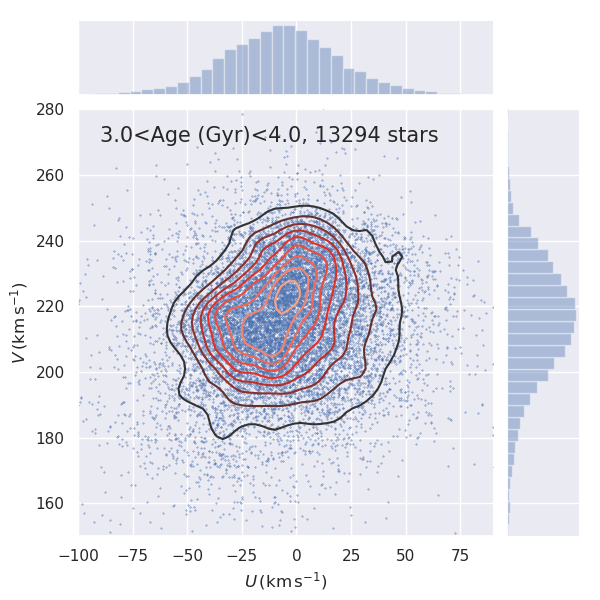
\includegraphics[width=5cm]{fig/UV/3to4Gyr_z0.1kpc_hist2d.png}\\
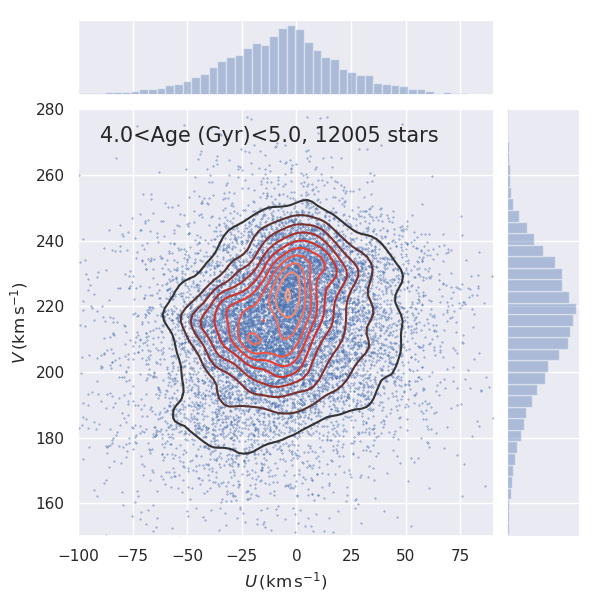
\includegraphics[width=5cm]{fig/UV/4to5Gyr_z0.1kpc_hist2d.png}&
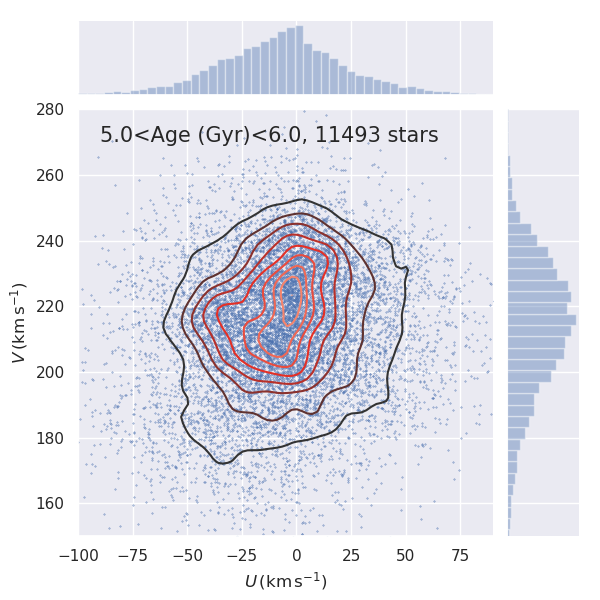
\includegraphics[width=5cm]{fig/UV/5to6Gyr_z0.1kpc_hist2d.png}\\
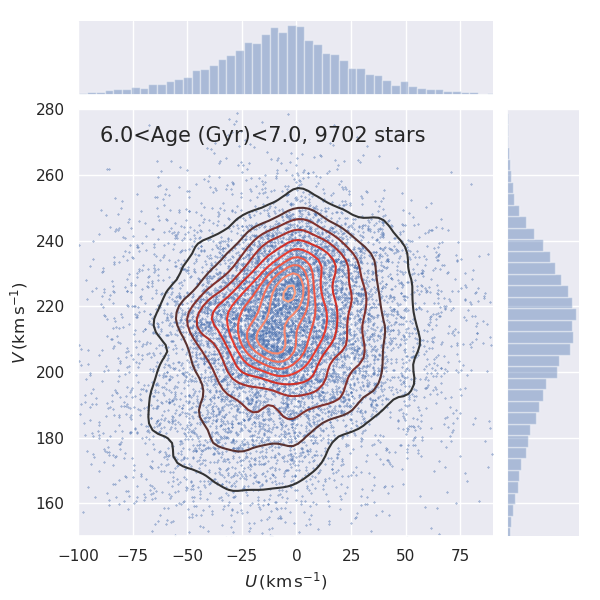
\includegraphics[width=5cm]{fig/UV/6to7Gyr_z0.1kpc_hist2d.png}&
\includegraphics[width=5cm]{fig/UV/7to8Gyr_z0.1kpc_hist2d.png}\\
\end{tabular}
    \caption{太陽から1 kpc以内、年周視差の精度20\%以上、速度の観測誤差$3\ \mathrm{km\ s^{-1}}$以下の星の年齢1 Gyrごとの動径方向速度$U$、方位角方向速度$V$の分布。}
    \label{hist_UV_1Gyr}
\end{figure*}


\subsection{使用するサンプル}
年周視差の相対誤差は$\varpi/\sigma_{\varpi}>5$として、20 $\%$未満としている(\cite{BJ15})。速度の観測誤差は、$\mu_l,\mu_b,v_{\mathrm{los}},\varpi$の誤差伝播を考慮して3次元速度ベクトル$v_{\mathrm{Total}}$とし、またその誤差も同様に計算して$\sigma_{v_{\mathrm{Total}}}3\mathrm{km\,s^{-1}}$と制限している。本研究で用いているOort-Lindbladモデルは冷たい系を考えているため、薄い円盤星(thin disk star)に適用したい。そのため、金属量[Fe/H]$>-0.2\,\mathrm{dex})$、円盤面からの距離$|z|<100\,\mathrm{pc}$、星の年齢$\tau < 8\,\mathrm{Gyr}$のデータを用いている。星の年齢でサンプルを制限する理由は、サンプル数が少ないことと、分散が非常に大きいためである。図\ref{fig:v_sigma}はサンプルの速度と速度分散のプロットである。0 - 1 Gyrでは2 Gyrより古い星と比べて速度$\overline{V}$と速度分散の各成分で異なる傾向が見られる。表\ref{dataset}は、以上の制限をしたときのサンプル数である。

また、この観測データ解析では太陽から銀河中心までの距離は$R_0 = 8.2\pm 0.1\ \mathrm{kpc}$(\cite{BH2016})としている。また、VLBIの観測(\cite{RB04},\cite{Reid08})からいて座A$^*$に対する太陽の接線速度は$\Omega_{g,\odot} = 30.24 \pm 0.12\ \mathrm{km\ s^{-1}\ kpc^{-1}}$としている。



\begin{table}[htb]
\small
\begin{center}
\scalebox{0.87}[0.9]{
\begin{tabular}{|l|cccccccc|} \hline
    星の年齢 (Gyr) & 0 - 1 & 1 - 2 & 2 - 3 & 3 - 4 & 4 - 5 & 5 - 6 & 6 - 7 & 7 - 8\\ \hline
    $D<600\ \mathrm{pc}$のサンプル数& 4096 & 7506 & 10241 & 10416 & 9861 & 9813 & 8426 & 7716\\
    $D<700\ \mathrm{pc}$のサンプル数 & 4601 & 9044 & 11587 & 11354 & 10631 & 10480 & 8939 & 8152\\
    $D<800\ \mathrm{pc}$のサンプル数 & 5127 & 10471 & 12746 & 12134 & 11235 & 10936 & 9287 & 8436\\
    $D<900\ \mathrm{pc}$のサンプル数 & 5615 & 11821 & 13716 & 12782 & 11702 & 11283 & 9557 & 8658\\
    $D<1\ \mathrm{kpc}$のサンプル数  & 6076 & 12965 & 14537 & 13296 & 12036 & 11554 & 9768 & 8821\\ \hline
\end{tabular}
}
\caption{使用したサンプルの星の年齢と太陽からの距離の範囲でのそれぞれのサンプル数}
\end{center} \label{dataset}
\end{table}


\begin{figure*}[htbp]
	\centering
	\includegraphics[width=15cm]{fig/v_sigma.pdf}
	\caption{\cite{SD18}のカタログの円筒座標系での速度と速度分散。サンプルの星の年齢を0 - 1 Gyr, 1 - 2 Gyrのように8 Gyrまでで区切っている。左側の列は各年齢での平均速度、右側の列は各年齢での速度分散の値。それぞれの線は使用したサンプルの太陽からの距離の範囲の違いである。600 pcから1 kpcまで100 pc刻みで範囲を制限している。それぞれのサンプルでほとんど違いはない。}
	\label{fig:v_sigma}
\end{figure*}


\section{観測データの解析結果}
観測データの解析結果を示す。本研究では、大きく分けてasymmetirc drifを考慮しない従来の観測方程式(\ref{ObsEq})での解析と考慮した観測方程式(\ref{ObsEqAD})の2種類で観測データ解析を行った。


\subsection{asymmetric driftを考慮しない解析}
図\ref{fig:woAD}は観測データにasymmetric driftを考慮しないときの観測方程式(\ref{ObsEq})を用いた解析の結果を示す。オールト定数$A,B$は太陽からの距離$D$の範囲ごとで値が0.5程度変わっている。太陽運動の銀河回転方向$V_{\odot}$は明らかに年齢依存性を持っていることがわかる。その値は0 - 1 Gyrと7 - 8 Gyrで約$6\ \mathrm{km\ s^{-1}}$増えており、1 Gyr増えるごとに約$0.75\ \mathrm{km\ s^{-1}}$増えることになる。また、オールト定数$C$は3 - 4 Gyrから4 - 5 Gyrにかけて$4\ \mathrm{km\ s^{-1}kpc}$減少している。$K$は星の年齢との間に弱い正の相関が見られる。太陽運動$U_{\odot}$は年齢が増加すると値が小さくなる傾向にある。$W_{\odot}$は年齢で大きな違いは見られない。

\begin{figure*}[htbp]
	\centering
	\includegraphics[width=15cm]{fig/Observation_woAD.pdf}
	\caption{asymmetric driftを考慮せずに解析したときのオールト定数と太陽運動の値。} \label{fig:woAD}
\end{figure*}

\subsection{asymmetric driftを考慮した解析}
asymmetric driftを考慮したときの観測方程式(\ref{ObsEq})を用いた解析の結果を示す。asymmetric driftの式には式\ref{AD244}を使用している。asymmetric driftを考慮した解析では動径方向の密度と速度分散のスケール長$h_R,h_{\sigma}$の制限の仕方で大きく3種類の解析を行っている(表\ref{scalelength})。$h_{\sigma}=2h_R$としている。解析の結果、これら全ての解析に共通して$A,B,U_{\odot},V_{\odot},W_{\odot}$は星の年齢に対して依存性を持っている。特に、$V_{\odot}$ははっきりとした年齢依存性が見られる。$V_{\odot}$の年齢依存性については、asymmetric driftを考慮しない解析と同様の傾向が見られるが、asymmetric driftを考慮した場合よりも全年齢において約$1\ \mathrm{km\ s^{-1}}$小さくなっている。

\begin{table}
\begin{center}
%\scalebox{0.5}
%\scriptsize
%\footnotesize
%\small
\begin{tabular}{c|l|c|c|c} \hline
 \rowcolor{LightCyan}
 解析名 & Reference & $h_R\ \mathrm{(kpc)}$ & $h_{\sigma}\ \mathrm{(kpc)}$ & 図\\
 \hline
  1-a & \multirow{3}{*}{\cite{Piffl14}} & 2.68 & 9 & \ref{figObs1a}\\
  1-b && 2.68 & $(2\pm 0.5)h_R$ & \\
  1-c && 2.68 & $(2\pm 0.5)h_R$ & \tabularnewline[\doublerulesep]
 \hline
  2-a & \multirow{3}{*}{\cite{SB15}} & 3.45 & 7.8 & \ref{figObs2a}\\
  2-b && 3.45 & $(2\pm 0.5)h_R$ & \ref{figObs2b}\\
  2-c && 3.45 & $(2\pm 0.5)h_R$ & \ref{figObs2c} \tabularnewline[\doublerulesep]
 \hline
  3-a & \multirow{3}{*}{\cite{BP15}} & 3.66 & $2h_R$ & \ref{figObs3a}\\
  3-b && 3.66 & $(2\pm 0.5)h_R$ & \ref{figObs3b}\\
  3-c && 3.66 & $(2\pm 0.5)h_R$ & \ref{figObs3c} \tabularnewline[\doublerulesep]
 \hline
  4 & \cite{BP15} & $(3.66 \pm 1.0) + 8 - \tau\ (\mathrm{Gyr})$ & $(2\pm 0.5)h_R$ & \ref{figObs4}\\
 \hline
  5 & \cite{BH2016} & $(2.6 \pm 1.0) + 8 - \tau\ (\mathrm{Gyr})$ & $(2\pm 0.5)h_R$ & \ref{figObs5}\\
 \hline
\end{tabular} \label{scalelength}
\caption{観測データのasymmetric driftを考慮した解析を行った際に仮定したスケール長。}
\end{center}
\end{table}


%%%%%%%%%%%%%%%%%%%%%%%%%%%%%%%%%%%%%%%%%%%%%%%%%%%%%%%%%%%%%%%%%%%%%%%%%%%%%%%%%%%%%%%%%%%%%%%%%%%%%%%%
%%%%%%%%%%%%%%%%%%%%%%%%%%%%%%%%%%%%%%%%%%%%%%%%%%%%%%%%%%%%%%%%%%%%%%%%%%%%%%%%%%%%%%%%%%%%%%%%%%%%%%%%

\begin{figure*}[htbp]
   \centering
\begin{tabular}{cc}
\includegraphics[width=7cm]{fig/ABCK_1a.pdf}
\includegraphics[width=7cm]{fig/UVW_1a.pdf}
\end{tabular}
    \caption{(解析1-a) $h_R=2.68\,\mathrm{kpc}, h_{\sigma}=9\,\mathrm{kpc}$として解析したときのオールト定数と太陽運動の値。}
    \label{figObs1a}
\end{figure*}

図\ref{tri1a_0-1}を見ると、$A,B$間で非常に強い相関が見られる。また、若い星の方が古い星よりも$A,B$と$V_{\odot}$との間に負の相関、$C,K$と$U_{\odot}$との間にも弱い負の相関が見られる。

\begin{figure*}[htbp]
\begin{center}
	\includegraphics[width=14cm]{fig/1a/trinagle_walker60_Nrun3000_Nburn2000_withscatter_0to1Gyr_1kpc_6076stars_newModel_23.png}
	\caption{(解析1-a) 0 - 1 Gyrのサンプルの解析結果のコーナープロット。各パラメータの事後確率分布とそれぞれのパラメータ間の相関を表している。}
	\label{tri1a_0-1}
\end{center}
\end{figure*}

%%%%%%%%%%%%%%%%%%%%%%%%%%%%%%%%%%%%%%%%%%%%%%%%%%%%%%%%%%%%%%%%%%%%%%%%%%%%%%%%%%%%%%%%%%%%%%%%%%%%%%%%
%%%%%%%%%%%%%%%%%%%%%%%%%%%%%%%%%%%%%%%%%%%%%%%%%%%%%%%%%%%%%%%%%%%%%%%%%%%%%%%%%%%%%%%%%%%%%%%%%%%%%%%%

\begin{figure*}[htbp]
   \centering
\begin{tabular}{cc}
\includegraphics[width=7cm]{fig/ABCK_2a.pdf}
\includegraphics[width=7cm]{fig/UVW_2a.pdf}
\end{tabular}
    \caption{(解析2-a) $h_R=3.66\,\mathrm{kpc}, h_{\sigma}=2h_R$として解析したときのオールト定数と太陽運動の値。サンプルの取り方は太陽からの距離の範囲を変えている。}
    \label{figObs2a}
\end{figure*}

\begin{figure*}[htbp]
   \centering
\begin{tabular}{cc}
\includegraphics[width=7cm]{fig/ABCK_2b.pdf}
\includegraphics[width=7cm]{fig/UVW_2b.pdf}
\end{tabular}
    \caption{(解析2-b) $h_R=3.66\pm 1.0\,\mathrm{kpc},h_{\sigma}=2h_R$として解析したときのオールト定数と太陽運動の値。サンプルの取り方は太陽からの距離の範囲を変えている。}
    \label{figObs2b}
\end{figure*}

\begin{figure*}[htbp]
   \centering
\begin{tabular}{cc}
\includegraphics[width=7cm]{fig/ABCK_2c.pdf}
\includegraphics[width=7cm]{fig/UVW_2c.pdf}
\end{tabular}
    \caption{(解析2-c) $h_R=3.66\pm 1.0\,\mathrm{kpc},h_{\sigma}=(2\pm 0.5)h_R$として解析したときのオールト定数と太陽運動の値。サンプルの取り方は太陽からの距離の範囲を変えている。}
    \label{figObs2c}
\end{figure*}

%%%%%%%%%%%%%%%%%%%%%%%%%%%%%%%%%%%%%%%%%%%%%%%%%%%%%%%%%%%%%%%%%%%%%%%%%%%%%%%%%%%%%%%%%%%%%%%%%%%%%%%%
%%%%%%%%%%%%%%%%%%%%%%%%%%%%%%%%%%%%%%%%%%%%%%%%%%%%%%%%%%%%%%%%%%%%%%%%%%%%%%%%%%%%%%%%%%%%%%%%%%%%%%%%

\begin{figure*}[htbp]
   \centering
\begin{tabular}{cc}
\includegraphics[width=7cm]{fig/ABCK_3a.pdf}
\includegraphics[width=7cm]{fig/UVW_3a.pdf}
\end{tabular}
    \caption{(解析3-a) $h_R=3.66\,\mathrm{kpc}, h_{\sigma}=2h_R$として解析したときのオールト定数と太陽運動の値。サンプルの取り方は太陽からの距離の範囲を変えている。}
    \label{figObs3a}
\end{figure*}

\begin{figure*}[htbp]
   \centering
\begin{tabular}{cc}
\includegraphics[width=7cm]{fig/ABCK_3b.pdf}
\includegraphics[width=7cm]{fig/UVW_3b.pdf}
\end{tabular}
    \caption{(解析3-b) $h_R=3.66\pm 1.0\,\mathrm{kpc},h_{\sigma}=2h_R$として解析したときのオールト定数と太陽運動の値。サンプルの取り方は太陽からの距離の範囲を変えている。}
    \label{figObs3b}
\end{figure*}

\begin{figure*}[htbp]
   \centering
\begin{tabular}{cc}
\includegraphics[width=7cm]{fig/ABCK_3c.pdf}
\includegraphics[width=7cm]{fig/UVW_3c.pdf}
\end{tabular}
    \caption{(解析3-c) $h_R=3.66\pm 1.0\,\mathrm{kpc},h_{\sigma}=(2\pm 0.5)h_R$として解析したときのオールト定数と太陽運動の値。サンプルの取り方は太陽からの距離の範囲を変えている。}
    \label{figObs3c}
\end{figure*}


%%%%%%%%%%%%%%%%%%%%%%%%%%%%%%%%%%%%%%%%%%%%%%%%%%%%%%%%%%%%%%%%%%%%%%%%%%%%%%%%%%%%%%%
%%%%%%%%%%%%%%%%%%%%%%%%%%%%%%%%%%%%%%%%%%%%%%%%%%%%%%%%%%%%%%%%%%%%%%%%%%%%%%%%%%%%%%%
%%%%%%%%%%%%%%%%%%%%%%%%%%%%%%%%%%%%%%%%%%%%%%%%%%%%%%%%%%%%%%%%%%%%%%%%%%%%%%%%%%%%%%%

\begin{figure*}[htbp]
   \centering
\begin{tabular}{cc}
\includegraphics[width=7cm]{fig/ABCK_4.pdf}
\includegraphics[width=7cm]{fig/UVW_4.pdf}
\end{tabular}
    \caption{(解析4) $(3.66 \pm 1.0) + 8 - \tau\ (\mathrm{Gyr}), h_{\sigma} = (2\pm 0.5)h_R$として解析したときのオールト定数と太陽運動の値。サンプルの取り方は太陽からの距離の範囲を変えている。}
    \label{figObs4}
\end{figure*}

\begin{figure*}[htbp]
   \centering
\begin{tabular}{cc}
\includegraphics[width=7cm]{fig/ABCK_5.pdf}
\includegraphics[width=7cm]{fig/UVW_5.pdf}
\end{tabular}
    \caption{(解析5) $(2.6 \pm 1.0) + 8 - \tau\ (\mathrm{Gyr}), h_{\sigma} = (2\pm 0.5)h_R$解析したときのオールト定数と太陽運動の値。サンプルの取り方は太陽からの距離の範囲を変えている。}
    \label{figObs5}
\end{figure*}

%%%%%%%%%%%%%%%%%%%%%%%%%%%%%%%%%%%%%%%%%%%%%%%%%%%%%%%%%%%%%%%%%%%%%%%%%%%%%%%%%%%%%%%
%%%%%%%%%%%%%%%%%%%%%%%%%%%%%%%%%%%%%%%%%%%%%%%%%%%%%%%%%%%%%%%%%%%%%%%%%%%%%%%%%%%%%%%
%%%%%%%%%%%%%%%%%%%%%%%%%%%%%%%%%%%%%%%%%%%%%%%%%%%%%%%%%%%%%%%%%%%%%%%%%%%%%%%%%%%%%%%

\section{解析結果のまとめ}
図\ref{multi}は太陽から1 kpc以内のサンプルを使用したときのasymmtric drift無し(no AD)とasymmetric drift有りの各解析のプロットである。この結果を見ると、全ての解析パラメータにおいてasymmetric drift無しと有りとの解析で明確に違いが出た。オールト定数$A,B,C,K$と太陽運動$U_{\odot},W_{\odot}$については全てのasyymetric drift有りの解析でほぼ同じ結果となった。しかし、太陽運動の銀河回転成分$V_{\odot}$のみはasymmetric drift有りの解析の中でも結果に違いが出た。これは、スケール長(表\ref{scalelength})の違いによるものだと考えられる。
\begin{figure*}[htbp]
\begin{center}
	\includegraphics[width=15cm]{fig/multi/multi.pdf}
	\caption{太陽から1 kpc以内のサンプルを使用したときのasymmtric drift無し(no AD)とasymmetric drift有りの各解析のプロット。各線の色と解析方法の対応関係は図の上部に記載している。}
	\label{multi}
\end{center}
\end{figure*}
\chapter{議論 \label{chapDiscussion}}
第\ref{chapTheory}で説明したように、Oort-Lindbladモデルは力学的に冷たい系を仮定している。しかし、実際の銀河は

本研究では、オールト定数と太陽運動をOort-Lindbladモデルを用いて解析する際のいくつかの効果を模擬データで調べ、同時に観測データで実際に解析を行った。

Oort-Lindbladモデルは天体の速度分散を無視できるような系を仮定しているモデルであり、また非軸対称ポテンシャルにも適用できるモデルである。しかし、本研究では軸対称ポテンシャルを仮定しているasymmetric driftをモデルに組み込むことで、そこの一貫性は失われていると言わざるを得ない。しかし、先行研究を見ても非対称性を表すオールト定数$C、K$の値は総じてその他のオールト定数$A、B$に比べて小さく、非軸対称性は決して大きくないことが分かっている。そのため、本研究で行っているモデルの改変は致命的に一貫性を欠いているとは言えないと考える。

模擬データの解析から、asymmetric driftの効果は太陽運動の銀河回転成分$V_{\odot}$の測定に非常に大きく影響することが分かった。また、サンプル数も解析結果に影響し、1000個以上のサンプル数であればオールト定数$A,B$と太陽運動の合計5パラメータについては10\%以上の精度を確保できることが分かった。

観測データの解析から、太陽運動$V_{\odot}$はスケール長$h_R,h_{\sigma}$の値に左右されることが分かった。これは、asymmetric driftの式の$1/h_R + 2/h_{\sigma}$の項が影響しているためであると思われる。図\ref{multi}の結果から、太陽運動$V_{\odot}$の値はasymmetric driftを考慮することによって考慮しないときよりも総じて小さくなることがわかった。観測データの解析5では6\,Gyrよりも若い星については年齢依存性を排除できたものの、6 Gyrよりも古い星では年齢依存性を持つ結果となった。解析4では年齢依存性を弱くすることができたが、多少の依存性は残っている。

\chapter{まとめ \label{chapSummary}}

\backmatter
\chapter*{謝辞}
本論文は、東京大学大学院理学系研究科天文学専攻修士課程/国立天文台JASMINE検討室に在籍中の研究成果をまとめたものである。私がこの修士論文を作成するに至るこの2年間、数多くの方々に迷惑をかけ、また助けていただいた。

第一に指導教員である郷田直輝教授には指導教官として本研究の実施の機会を与えていただき、その遂行にあたって終始ご指導をいただいた。在籍中の非礼をお詫び申し上げるとともに、ゼミなどでは多くのことをご指導いただき深く感謝申し上げる。国立天文台JASMINE検討室の馬場淳一特任研究員には本研究のあらゆる点でご指導をいただいた。日々の議論における鋭い指摘とアドバイスに私は感嘆するばかりであった。最後まで粘り強く指導してくださったことに深く感謝申し上げる。本研究の解析方法について、国立天文台JASMINE検討室の矢野太平助教には本研究の各所で有益なご助言をいただき、また日々の研究室での生活において助けていただいた。ここに同氏への感謝の意を表する。JASMINE検討室に在籍されていた熊本淳博士には修士課程1年次での1年間、友人であり先輩として研究に関するアドバイスだけでなく、彼の存在は研究室生活の心の支えとなった。同氏に深く感謝申し上げる。University College Londonの河田大介教授には、観測データの扱いについてご助言をいただき、ここに感謝の意を表する。ミシガン州立大学の服部公平博士には、解析方法についてのご助言をいただいき、ここに感謝申し上げる。東京大学総合文化研究科の渡邉聡氏には、本研究の理論的な理解においてご助言をいただき、感謝申し上げたい。また、後輩である片岡叡氏との日常生活に関する会話や彼の存在は、修士課程2年次の1年間の研究室生活を楽しいものにした。同氏に感謝申し上げる。

\appendix
\chapter{付録}
% \section{一様球}
% 球内に一様分布する点を生成する際は、体積素を考慮する必要がある。3次元極座標での単位球は、$0<r<1, 0<\theta<\pi, 0<\phi<2\pi$として
% \begin{align}
% \begin{aligned}
%     \begin{cases}
%     x = r\sin{\theta}\cos{\phi}\\
%     y = r\sin{\theta}\sin{\phi}\\
%     z = r\cos{\theta}
%     \end{cases}
% \end{aligned}
% \end{align}
% となる。この時の体積素は$dV = r^2\sin{\theta}{\rm d}r{\rm d}\theta{\rm d}\phi$となるから、
% \begin{align}
% \begin{aligned}
%     \int dV =& -\frac{1}{3}r^3 \cos{\theta}\phi\\
% \end{aligned}
% \end{align}
% ここで、座標を
% \begin{align}
% \begin{aligned}
%     (R,\Theta,\phi) = \left(\frac{1}{3}r^3,-\cos{\theta},\phi \right)
% \end{aligned}
% \end{align}
% とすると、それぞれの座標の範囲は$0<R<\frac{1}{3}, -1<\Theta<1, 0<\phi<2\pi$となる。ここで、$\frac{1}{3}r^3 \to r^3, -\cos{\theta} \to \cos{\theta}$すると、
% \begin{align}
% \begin{aligned}
%     \begin{cases}
%     r = R^{\frac{1}{3}}  &(0<R<1)\\
%     \theta = \arccos{\Theta}  &(-1<\Theta<1)\\
%     \phi = \phi  &(0<\phi<2\pi)
%     \end{cases}
% \end{aligned}
% \end{align}
% となるから、
% \begin{align}
% \begin{aligned}
%     \begin{cases}
%     R  &(0<R<1)\\
%     \Theta  &(-1<\Theta<1)\\
%     \phi  &(0<\phi<2\pi)\\
%     \end{cases}
%     \label{一様球1}
% \end{aligned}
% \end{align}
% を用いて
% \begin{align}
% \begin{aligned}
%     \begin{cases}
%     x = R^{\frac{1}{3}}\sqrt{1-\Theta^2}\cos{\phi}\\
%     y = R^{\frac{1}{3}}\sqrt{1-\Theta^2}\sin{\phi}\\
%     z = R^{\frac{1}{3}}\Theta
%     \end{cases}
%     \label{一様球2}
% \end{aligned}
% \end{align}
% と表せることになる。したがって、球内に一様分布する点を生成したいときには、式(\ref{一様球1})の範囲で$R,\Theta,\phi$のそれぞれの一様乱数を用いて式(\ref{一様球2})から生成することができる。

% \section{誤差伝播}
% \subsection{年周視差}
% 年周視差の誤差は、$\sigma_r = \sigma_{\varpi}/\varpi^2$と計算
% (\cite{BJ15})


% \subsection{速度}
% \subsection{Cov$(v_R,v_{\phi},v_z)$ to Cov$(d,v_R,\mu_l,\mu_b)$}
% \begin{align}
% \begin{aligned}
% 	{\rm Cov}(v_R,v_l,v_b) = {\bm R} \ {\rm Cov}(v_R,v_{\phi},v_z) \ {\bm R^{-1}}
% \end{aligned}
% \end{align}
% Where ${\bm R}$ is the transformation matrix from $(v_R,v_{\phi},v_z)$ to $(v_R,v_l,v_b)$. At first, transformation from $(v_R,v_{\phi},v_z)$ to $(U,V,W)$ is as follows;
% \begin{align}
% \begin{aligned}
% 	\left(
% 	\begin{array}{c}
% 	 	U \\
% 	 	V \\
% 	 	 W
% 	\end{array}
% 	\right)
% 	= {\bm T}
% 	\left(
% 	\begin{array}{c}
% 	 	v_R\\
% 	 	v_{\phi}\\
% 	 	v_z
% 	\end{array}
% 	\right)
% \end{aligned}
% \end{align}



% \section{平均値の標準誤差}
% 正規分布に従う量$x$について$N$個の測定値$x_1,\cdots,x_N$を得た場合、真の値$X$の最良推定値は$x_1,\cdots,x_N$の平均値$\bar{x}$である。この推定値の誤差は平均値の標準誤差
% \begin{align}
%     \sigma_{\bar{x}} = \sigma_{x}/\sqrt{N}
% \end{align}
% である。平均値は、$N$個の値$x_1,\cdots,x_N$を測定し、次の関数
% \begin{align}
%     \bar{x} = \frac{x_1+ \cdots x_N}{N}  \label{平均値}
% \end{align}
% を計算する。

% \begin{align}
%     \frac{X+ \cdots +X}{N} = X
% \end{align}
% 誤差伝搬を考慮すれば、平均値$\bar{x}$の分布の幅は
% \begin{align}
%      \sigma_{\bar{x}} = \sqrt{\left(\frac{\partial \bar{x}}{\partial x_1}\sigma_{x_1}\right)^2 + \cdots + \left(\frac{\partial \bar{x}}{\partial x_N}\sigma_{x_N}\right)^2}  \label{eqA1}
% \end{align}
% である。$x_1,\cdots,x_N$はすべて同一量$x$についての推定値なので、幅はすべて同じで$\sigma_x$に等しい。したがって
% \begin{align}
%      \sigma_{x_1}= \dots =\sigma_{x_N}=\sigma_x
% \end{align}
% である。また、式(\ref{平均値})によって式(\ref{eqA1})の偏微分がすべて同じであることがわかる。つまり
% \begin{align}
%      \frac{\partial \bar{x}}{\partial x_1}= \cdots = \frac{\partial \bar{x}}{\partial x_N} = \frac{1}{N}
% \end{align}
% である。したがって、式(\ref{eqA1})は
% \begin{align}
%      \sigma_{\bar{x}} = \sqrt{\left(\frac{1}{N}\sigma_{x_1}\right)^2+ \cdots +\left(\frac{1}{N}\sigma_{x_N}\right)^2} = \sqrt{N\frac{\sigma_x^2}{N^2}} = \frac{\sigma_x}{\sqrt{N}}
% \end{align}
% となる。


% \section{速度分散のエラーバー}
% $i$方向の速度分散を$\sigma_i$、その速度分散のエラーを$e_{\sigma_i}$、星の数を$N$とすると、
% \begin{align}
%      e_{\sigma} = (2N)^{-1/2} \sigma_i
% \end{align}
% と表せる(\cite{Anguiano2018})。

% %%%%%%%%%%%%%%%%%%%%%%%%%%%%%%%%%%%%%%%%%%%%%%%%%%%%%%%%%%%%%%%%%%%%%%
% %%%%%%%%%%%%%%%%%%%%%%%%%%%%%%%%%%%%%%%%%%%%%%%%%%%%%%%%%%%%%%%%%%%%%%
% %%%%%%%%%%%%%%%%%%%%%%%%%%%%%%%%%%%%%%%%%%%%%%%%%%%%%%%%%%%%%%%%%%%%%%

% \section{Likelihood}
% 使用する観測量は$l_{\rm i},b_{\rm i},\varpi_{\rm i},\mu_{l,\rm i},\mu_{b,\rm i},v_{R, \rm i},\sigma_{\mu_{l,\rm i}},\sigma_{\mu_{b,\rm i}},\sigma_{v_{R,\rm i}}$である。$\rm i$は、i番目の天体のデータであることを意味する。

% Oort-Lindbladモデルでは、固有運動と視線速度を
% \begin{align}
% \begin{aligned}
% 	\mu_l(l_i,b_i,\varpi_i) &= (A\cos2l_i - C\sin2l_i + B)\cos b_i + \varpi(u_0\sin l_i - v_0\cos l_i) \\
% 	\mu_b(l_i,b_i,\varpi_i) &= -(A\sin2l_i + C\cos2l_i + K)\sin b_i \cos b_i \\
% 	                          & \hspace{2cm} + \varpi_i[(u_0\cos l_i + v_0 \sin l_i)\sin b_i - w_0 \cos b_i] \\
% 	v_R(l_i,b_i,\varpi_i) &= (K + C\cos2l_i + A\sin2l_i)\cos^2 b_i / \varpi \\
% 	                      & \hspace{2cm} - [(u_0\cos l_i + v_0 \sin l_i)\cos b_i + w_0 \sin b_i]
% \end{aligned}
% \end{align}
% のように記述できる。

% これらを使って、Likelihood関数は
% \begin{align}
% \begin{aligned}
% 	\mathcal{L} = & \prod_i \left( N\left[ \mu_l^i - \mu_l(l_i,b_i,\varpi_i), \ \sqrt{\sigma_{\mu_l}^2 + (s_{\mu_l}^i)^2}\ \right] \right. \\
% 	& N\left[ \mu_b^i - \mu_b(l_i,b_i,\varpi_i), \ \sqrt{\sigma_{\mu_b}^2 + (s_{\mu_b}^i)^2} \ \right] \\
% 	& \left. N\left[ v_R^i - v_R(l_i,b_i,\varpi_i), \ \sqrt{\sigma_{v_R}^2 + (s_{v_R}^i)^2} \ \right] \right)
% \end{aligned}
% \end{align}

% \begin{align}
% \begin{aligned}
% 	L =& -\frac{1}{2}\sum_i \left(\frac{\left[\mu_l^i - \mu_l(l_i,b_i,\varpi_i)\right]^2}{\sigma_{\mu_l}^2 + (s_{\mu_l}^i)^2}  + {\rm ln}\left[\sigma_{\mu_l}^2 + (s_{\mu_l}^i)^2\right] \right. \\
% 	& = \left. \frac{\left[\mu_b^i - \mu_b(l_i,b_i,\varpi_i)\right]^2}{\sigma_{\mu_b}^2 + (s_{\mu_b}^i)^2}  + {\rm ln}\left[\sigma_{\mu_b}^2 + (s_{\mu_b}^i)^2\right] \right. \\
% 	&= \left. \frac{\left[v_R^i - v_R(l_i,b_i,\varpi_i)\right]^2}{\sigma_{v_R}^2 + (s_{v_R}^i)^2} + {\rm ln}\left[\sigma_{v_R}^2 + (s_{v_R}^i)^2\right] \right)
% \end{aligned}
% \end{align}

% と書ける。フィッティングパラメータは$A,B,C,K,u_0,v_0,w_0,s_{\mu_l},s_{\mu_b},s_{v_{\mathrm{los}}}$の10個を用いる。$s_{\mu_l},s_{\mu_b},s_{v_{\mathrm{los}}}$はそれぞれ$\mu_l,\mu_b,v_R$の分散を表す。

% \begin{align}
% \begin{aligned}
% 	{\rm ln} L =& -\frac{1}{2}\sum_i \left(\frac{\left[\mu_l^i - \mu_l(l_i,b_i,\varpi_i)\right]^2}{\sigma_{\mu_l}^2 + (s_{\mu_l}^i)^2}  + {\rm ln}\left[\sigma_{\mu_l}^2 + (s_{\mu_l}^i)^2\right] \right. \\
% 	& = \left. \frac{\left[\mu_b^i - \mu_b(l_i,b_i,\varpi_i)\right]^2}{\sigma_{\mu_b}^2 + (s_{\mu_b}^i)^2}  + {\rm ln}\left[\sigma_{\mu_b}^2 + (s_{\mu_b}^i)^2\right] \right. \\
% 	&= \left. \frac{\left[v_R^i - v_R(l_i,b_i,\varpi_i)\right]^2}{\sigma_{v_R}^2 + (s_{v_R}^i)^2} + {\rm ln}\left[\sigma_{v_R}^2 + (s_{v_R}^i)^2\right] \right)
% \end{aligned}
% \end{align}

%%%%%%%%%%%%%%%%%%%%%%%%%%%%%%%%%%%%%%%%%%%%%%%%%%%%%%%%%%%%%%%%%%%%%%%%%%%%
%%%%%%%%%%%%%%%%%%%%%%%%%%%%%%%%%%%%%%%%%%%%%%%%%%%%%%%%%%%%%%%%%%%%%%%%%%%%
%%%%%%%%%%%%%%%%%%%%%%%%%%%%%%%%%%%%%%%%%%%%%%%%%%%%%%%%%%%%%%%%%%%%%%%%%%%%


% \section{オールト定数}
% 座標系と速度の向きを図(\ref{fig:coordinates})のようにとる。このとき、
% \begin{align}
% \begin{aligned}
%     \begin{cases}
%     x = -R\cos{\phi} - R_{\odot}\\
%     y = R\sin{\phi}
%     \end{cases}
% \end{aligned}
% \end{align}

% \begin{align}
% \begin{aligned}
%     \begin{cases}
%     R = \sqrt{(x+R_{\odot})^2 + y^2}\\
%     \phi = \arctan{c\frac{y}{-x-R_{\odot}}}
%     \end{cases}
% \end{aligned}
% \end{align}


% \begin{align}
% \begin{aligned}
% 	\left(
% 	\begin{array}{c}
% 	 	V_x \\
% 	 	V_y
% 	\end{array}
% 	\right)
% 	=
% 	\left(
% 	\begin{array}{cc}
% 	 	\cos{\phi} & \sin{\phi}\\
% 	 	-\sin{\phi} & \cos{\phi}
% 	\end{array}
% 	\right)
% 	\left(
% 	\begin{array}{cc}
% 	 	-v_R \\
% 	 	V_{\phi}
% 	\end{array}
% 	\right)
% \end{aligned}
% \end{align}

% 太陽近傍で考える($\phi=0$で$R=R_{\odot}$)と、$\cfrac{\partial R}{\partial x} = -1, \cfrac{\partial R}{\partial y} = 0, \cfrac{\partial \phi}{\partial x} = 0, \cfrac{\partial \phi}{\partial y} = \cfrac{1}{R_{\odot}}$より、
% \begin{align}
% \begin{aligned}
%     \frac{\partial V_x}{\partial x} &= \frac{\partial R}{\partial x}\frac{\partial v_R}{\partial R} + \frac{\partial \phi}{\partial x}\frac{\partial V_x}{\partial \phi} = \frac{\partial V_x}{\partial R}\\
%     \frac{\partial V_x}{\partial y} &= \frac{\partial R}{\partial y}\frac{\partial V_x}{\partial R} + \frac{\partial \phi}{\partial y}\frac{\partial V_x}{\partial \phi} = \frac{1}{R_{\odot}}\left(-\frac{\partial v_R}{\partial \phi} + V_{\phi} \right) \\
%     \frac{\partial V_y}{\partial x} &= \frac{\partial R}{\partial x}\frac{\partial V_y}{\partial R} + \frac{\partial \phi}{\partial x}\frac{\partial V_y}{\partial \phi} = -\frac{\partial V_{\phi}}{\partial R}\\
%     \frac{\partial V_y}{\partial y} &= \frac{\partial R}{\partial y}\frac{\partial V_y}{\partial R} + \frac{\partial \phi}{\partial y}\frac{\partial V_y}{\partial \phi} = \frac{1}{R_{\odot}}\left(\frac{\partial V_{\phi}}{\partial \phi}+v_R\right)
% \end{aligned}
% \end{align}

% となるから、
% \begin{align}
% \begin{aligned}
%     A &= \frac{1}{2}\left(\frac{\partial V_x}{\partial y} + \frac{\partial V_y}{\partial x}\right) = \frac{1}{2}\left(\frac{V_{\phi}}{R_{\odot}} - \frac{\partial V_{\phi}}{\partial R} - \frac{1}{R_{\odot}}\frac{\partial v_R}{\partial \phi}\right) \\
%     B &= \frac{1}{2}\left(-\frac{\partial V_x}{\partial y} + \frac{\partial V_y}{\partial x}\right) = \frac{1}{2}\left(-\frac{V_{\phi}}{R_{\odot}} - \frac{\partial V_{\phi}}{\partial R} + \frac{1}{R_{\odot}}\frac{\partial v_R}{\partial \phi}\right) \\
%     C &= \frac{1}{2}\left(\frac{\partial V_x}{\partial x} - \frac{\partial V_y}{\partial y}\right) = \frac{1}{2}\left(-\frac{v_R}{R_{\odot}} + \frac{\partial v_R}{\partial R} - \frac{1}{R_{\odot}}\frac{\partial V_{\phi}}{\partial \phi}\right) \\
%     K &= \frac{1}{2}\left(\frac{\partial V_x}{\partial x} + \frac{\partial V_y}{\partial y}\right) = \frac{1}{2}\left(\frac{v_R}{R_{\odot}} + \frac{\partial v_R}{\partial R} + \frac{1}{R_{\odot}}\frac{\partial V_{\phi}}{\partial \phi}\right)
% \end{aligned}
% \end{align}
% と書ける。

%%%%%%%%%%%%%%%%%%%%%%%%%%%%%%%%%%%%%%%%%%%%%%%%%%%%%%%%%%%%%%%%%%%%%%
%%%%%%%%%%%%%%%%%%%%%%%%%%%%%%%%%%%%%%%%%%%%%%%%%%%%%%%%%%%%%%%%%%%%%%
%%%%%%%%%%%%%%%%%%%%%%%%%%%%%%%%%%%%%%%%%%%%%%%%%%%%%%%%%%%%%%%%%%%%%%

% \section{統計}
% 統計学は大きく頻度主義とベイズ主義の 2 つに分けられる。

% \subsection{最小二乗法}
% \subsubsection{基礎}
% 最小二乗法は、最尤性原理(principle of maximum likelihood)を用いた方法である。この原理を用いた、最良推定値を求める方法を最尤推定法と呼ぶ。これは頻度主義と呼ばれる。

% \begin{enumerate}
% 	\item{まず、真のモデルがある。我々はその真のモデルから発生した観測値を手に入れている。 真の値は一つであり、観測値は取り方によって確率的に変化する。というのが頻度論の 基本的な発想。}
% 	\item{データは確率的なものであるが、真のモデルの推定値は、手元の観測値が最も得られや すいものとする。}
% \end{enumerate}

%  最尤推定法では、観測値がガウス分布に従っていると仮定する。 ベイズ推定では、事後分布は次のように書ける。
% \begin{align}
% 	事後分布 &= \frac{事前分布 \times 尤度}{観測値の分布} \\
% 			&\propto 事前分布 \times 尤度
% \end{align}

% 観測値の分布は確率の形に戻す(正規化する)ための定数と考えれば、重要なのは事前分布 と尤度である。
% 最尤推定法は尤度だけから真値を推定するが、ベイズ推定では事前分布を掛けている。正 確に言うと、最尤推定法は事前分布に一様分布を仮定している。すると、
% \begin{align}
% 	一様分布 \times 尤度
% \end{align}
% の確率分布の最頻値(尤度が最大の値)が最尤推定量となる。しかし、ベイズ推定では値で はなく確率分布で与えられる。

% \subsection{MCMC法}
% マルコフ連鎖を利用したモンテカルロ法を用いると、データの分布を計算せずに直接事後分布を求めることができる。

% \subsubsection{基礎}

% 事前分布が multimodal な分布の場合、最小二乗法などの 1 つの値を exact に決める方法を 適用すべきではない。このような場合、ベイズ統計の手法を用いて事後分布を求める方法が 有効に働く。この方法としてよく使われるのがマルコフ連鎖モンテカルロ法(MCMC)と呼 ばれるものである。マルコフ連鎖(Markov chain)とは、ひとつのステップの中で前の状態 に基づいて次の状態を作り出すことをいうい。また一般に、乱数を用いた計算アルゴリズム をモンテカルロ法と呼ぶ(カジノで有名なためにこう名付けられたらしい。ラスベガス法という別の方法も存在する)。

% モンテカルロ法は、真にランダムにサンプリングを行うため
% \begin{itemize}
% 	\item{計算コストがかさむ}
% 	\item{精度も向上しない}
% \end{itemize}
% という課題がある。MCMC は、マルコフ連鎖を定常分布としたサンプリングを行うことで、 上記課題を改善した方法である。

% MCMC 法のアルゴリズムは、以下の通りである。
% \begin{enumerate}
% 	\item{初期点を決める}
% 	\item{マルコフ連鎖により次のサンプリングを行う分布を決定する}
% 	\item{分布が収束をするまで、2を繰り返す}
% \end{enumerate}
% 基本的なアルゴリズムはこのようなものであるが、さらに具体的なアルゴリズムにはいくつかの方法がある。それらの中で最も基本的な方法はメトロポリス・ヘイスティング法と呼ばれるものである。この他にも、ハミルトニアン・モンテカルロ法やギブス・サンプリング法と呼ばれるものがある。次章では、最もMCMCの最も基本的なアルゴリズムであるメトロポリス・ヘイスティング法について触れる。

% \subsubsection{メトロポリス・ヘイスティング法}
% 自作コードではメトロポリス・ヘイスティング法(MH 法)を用いている。
% \begin{enumerate}
% 	\item{$a \sim q(a|\theta_t)$からパラメータの候補$a$を生成する}
% 	\item{$\cfrac{q(\theta|a)f(a)}{q(a|\theta_t)f(\theta_t)}$を計算する}
% 	\item{確率${\rm min}(1,r)$ で$a$を受容し、$\theta_{t+1} = a$とする}
% \end{enumerate}
% を繰り返してパラメータを更新していく。よって、現在のパラメータから新しいパラメータを生成するときの確率$q(a|\theta_t)$、および、尤度$f$を計算するときの分布の形状(提案分布)を決めると、パラメータを推定することができる。提案分布は正規分布としたときの平均と標準偏差が一般的に求められる値である。
% この方法の課題は、(1) 受容率が低く、事後分布に従うサンプルを十分に得られない。(2) 前後のサンプルの相関が高く、パラメータ空間を網羅できない。というものがある。パラメー タ数が少ない低次元であれば遷移核は容易に分かるが、数十以上の高次元空間だと、事後分布の形状自体の確認が難しくなる。そこで、上記の課題を解決するのがハミルトニアン・モンテカルロ法である。

% \subsubsection{ハミルトニアン・モンテカルロ法}
% まず、何かの粒子が$N$個あるとして、粒子$i$の位置が$x_i$、運動量が$p_i$だとする。系全体の状態は、$(x,p) = ({x_i},{p_i})$で表される。すると、それぞれの粒子は以下のハミルトン方程式にしたがって運動する。
% \begin{align}
% \begin{aligned}
% 	\frac{dx_i(t)}{dt} =& \frac{\partial H(x,p)}{\partial p_i} \\
% 	\frac{dp_i(t)}{dt} =& -\frac{\partial H(x,p)}{\partial x_i}
% \end{aligned}
% \end{align}
% ハミルトン方程式の重要な性質は、(x,p)空間の確率密度関数$q(x,p)$の値が$H$だけの関数であるとき、すなわち、$q(x,p) = r(H(x,p))$という形をしているとき、それがハミルトン方程式による状態変化について定常分布担っていることである。


% ハミルトニアンとは、物体の持つ力学的エネルギーを、位相空間で表現したものである。位相空間とは、運動量と位置で張られる空間である。力学的エネルギー保存の法則より、ハミルトニアンは時間によらず一定である。この性質を利用して、うまく事後確率のサンプルを得る。慣性付きの勾配法のようなものである。このアルゴリズムは次のようになる。
% \begin{enumerate}
% 	\item{運動量$p$を標準正規乱数から発生させる。}
% 	\item{ポテンシャル$h(\theta)$を対数事後分布として、慣性付きの勾配法を進めて、$L$ステップ後 の値を$\theta_a$とする。}
% 	\item{$r=exp(H(\theta_t,p_t)−H(\theta_a,p_a))$を求める。}
% 	\item{確率${\rm min}(1, r)$でパラメータ$\theta_a$を受容する。}
% \end{enumerate}
% ここで、$H$はハミルトニアンで、$H(\theta,p) = h(\theta) + 1p\cdot p$である。


\section{ジーンズ方程式 \label{sec_JeansEq}}
\subsection{無衝突ボルツマン方程式}
無衝突ボルツマン方程式は次のような式である。
\begin{align}
	\frac{\partial f}{\partial t} + \bm{v} \cdot \frac{\partial f}{\partial \bm{x}} - \frac{\partial \Phi}{\partial \bm{x}} \cdot \frac{\partial f}{\partial \bm{v}} = 0 \label{CBE}
\end{align}
ここで、$f$は分布関数であり、位置と速度に関する関数$f(\pmb{x},\pmb{v})$である。ある$\pmb{x}、\pmb{v}$に星が存在する確率を表す。

\subsection{球対称系でのジーンズ方程式}
球座標系と直交座標系の間の変換式は次のようになる。
\begin{align}
	\begin{cases}
		x &= r\sin\theta \cos\phi \\
		y &= r\sin\theta \sin\phi \\
		z &= r\cos\theta
	\end{cases}
\end{align}
両辺で時間微分を行うと
\begin{align}
	\begin{cases}
		\dot{x} =& \dot{r}\sin{\theta} \cos{\phi} + r\dot{\theta}\cos{\theta} \cos{\phi} - r\dot{\phi}\sin\theta \sin\phi \\
		\dot{y} =& \dot{r}\sin{\theta} \sin{\phi} + r\dot{\theta}\cos{\theta} \sin{\phi} + r\dot{\phi}\sin{\theta} \cos{\phi} \\
		\dot{z} =& \dot{r}\cos{\theta} - r\dot{\theta}\sin{\theta}
	\end{cases}
\end{align}
のようになる。このとき、運動エネルギー$T$は
\begin{align}
	T &= \frac{1}{2}(\dot{x}+\dot{y}+\dot{z}) \\
	&= \frac{1}{2}(\dot{r}^2 + r^2\dot{\theta}^2 + r^2\dot{\phi}^2\sin^2\theta)
\end{align}
となり、ラグランジアン$\mathcal{L}$は
\begin{align}
	\mathcal{L} &= T - \Phi \\
	&= \frac{1}{2}(\dot{r}^2 + r^2\dot{\theta}^2 + r^2\dot{\phi}^2\sin^2\theta) - \Phi(r)
\end{align}
となる。

位置ベクトルを$\bm r$、直交座標系及び球座標系での単位ベクトルを$(\bm e_x, \bm e_y, \bm e_z)$、$(\bm e_r, \bm e_{\theta}, \bm e_{\phi})$とすると、$\bm r = r\sin{\theta} \cos{\phi} \bm e_x + r\sin{\theta} \sin{\phi} \bm e_y + r\cos{\theta} e_z$と書ける。このとき、
\begin{align}
	\begin{cases}
		\bm{e_r} &= \frac{\partial \bm r}{\partial r} / \left| \frac{\partial \bm r}{\partial r}\right| \\
		\bm{e_{\theta}} &= \frac{\partial \bm r}{\partial \theta} / \left| \frac{\partial \bm r}{\partial \theta}\right| \\
		\bm{e_{\phi}} &= \frac{\partial \bm r}{\partial \phi} / \left| \frac{\partial \bm r}{\partial \phi}\right|
	\end{cases}
\end{align}
と表される。球座標系の場合、各座標軸の速度は
\begin{align}
	\begin{cases}
		v_R &= \frac{\partial r}{\partial t}|\frac{\partial \bm r}{\partial r}| = \dot{r}\\
		v_{\theta} &= \frac{\partial \theta}{\partial t}|\frac{\partial \bm r}{\partial \theta}| = r\dot{\theta}\\
		v_{\phi} &= \frac{\partial \phi}{\partial t}|\frac{\partial \bm r}{\partial \phi}| = r\sin\theta\dot{\phi}\\
	\end{cases}
\end{align}
となる。ここで、一般化運動量$p_i$は、一般化座標$q_i$、一般のラグランジアン$\mathcal{L}$を用いて
\begin{align}
	p_i \equiv \frac{\partial \mathcal{L}}{\partial \dot{q_i}}
\end{align}
で定義される。球座標系での運動量は次のように表される。
\begin{align}
	\begin{cases}
		p_r &= \frac{\partial \mathcal{L}}{\partial r} = \dot{r} = v_R \\
		p_{\theta} &= \frac{\partial \mathcal{L}}{\partial \theta} = r^2\dot{\theta} = r v_{\theta} \\
		p_{\phi} &= \frac{\partial \mathcal{L}}{\partial \phi} = r^2\sin^2\theta\dot{\phi} = r\sin\theta v_{\phi} \label{momenta}
	\end{cases}
\end{align}
また、体積積分は、ヤコビアン$\mathcal{J}$を用いて
\begin{align}
	\int dp_r dp_{\theta} dp_{\phi}f &= \int \mathcal{J} dv_R dv_{\theta} dv_{\phi}\\
	&=
	\int
	\left|
	\begin{array}{ccc}
	 	\cfrac{\partial p_r}{\partial v_R} & \cfrac{\partial p_r}{\partial v_{\theta}} & \cfrac{\partial p_r}{\partial v_{\phi}}\\
		\cfrac{\partial p_{\theta}}{\partial v_R} & \cfrac{\partial p_{\theta}}{\partial v_{\theta}} & \cfrac{\partial p_{\theta}}{\partial v_{\phi}}\\
		\cfrac{\partial p_{\phi}}{\partial v_R} & \cfrac{\partial p_{\phi}}{\partial v_{\theta}} & \cfrac{\partial p_{\phi}}{\partial v_{\phi}}
	\end{array}
	\right| 
	 dv_R dv_{\theta} dv_{\phi}\\
	&= r^2\sin\theta \int dv_R dv_{\theta} dv_{\phi}f = r^2 \sin\theta \nu    \label{integral}
\end{align}
と変換できる。

したがって、球座標系でのハミルトニアンは
\begin{align}
	\mathcal{H} &= \sum_i p_i \dot{q_i} - \mathcal{L} \\
	&= p_r\dot{r} + p_{\theta}\dot{\theta} + p_{\phi}\dot{\phi} - \left[\frac{1}{2}(\dot{r}^2 + r^2\dot{\theta}^2 + r^2\dot{\phi}^2\sin^2\theta) - \Phi(r) \right] \\
	&= \frac{1}{2}\left(p_r^2 + \frac{p_{\theta}^2}{R^2} + \frac{p_{\phi}^2}{r^2\sin^2\theta}\right) + \Phi(r) \\
\end{align}
と表される。式(\ref{CBE})に代入すると、
\begin{align}
	\frac{\partial f}{\partial t} &+ p_r\frac{\partial f}{\partial r} + \frac{p_{\theta}}{r^2} + \frac{\partial f}{\partial \phi} - \left(\frac{\partial \Phi}{\partial r} - \frac{p_{\theta}^2}{r^3} - \frac{p_{\theta}^2}{r^3 \sin^2\theta}\right)\frac{\partial f}{\partial p_r} \\
	&- \left(\frac{\partial \Phi}{\partial \theta} - \frac{p^2_{\phi}\cos\theta}{r^2\sin^3\theta}\frac{\partial f}{\partial p_{\theta}}\right) - \frac{\partial \Phi}{\partial \phi}\frac{\partial f}{\partial p_\phi} = 0   \label{CBE_spherical}
\end{align}
のようになる。系が球対称で時間に独立であると仮定すると、$\partial\Phi/\partial\theta, \partial\Phi/\partial\phi, \partial f/\partial t, \partial f/\partial \phi$は落とすことができる。$f$の$v_{\phi}$への依存は$v_{\phi} = p_{phi}/r\sin\theta$より$v_{\phi}$の$\theta$依存を生む可能性があるため、$\partial f/\partial \theta$は落とさずこのままにする。すると、式(\ref{CBE_spherical})は
\begin{align}
	p_r\frac{\partial f}{\partial r} + \frac{p_{\theta}}{r^2} - \left(\frac{\partial \Phi}{\partial r} - \frac{p_{\theta}^2}{r^3} - \frac{p_{\theta}^2}{r^3 \sin^2\theta}\right)\frac{\partial f}{\partial p_r} + \frac{p^2_{\phi}\cos\theta}{r^2\sin^3\theta}\frac{\partial f}{\partial p_{\theta}} = 0
\end{align}
となる。この式に$p_r dp_r dp_{\theta} dp_{\phi}$をかけて全運動量で積分する。
\begin{align}
	\int \left[p_r^2 \frac{\partial f}{\partial r} + \frac{p_r p_{\theta}}{r^2} - \left(\frac{\partial \Phi}{\partial r} - \frac{p_{\theta}^2}{r^3} - \frac{p_{\theta}^2}{r^3 \sin^2\theta}\right) p_r \frac{\partial f}{\partial p_r} + \frac{p_r p^2_{\phi}\cos\theta}{r^2\sin^3\theta}\frac{\partial f}{\partial p_{\theta}} \right]dp_r dp_{\theta} dp_{\phi} = 0 \label{CBE_spherical_simple}
\end{align}

式(\ref{integral})を用い、ガウスの発散定理によって運動量についての微分を消去する。式(\ref{CBE_spherical_simple})の左辺各項は
\begin{align}
\begin{aligned}
	\int p_r\frac{\partial f}{\partial r}dp_r dp_{\theta} dp_{\phi} &= \frac{\partial}{\partial r} \int p_r^2 f dp_r dp_{\theta} dp_{\phi} \\
	&= \frac{\partial}{\partial r} \left(r^2\sin\theta \int p_r^2f dv_R dv_{\theta} dv_{\phi} \right) \\
	&= \frac{\partial}{\partial r} \left(r^2\sin\theta \nu \overline{p_r^2} \right) \\
\end{aligned}
\end{align}
\begin{align}
\begin{aligned}
	\int \frac{p_r p_{\theta}}{r^2} \frac{\partial f}{\partial \theta} dp_r dp_{\theta} dp_{\phi} &= \frac{\partial}{\partial \theta} \int \frac{p_r p_{\theta}}{r^2} f dp_r dp_{\theta} dp_{\phi} \\
	&= \frac{\partial}{\partial \theta}(\sin\theta \nu \overline{p_r p_{\theta}}) \\
\end{aligned}
\end{align}
\begin{align}
\begin{aligned}
	\int \left(\frac{\partial \Phi}{\partial r} - \frac{p_{\theta}^2}{r^3} - \frac{p_{\theta}^2}{r^3 \sin^2\theta} \right) & p_r \frac{\partial f}{\partial p_r}dp_r dp_{\theta} dp_{\phi} \\
	&= \int \frac{\partial}{\partial p_r} \left[ \left(\frac{\partial \Phi}{\partial r} - \frac{p_{\theta}^2}{r^3} - \frac{p_{\theta}^2}{r^3 \sin^2\theta} \right) p_r f\right] dp_r dp_{\theta} dp_{\phi} \\
	& \hspace{1cm }- \int \left(\frac{\partial \Phi}{\partial r} - \frac{p_{\theta}^2}{r^3} - \frac{p_{\theta}^2}{r^3 \sin^2\theta} \right) f dp_r dp_{\theta} dp_{\phi} \\
	&= - \int \left(\frac{\partial \Phi}{\partial r} - \frac{p_{\theta}^2}{r^3} - \frac{p_{\theta}^2}{r^3 \sin^2\theta} \right) f dp_r dp_{\theta} dp_{\phi} \\
	&= - r^2\sin\theta \nu \left(\frac{\partial \Phi}{\partial r} - \frac{\overline{p_{\theta}^2}}{r^3} - \frac{\overline{p_{\theta}^2}}{r^3 \sin^2\theta} \right) \\
\end{aligned}
\end{align}
\begin{align}
\begin{aligned}
	\int \frac{p_r p^2_{\phi}\cos\theta}{r^2\sin^3\theta}\frac{\partial f}{\partial p_{\theta}}& dp_r dp_{\theta} dp_{\phi} \\
	&= \int \left[ \frac{\partial}{\partial p_{\theta}}\frac{p_r p^2_{\phi}\cos\theta}{r^2\sin^3\theta}f\right] dp_r dp_{\theta} dp_{\phi} \\
	& \hspace{1cm}- \int \frac{2p_r p_{\phi}\cos\theta}{r^2\sin^3\theta}f dp_r dp_{\theta} dp_{\phi} \\
	&= -\int \frac{2p_r p_{\phi}\cos\theta}{r^2\sin^3\theta}f dp_r dp_{\theta} dp_{\phi} \\
	&= -\frac{2\overline{p_r}\overline{p_{\phi}}\cos\theta\nu}{\sin\theta} \\
\end{aligned}
\end{align}

となる。また、任意の球対称系では分布関数は$f(\mathcal{H}, \bm L)$の形になり、そのため$v_R$の偶関数となるから、$\overline{p_r p_{\theta}} = r\overline{v_R v_{\theta}}$は消えなければならないため、式(\ref{CBE_spherical_simple})は
\begin{align}
	\frac{\partial}{\partial r}(r^2\sin\theta\nu\overline{p_r^2}) + \frac{\partial}{\partial \theta}(\sin\theta\nu\overline{p_rp_{\theta}}) + r^2\sin\theta\nu\left(\frac{d\Phi}{dr} - \frac{\overline{p_{\theta}^2}}{r^3} - \frac{\overline{p_{\phi}^2}}{r^3\sin^2\theta}\right)
\end{align}
となる。最後に、$r^2\sin\theta$で割り、式(\ref{momenta})を用いると
\begin{align}
	\frac{d(\nu \overline{v_R^2})}{dr} + \nu \left(\frac{d\Phi}{dr} + \frac{2\overline{v_R^2} - \overline{v_{\theta}^2} - \overline{v_{\phi}^2}}{r} \right) = 0
\end{align} 
という式になる。


\subsection{円筒座標系でのジーンズ方程式}
円筒座標系と直交座標系の間の変換式は次のようになる。
\begin{align}
	\begin{cases}
		x &= R\cos\phi \\
		y &= R\sin\phi \\
		z &= z
	\end{cases}
\end{align}

両辺で時間微分を行うと
\begin{align}
	\begin{cases}
		\dot{x} =& \dot{R}\cos\phi - R\dot{\phi}\sin\phi \\
		\dot{y} =& \dot{R}\sin\phi + R\dot{\phi}\cos\phi \\
		\dot{z} =& \dot{z}
	\end{cases}
\end{align}
のようになる。このとき、ラグランジアンは
\begin{align}
	\mathcal{L} = \frac{1}{2}(\dot{R^2} + R^2\dot{\phi}^2 + \dot{z^2})
\end{align}
となる。

位置ベクトルを$\bm r$、直交座標系及び円筒座標系での単位ベクトルを$(\bm e_x, \bm e_y, \bm e_z)$、$(\bm e_R, \bm e_{\phi}, \bm e_z)$とすると、$\bm r = R\cos\phi \bm e_x + R\sin\phi \bm e_y + z \bm e_z$と書ける。このとき、
\begin{align}
	\begin{cases}
		\bm{e_R} &= \frac{\partial \bm r}{\partial R} / \left| \frac{\partial \bm r}{\partial R}\right| \\
		\bm{e_{\phi}} &= \frac{\partial \bm r}{\partial \phi} / \left| \frac{\partial \bm r}{\partial \phi}\right| \\
		\bm{e_z} &= \frac{\partial \bm r}{\partial z} / \left| \frac{\partial \bm r}{\partial z}\right|
	\end{cases}
\end{align}
と表される。円筒座標系の場合、各座標軸の速度は
\begin{align}
	\begin{cases}
		v_R &= \frac{\partial r}{\partial t}|\frac{\partial \bm r}{\partial R}| = \dot{R}\\
		v_{\theta} &= \frac{\partial \theta}{\partial t}|\frac{\partial \bm r}{\partial \phi}| = R\dot{\phi}\\
		v_z &= \frac{\partial z}{\partial t}|\frac{\partial \bm r}{\partial z}| = \dot{z} \\
	\end{cases}
\end{align}
となり、円筒座標系での運動量は次のように表される。
\begin{align}
	\begin{cases}
		p_r &= \frac{\partial \mathcal{L}}{\partial R} = \dot{R} = v_R \\
		p_{\phi} &= \frac{\partial \mathcal{L}}{\partial \phi} = R^2\dot{\phi} = R v_{\phi} \\
		p_z &= \frac{\partial \mathcal{L}}{\partial z} = \dot{z} =  v_z \label{momenta_Cylindrical}
	\end{cases}
\end{align}
また、体積積分は、ヤコビアン$\mathcal{J}$を用いて
\begin{align}
\begin{aligned}
	\int dp_R dp_{\phi} dp_z f &= \int \mathcal{J} dv_R dv_{\phi} dv_z\\
	&=
	\int
	\left|
	\begin{array}{ccc}
	 	\cfrac{\partial p_R}{\partial v_R} & \cfrac{\partial p_R}{\partial v_{\phi}} & \cfrac{\partial p_R}{\partial v_z}\\
		\cfrac{\partial p_{\phi}}{\partial v_R} & \cfrac{\partial p_{\phi}}{\partial v_{\phi}} & \cfrac{\partial p_{\phi}}{\partial v_z}\\
		\cfrac{\partial p_{\phi}}{\partial v_R} & \cfrac{\partial p_z}{\partial v_{\phi}} & \cfrac{\partial p_z}{\partial v_z}
	\end{array}
	\right| 
	 dv_R dv_{\phi} dv_{\phi}\\
	&= R \int dv_R dv_{\phi} dv_z f = R \nu    \label{integral_Cylindrical}
\end{aligned}
\end{align}
と変換できる。

したがって、円筒座標系でのハミルトニアンは
\begin{align}
\begin{aligned}
	\mathcal{H} &= \sum_i p_i \dot{q_i} - \mathcal{L} \\
	&= \frac{1}{2}\left(p_R^2 + \frac{p_{\phi}^2}{R^2} + p_z^2 \right) + \Phi(R) \\
\end{aligned}
\end{align}
と表される。式(\ref{CBE})に代入すると、
\begin{align}
	\frac{\partial f}{\partial t} + p_R\frac{\partial f}{\partial R} + \frac{p_{\phi}}{R^2}\frac{\partial f}{\partial \phi} + p_z\frac{\partial f}{\partial z} - \left(\frac{\partial \Phi}{\partial R} - \frac{p_{\phi}^2}{R^3} \right)\frac{\partial f}{\partial p_R} - \frac{\partial \Phi}{\partial \phi}\frac{\partial f}{\partial p_{\phi}} - \frac{\partial \Phi}{\partial z}\frac{\partial f}{\partial p_z} = 0   \label{CBE_Cylindrical}
\end{align}
のようになる。系が定常状態かつ軸対称であると仮定すると、$t,\phi$についての微分は消えるため、
\begin{align}
	p_r\frac{\partial f}{\partial R} + p_z\frac{\partial f}{\partial z} - \left(\frac{\partial \Phi}{\partial R} - \frac{p_{\phi}^2}{R^3} \right)\frac{\partial f}{\partial p_R} - \frac{\partial \Phi}{\partial z}\frac{\partial f}{\partial p_z} = 0    \label{CBE_Cylindrical_simple}
\end{align}
と簡単に書ける。この式に$p_R$をかけて全運動量で積分し、式(\ref{momenta_Cylindrical})を用いて、球座標系の場合と似た論理により
\begin{align}
	\frac{\partial (\nu \overline{v_R^2})}{\partial R} + \frac{\partial (\nu \overline{v_R v_z})}{\partial R} + \nu\left(\frac{\overline{v_R^2} - \overline{v_{\phi}^2}}{R} + \frac{\partial \Phi}{\partial R} \right) = 0   \label{Jeans_Cylindrical_pr}
\end{align}
となる。式(\ref{CBE_Cylindrical_simple})に$p_{\phi}, p_z$をかけて同様の操作をすると、次の式を得る。
\begin{align}
	\frac{1}{R^2}\frac{\partial (R^2\nu \overline{v_R v_{\phi}})}{\partial R} + \frac{\partial (\nu \overline{v_{\phi} v_z})}{\partial z} &= 0 \label{Jeans_Cylindrical_pphi}  \\
	\frac{1}{R}\frac{\partial(R\nu\overline{v_R v_z})}{R} + \frac{\partial(\nu\overline{v_z^2})}{\partial z} + \nu\frac{\partial \Phi}{\partial z} &= 0   \label{Jeans_Cylindrical_pz}
\end{align}
このとき、3つのジーンズ方程式に対して6つの2次のオーダーの運動量成分を持つことになり、方程式は閉じていない。しかし、もしDFが$f(\mathcal{H}, L_z)$の形であるならば、運動量の交差成分は消え、$\overline{v_R^2}=\overline{v_z^2}$となり。このとき、2つの未知数に対して2つの方程式を持つことになり、系は閉じる。特に、式(\ref{Jeans_Cylindrical_pphi})は、積分して次の式を生む\cite{NM76}。
\begin{align}
	\overline{v_R^2}(R,z) = \overline{v_z^2}(R,z) = \frac{1}{\nu(R,z)}\int_z^\infty dz'\nu(R,z')\frac{\partial \Phi}{\partial z'}
\end{align}
$\overline{v_R^2}(R,z)$は分かっているので、式(\ref{Jeans_Cylindrical_pr})から$\overline{v_{\phi}^2}$を得る:
\begin{align}
	\overline{v_{\phi}^2}(R,z) = \overline{v_R^2} + \frac{R}{\nu}\frac{\partial (\nu \overline{v_R^2)}}{\partial R} + R\frac{\partial \Phi}{\partial R}
\end{align}



\section{座標変換}
\subsection{位置の座標変換}

% \subsubsection{赤道直角座標系と赤道座標系}
% 赤道直角座標系の基底ベクトルを$({\bf e}_{\xi},{\bf e}_{\eta},{\bf e}_{\zeta})$、赤道座標系の基底ベクトルを$({\bf e}_{\alpha},{\bf e}_{\delta},{\bf e}_{\gamma})$

% 基底ベクトルの変換は、
% \begin{align}
% \begin{aligned}
%     \left(
% 	\begin{array}{c}
% 	 	{\bf e}_{\xi}\\
% 		{\bf e}_{\eta}\\
% 		{\bf e}_{\zeta}
% 	\end{array}
% 	\right)
% 	=
% 	\left(
% 	\begin{array}{ccc}
% 	 	-\sin{\alpha} & -\cos{\alpha}\sin{\delta} & \cos{\alpha}\cos{\delta}\\
% 		\cos{\alpha} & -\sin{\alpha}\cos{\delta} & \sin{\alpha}\cos{\delta}\\
% 		0 & \cos{\delta} & \sin{\delta}
% 	\end{array}
% 	\right)
% 	\left(
% 	\begin{array}{c}
% 	 	{\bf e}_{\alpha}\\
% 		{\bf e}_{\delta}\\
% 		{\bf e}_{\gamma}
% 	\end{array}
% 	\right)
% \end{aligned}
% \end{align}


\subsubsection{銀河直角座標系と銀河座標系}
x軸:銀河中心方向($l=0^{\circ}, b=0^{\circ}$)

z軸:銀河北極(North Galactic Pole)方向($b=90^{\circ}$)
\begin{align}
\begin{aligned}
	\left(
	\begin{array}{c}
	 	x\\
		y\\
		z
	\end{array}
	\right)
	=
	\left(
	\begin{array}{c}
	 	r\cos{b}\cos{l}\\
	 	r\cos{b}\sin{l}\\
	 	r\sin{b}
	\end{array}
	\right)
\end{aligned}
\end{align}

\begin{align}
\begin{aligned}
	\left(
	\begin{array}{c}
	 	r\\
		l\\
		b
	\end{array}
	\right)
	=
	\left(
	\begin{array}{c}
	 	(x^2 + y^2 + z^2)^{1/2}\\
	 	\arctan{(y/x)}\\
	 	\arcsin{(z/r)}
	\end{array}
	\right)
\end{aligned}
\end{align}
ただし、$\arctan$の定義域は$(-\pi/2, \pi)$であるため、$xy$座標において以下のように場合分けをする必要がある。
\begin{align}
\begin{aligned}
	第一象限 : &\arctan{(y/x)}\\
	第二象限 : &\arctan{(y/x)} + \pi\\
	第三象限 : &\arctan{(y/x)} + \pi\\
	第四象限 : &\arctan{(y/x)} + 2\pi
\end{aligned}
\end{align}


銀河直交座標系のTriad:(${\bf e}_i,{\bf e}_j,{\bf e}_k$)\\
ベクトルの向きは太陽を中心としてそれぞれ銀河中心方向、銀河回転方向、銀河北極方向。\\
銀河座標系の単位ベクトル:(${\bf e}_l,{\bf e}_b,{\bf e}_{\gamma}$)

このとき、銀河直交座標系から銀河座標系に変換する行列を$\bf{S}$とすると、
\begin{align}
\begin{aligned}
	\left(
	\begin{array}{c}
	 	\bf{e}_l\\
		\bf{e}_b\\
		\bf{e}_{\gamma}
	\end{array}
	\right)
	=& \bf{S} \cdot
	\left(
	\begin{array}{c}
	 	\bf{e}_i\\
	 	\bf{e}_j\\
	 	\bf{e}_k
	\end{array}
	\right)\\
	=&
	\left(
	\begin{array}{ccc}
	 	-\sin{l} & \cos{l} & 0\\
	 	-\cos{l}\sin{b} & -\sin{l}\sin{b} & \cos{b}\\
	 	\cos{l}\cos{b} & \sin{l}\cos{b} & \sin{b}
	\end{array}
	\right)
	\left(
	\begin{array}{c}
	 	\bf{e}_i\\
	 	\bf{e}_j\\
	 	\bf{e}_k
	\end{array}
	\right)
\end{aligned}
\end{align}

\begin{align}
\begin{aligned}
	\left(
	\begin{array}{c}
	 	\bf{e}_i\\
		\bf{e}_j\\
		\bf{e}_k
	\end{array}
	\right)
	=& \bf{S}^T \cdot
	\left(
	\begin{array}{c}
	 	\bf{e}_l\\
	 	\bf{e}_b\\
	 	\bf{e}_{\gamma}
	\end{array}
	\right)\\
	=&
	\left(
	\begin{array}{ccc}
	 	-\sin{l} & -\cos{l}\sin{b} & \cos{l}\cos{b}\\
	 	\cos{l} & -\sin{l}\sin{b} & \sin{l}\cos{b}\\
	 	0 & \cos{b} & \sin{b}
	\end{array}
	\right)
	\left(
	\begin{array}{c}
	 	\bf{e}_l\\
	 	\bf{e}_b\\
	 	\bf{e}_{\gamma}
	\end{array}
	\right)
\end{aligned}
\end{align}

\subsubsection{赤道座標から銀河座標}
赤道座標$(\alpha, \delta)$ \\
銀河座標$(l, b)$ \\
$i = 90^{\circ} - \delta_{\rm GP}$\\
銀河赤道の対赤道昇交点 銀経 $l_0$\\
銀河赤道の対赤道昇交点 銀緯 $b_0$\\
銀河赤道の対赤道傾斜角 $l_0$\\

赤道座標から銀河座標への変換
\begin{alignat}{2}
    &\cos b \cos(l-l_0)& &= \cos\delta \cos(\alpha-\alpha_0) \\
    &\cos b \sin(l-l_0)& &= \sin\delta \sin i + \cos\delta \sin(\alpha-\alpha_0) \cos i \\
    &\sin b& &= \sin\delta \cos i - \cos\delta \sin(\alpha-\alpha_0) \sin i
\end{alignat}

銀河座標から赤道座標への変換
\begin{alignat}{2}
    &\cos \delta \cos(\alpha-\alpha_0)& &= \cos b \cos(l-l_0) \\
    &\cos \delta \sin(\alpha-\alpha_0)& &= -\sin b \sin i + \cos b \sin(l-l_0) \cos i \\
    &\sin \delta& &= \sin b \cos i + \cos b \sin(l-l_0) \sin i
\end{alignat}




\subsection{固有運動、視線速度への変換}
座標系と速度の向きを図(\ref{fig:coordinates})のようにとる。このとき、
\begin{align}
\begin{aligned}
    \begin{cases}
    x = -R\cos{\phi}\\
    y = -R\sin{\phi}
    \end{cases}
\end{aligned}
\end{align}

\begin{align}
\begin{aligned}
    \begin{cases}
    R = \sqrt{x^2 + y^2}\\
    \phi = \arctan{c\frac{y}{x}}
    \end{cases}
\end{aligned}
\end{align}


\begin{align}
\begin{aligned}
	\left(
	\begin{array}{c}
	 	V_x \\
	 	V_y
	\end{array}
	\right)
	=
	\left(
	\begin{array}{cc}
	 	\cos{\phi} & \sin{\phi}\\
	 	-\sin{\phi} & \cos{\phi}
	\end{array}
	\right)
	\left(
	\begin{array}{cc}
	 	V_{\phi} \\
	 	V_{\phi}
	\end{array}
	\right)
\end{aligned}
\end{align}



%%%%%%%%%%%%%%%%%%%%%%%%%%%%%%%%%%%%%%%%%%%%%%
%%%%%%%%%%%%%%%%%%%%%%%%%%%%%%%%%%%%%%%%%%%%%%
%%%%%%%%%%%%%%%%%%%%%%%%%%%%%%%%%%%%%%%%%%%%%%
%%%%%%%%%%%%%%%%%%%%%%%%%%%%%%%%%%%%%%%%%%%%%%


\subsection{空間速度ベクトルの座標変換}
\begin{align}
\begin{aligned}
    \left(
	\begin{array}{c}
	 	V_l\\
		V_b\\
		v_R\\
	\end{array}
	\right)
	&=
	\left(
	\begin{array}{c}
	 	\frac{1}{\varpi}\mu_{l}\cos b\\
		\frac{1}{\varpi}\mu_{b}\\
		V_{r}\\
	\end{array}
	\right) \\
	&=
	\left(
	\begin{array}{ccc}
	 	\cos \phi & \sin \phi & 0\\
		-\sin \phi & \cos \phi & 0\\
		0 & 0 & 1
	\end{array}
	\right)
	\left(
	\begin{array}{c}
	 	\frac{1}{\varpi}\mu_{\alpha}\cos \delta\\
		\frac{1}{\varpi}\mu_{\delta}\\
		V_{r}\\
	\end{array}
	\right)
\end{aligned}
\end{align}

$Galactic \ parallactic \ angle \ \phi$は球面三角公式を使えば次のように与えられる。

\begin{align}
\begin{aligned}
    \sin \phi &= \frac{\sin(\alpha-\alpha_{GP})\cos \delta_{GP}}{\cos b} \\
    \cos \phi &= \frac{\cos \delta \sin \delta_{GP} - \sin \delta \cos(\alpha-\alpha_{GP})\cos \delta_{GP}}{\cos b}
\end{aligned}
\end{align}

\subsubsection{直交座標系と円筒座標系}
直交座標系$(x,y,z)$、円筒座標系$(r,\phi,z)$の関係を説明する。座標変換の式は次のようになる。
\begin{align}
\begin{aligned}
    x &= r\cos{\phi}\\
    y &= r\sin{\phi}\\
    z &= z
\end{aligned}
\end{align}
\begin{align}
\begin{aligned}
    r &= (x^2 + y^2)^{1/2}\\
    \phi &= \arctan{(y/x)}\\
    z &= z
\end{aligned}
\end{align}
円筒座標系から直交座標系に変換する行列を$\bf{T}$とすると、基底ベクトルの関係は
\begin{align}
\begin{aligned}
    \left(
	\begin{array}{c}
	 	{\bf e}_{x}\\
		{\bf e}_{y}\\
		{\bf e}_{z}
	\end{array}
	\right)
	=& \bf{T} \cdot
	\left(
	\begin{array}{c}
	 	{\bf e}_{r}\\
		{\bf e}_{\phi}\\
		{\bf e}_{z}
	\end{array}
	\right)\\
	=&
	\left(
	\begin{array}{ccc}
	 	\cos{\phi} & \sin{\phi} & 0\\
		-\sin{\phi} & \cos{\phi} & 0\\
		0 & 0 & 1\\
	\end{array}
	\right)
	\left(
	\begin{array}{c}
	 	{\bf e}_{r}\\
		{\bf e}_{\phi}\\
		{\bf e}_{z}
	\end{array}
	\right)
\end{aligned}
\end{align}

\begin{align}
\begin{aligned}
    \left(
	\begin{array}{c}
	 	{\bf e}_{r}\\
		{\bf e}_{\phi}\\
		{\bf e}_{z}
	\end{array}
	\right)
	=&
	\bf{T}^T \cdot
	\left(
	\begin{array}{c}
	 	{\bf e}_{x}\\
		{\bf e}_{y}\\
		{\bf e}_{z}
	\end{array}
	\right)\\
	=&
	\left(
	\begin{array}{ccc}
	 	\cos{\phi} & -\sin{\phi} & 0\\
		\sin{\phi} & \cos{\phi} & 0\\
		0 & 0 & 1
	\end{array}
	\right)
	\left(
	\begin{array}{c}
	 	{\bf e}_{x}\\
		{\bf e}_{y}\\
		{\bf e}_{z}
	\end{array}
	\right)
\end{aligned}
\end{align}

となる。





\subsection{誤差伝搬(GaiaのHPでの説明)}

\href{http://gea.esac.esa.int/archive/documentation/GDR2/Data_processing/chap_cu3ast/sec_cu3ast_intro/ssec_cu3ast_intro_tansforms.html}{GaiaのHPの座標変換・誤差変換についての説明ページ}。


\subsection{誤差伝搬(Bovy)}
観測誤差の伝搬は行列の形式を単純に用いている。観測対象の方向$(\alpha,\delta)$の誤差は無視できるものと仮定するが、例えば、位置天文衛星のスキャン方策が相関した固有運動の値を引き起こす可能性があるため、他の量の誤差の独立性に関する他の仮定はしない。

以下では、一次誤差伝搬の式を示す。我々は、距離の誤差$\sigma_d$を知っていると仮定する。 距離が視差として測定される場合、この距離の不確実性は$\sigma_d = \sigma/\varpi^2$で与えられる。上の変換の非線形性の適切な説明は、この一次計算を超えたり、モンテカルロ不確かさの伝播を採用したりする必要がある。

\subsubsection{Cov$(d,v_R,\mu_{\alpha},\mu_{\delta})$ to Cov$(U,V,W)$}
誤差伝搬Cov$(d,v_R,\mu_{\alpha},\mu_{\delta})$ to Cov$(U,V,W)$は次の二つのパートに分けられる。(1)Cov$(d,\mu_{\alpha},\mu_{\delta})$からCov$(v_{\alpha},v_{\delta})$\\
(2)Cov$(v_R,v_{\alpha},v_{\delta})$からCov$(U,V,W)$。\\
ここで、$v_{\alpha} \equiv \frac{\kappa}{\varpi} \mu_{\alpha} \cos \delta, v_{\delta} \equiv \frac{\kappa}{\varpi}\mu_{\delta}$となる。

変換(1)は非線形である。そのため、次のようにヤコビアンを計算する。
\begin{align}
    \frac{\partial(v_{\alpha}, v_{\delta})}{\partial(d,\mu_{\alpha},\mu_{\delta})} = \kappa
    \left(
	\begin{array}{ccc}
	 	\mu_{\alpha} \cos \delta & d & 0 \\
	 	\mu_{\delta} & 0 & d
	\end{array}
	\right)
\end{align}
そして、次のような式を得る。
\begin{align}
    {\rm Cov}(v_{\alpha},v_{\delta}) = \frac{\partial(v_{\alpha},v_{\delta)}}{d,\mu_{\alpha},\mu_{\delta}} {\rm Cov}(d,\mu_{\alpha},\mu_{\delta}) \frac{\partial(v_{\alpha},v_{\delta})}{\partial(d,\mu_{\alpha},\mu_{\delta})}
\end{align}

変換(2)は次のようになる。
\begin{align}
    {\rm Cov}(U,V,W) = \mathbf{T \ A} \ {\rm Cov}(v_R,v_{\alpha},v_{\delta}) \ \mathbf{A^{\rm T} \ T^{\rm T}}
\end{align}

\subsubsection{Cov$(d,v_R,\mu_{\alpha},\mu_{\delta})$ to Cov$(U,V,W)$}
この誤差伝搬は上の変換と似ている。

\subsubsection{Cov$(\mu_{\alpha},\mu_{\delta})$ to Cov$(\mu_l,\mu_b)$}
赤道座標の固有運動から銀河座標の固有運動への誤差伝搬は次のようになる。
\begin{align}
\begin{aligned}
    {\rm Cov}(\mu_l \cos b,\mu_b) = \mathbf{P} \ {\rm Cov}(\mu_{\alpha} \cos{\delta},\mu_{\delta}) \ \mathbf{P^{\rm T}} \\
    \mathbf{P} = 
    \left(
	\begin{array}{cc}
	 	\cos \phi & \sin \phi \\
	 	-\sin \phi & \cos \phi
	\end{array}
	\right)
\end{aligned}
\end{align}


%%%%%%%%%%%%%%%%%%%%%%%%%%%%%%%%%%%%%%%%%%%%%%%%%%%%%%%%%%%%%%%%%%%%%%%%%%%%
%%%%%%%%%%%%%%%%%%%%%%%%%%%%%%%%%%%%%%%%%%%%%%%%%%%%%%%%%%%%%%%%%%%%%%%%%%%%
%%%%%%%%%%%%%%%%%%%%%%%%%%%%%%%%%%%%%%%%%%%%%%%%%%%%%%%%%%%%%%%%%%%%%%%%%%%%

\section{模擬データ生成コード}
以下のコードは本論文で行った模擬データ生成のコードである。このコードは\ref{解析3}の速度楕円体を傾けた速度場の模擬データを生成するために使用したコードである。Pythonで記述している。
\lstinputlisting[language=Python,label=code1]{code/MockGenerate_N.py}

\section{MCMCコード}
以下のコードは本論文で行ったMCMCによる解析のコードである。Pythonで記述しており、MCMCの計算にはemcee(\cite{Foreman2013})を使用している。
\lstinputlisting[language=Python,label=code2]{code/mcmc_fitting_mockcatalog_asymmetric_drift_newModel_32.py}

\bibliographystyle{mn}
\bibliography{mn-jour,reference}

\end{document}